\chapter[Rotation Curve Sample]{Rotation Curve Sample}
\label{chap:chap4}

% Leave space between title and quote or publication note.  This has often been
% 10cm for a quote and 8 cm for a reference, but this is really up to you.
%\vspace{8cm}

\vfill

\begin{flushright}
  \fixspacing % Single spacing
  \textit{To be submitted to the \emph{Astrophysical Journal}} \\
%  \vspace{1ex} Tofflemire, et al.\ 2017, \apj, 835, 8
\end{flushright}

\vspace*{1in} % Leave a 1-in space at the bottom.

\cleardoublepage


\section{SALT Galaxies} \label{SALT_sample}
In this section we summarize each galaxy-QSO system observed by SALT. We calculate impact parameters to QSOs and galaxy-absorber velocity separations ($\Delta v = v_{\rm Ly\alpha} - v_{\rm sys}$) based on our measured $v_{sys}$ values. Both measured and previously published values for $v_{sys}$ are given in Table \ref{salt_targets} for reference. We provide rotation curves and finder chart images for the sub-sample of galaxies with newly observed SALT data.

\subsection{CGCG039-137}
CGCG039-137 is an isolated Scd type galaxy with a measured systemic velocity $v_{\rm sys} = 6918 \pm 24$ \kms~and inclination of $i = 63^{\circ}$. The QSO RX\_J1121.2+0326 is located nearby at an impact parameter of 99 kpc and azimuth angle of $71^{\circ}$ on the receding side. The data for  RX\_J1121.2+0326 has low signal-to-noise ($\sim 4.2$), but we are able to detect Ly$\alpha$ at 6975 \kms~, which, at $\Delta v = 57$ \kms, lies well within the range of projected velocities consistent with co-rotation (cylindrical model = [-36, 137], NFW = [-37, 164] \kms). 

\begin{figure}[ht!]
\centering
  \subfigure[]{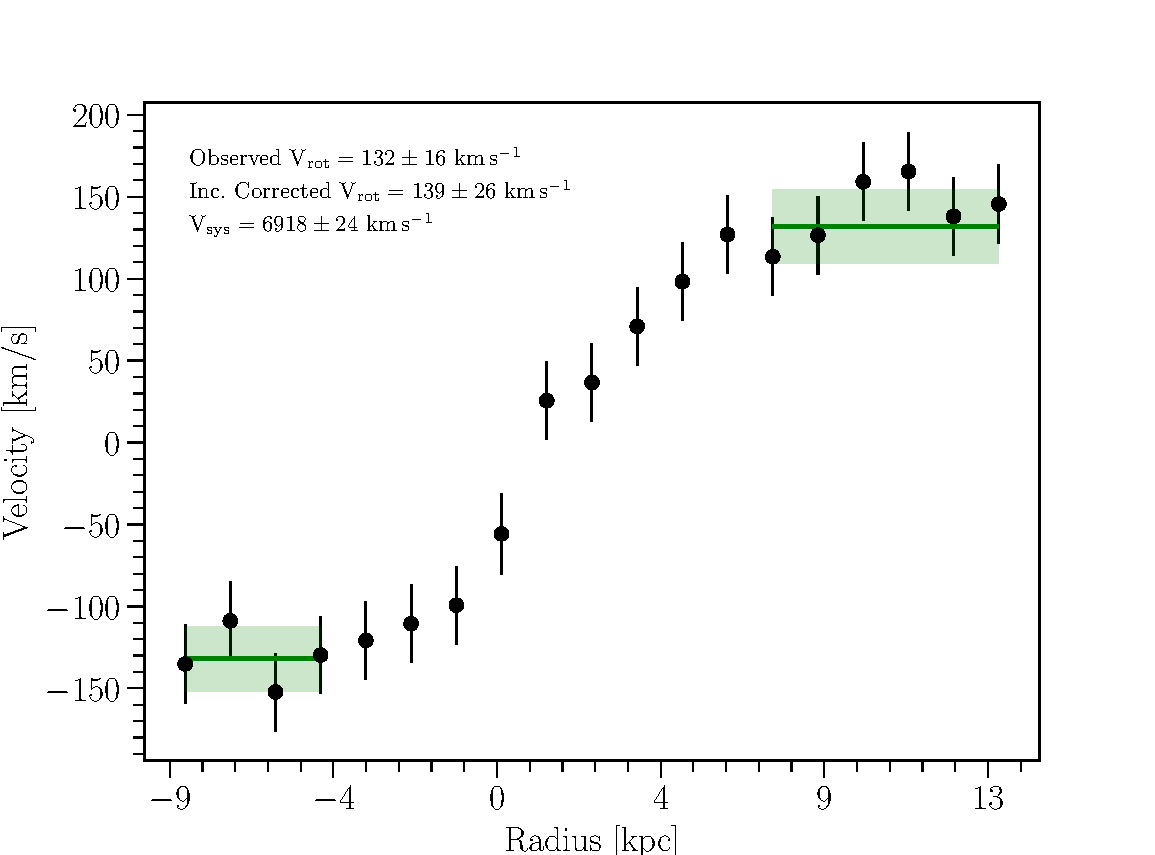
\includegraphics[width=.54\linewidth]{Chap4/figures/CGCG039-137_2_rotation_curve_xphys_helio_vobs_vrotObs_new4.pdf}}{\label{rotationcurve_CGCG039-137}}
  \subfigure[]{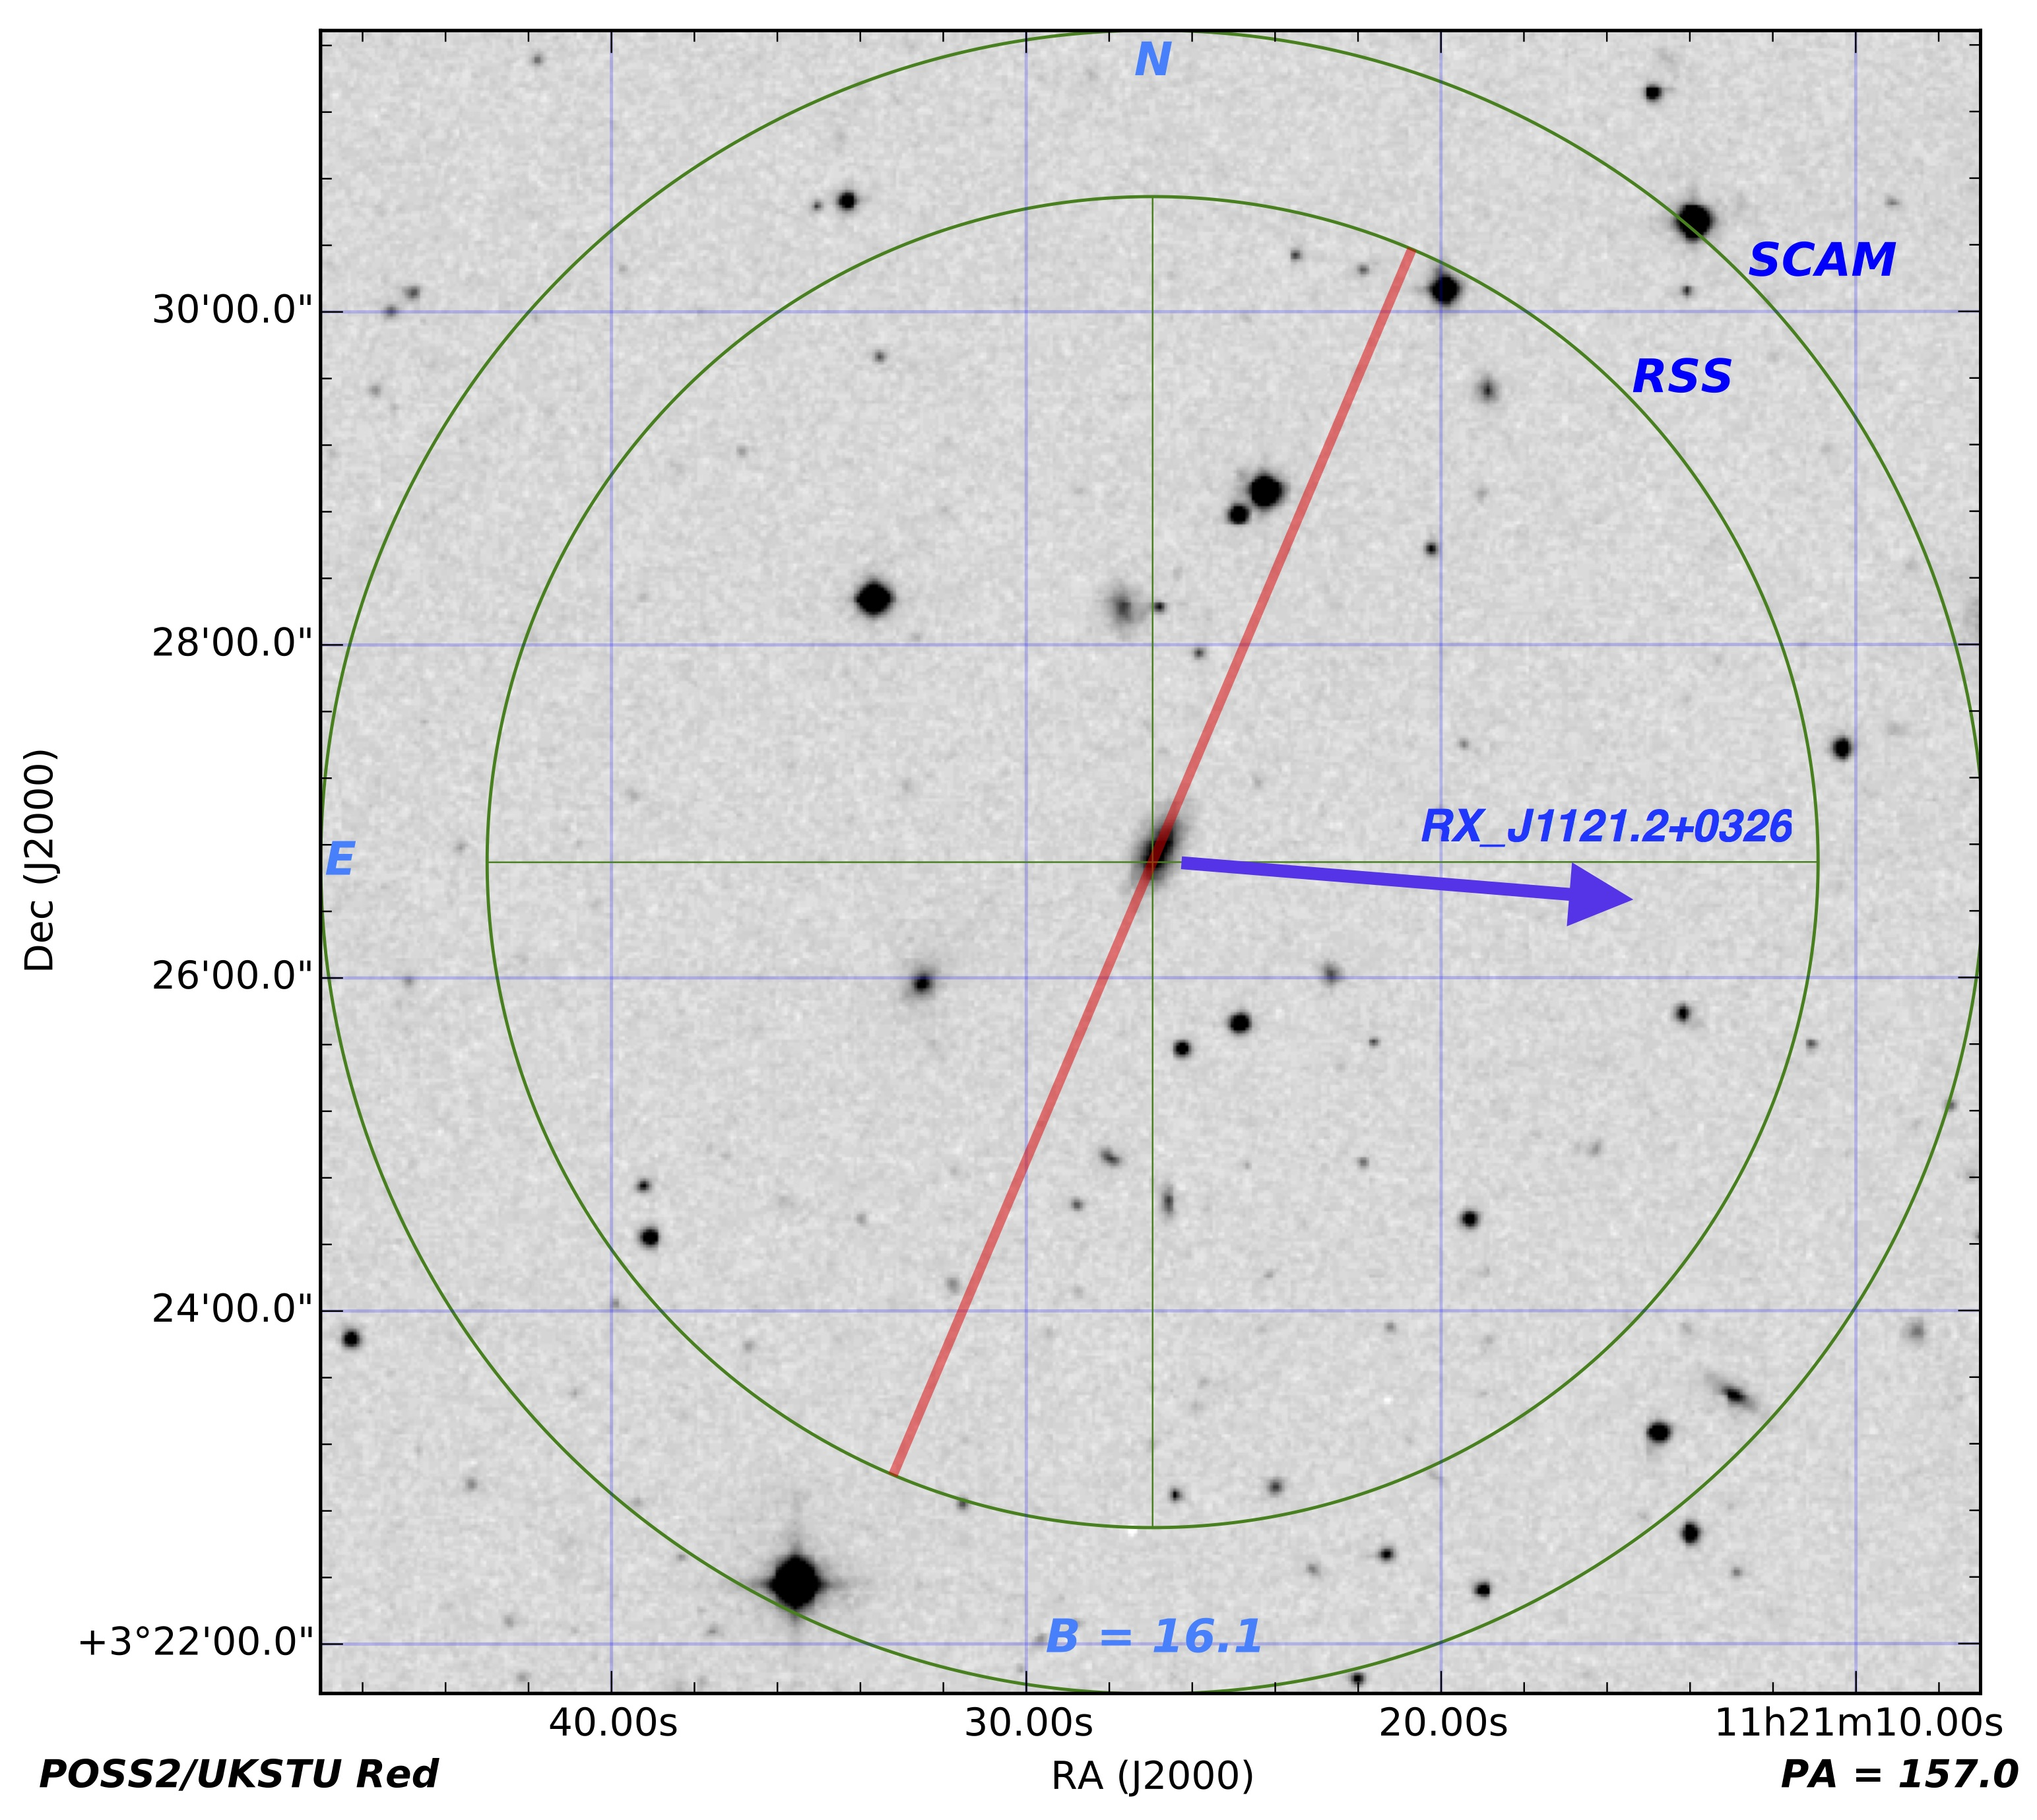
\includegraphics[width=0.45\linewidth]{Chap4/figures/CGCG039-137_Finding_chart.jpg}\label{finderchart_CGCG039-137}}
  \caption{\small{a) Rotation curve of CGCG039-137. The solid green line indicates the weighted mean velocity over the corresponding x-axis region, and the shaded green indicates the 1$\sigma$ error in the mean. b) SALT finder chart for CGCG039-137 showing the position of the slit in red.}}
\vspace{0pt}
\end{figure}


\subsection{ESO343-G014}
ESO343-G014 is an edge-on spiral galaxy with a measured systemic velocity $v_{\rm sys} = 9139 \pm$ 32 \kms. It has a smaller neighboring galaxy, 2MASXJ21372816-3824412, located north of it's major axis at a projected distance of 216 kpc and velocity of 9129 \kms. The nearest sightline is towards RBS1768 at $\rho = 466$ kpc and $74^{\circ}$ azimuth angle on the approaching side. We detect 3 blended Ly$\rm \alpha$ absorption components toward RBS1768 at $v_{\rm Ly\alpha} = 9308, 9360, 9434$ \kms~($\Delta v = 169, 221, 295$ \kms). This system is highly blended with galactic S\,{\sc ii}, and therefore their widths are not reliable. All of these are anti-aligned with the rotation of ESO343-G014 relative to the models (cylindrical = [-203, 10], NFW = [-122, 31] \kms). Unfortunately the presence of 2MASXJ21372816-3824412 makes it difficult to attribute this gas solely to ESO343-G014. Additionally, this gas could be attributed to either the approaching or receding side of the disk due to the large impact parameter and high azimuth angle of the sightline.

\begin{figure}[ht]
\centering
  \subfigure[]{\includegraphics[width=.54\linewidth]{Chap4/figures/RFGC3781_2_rotation_curve_xphys_helio_vobs_vrotObs_new4.pdf}}{\label{rotationcurve_ESO343-G014}}
  \subfigure[]{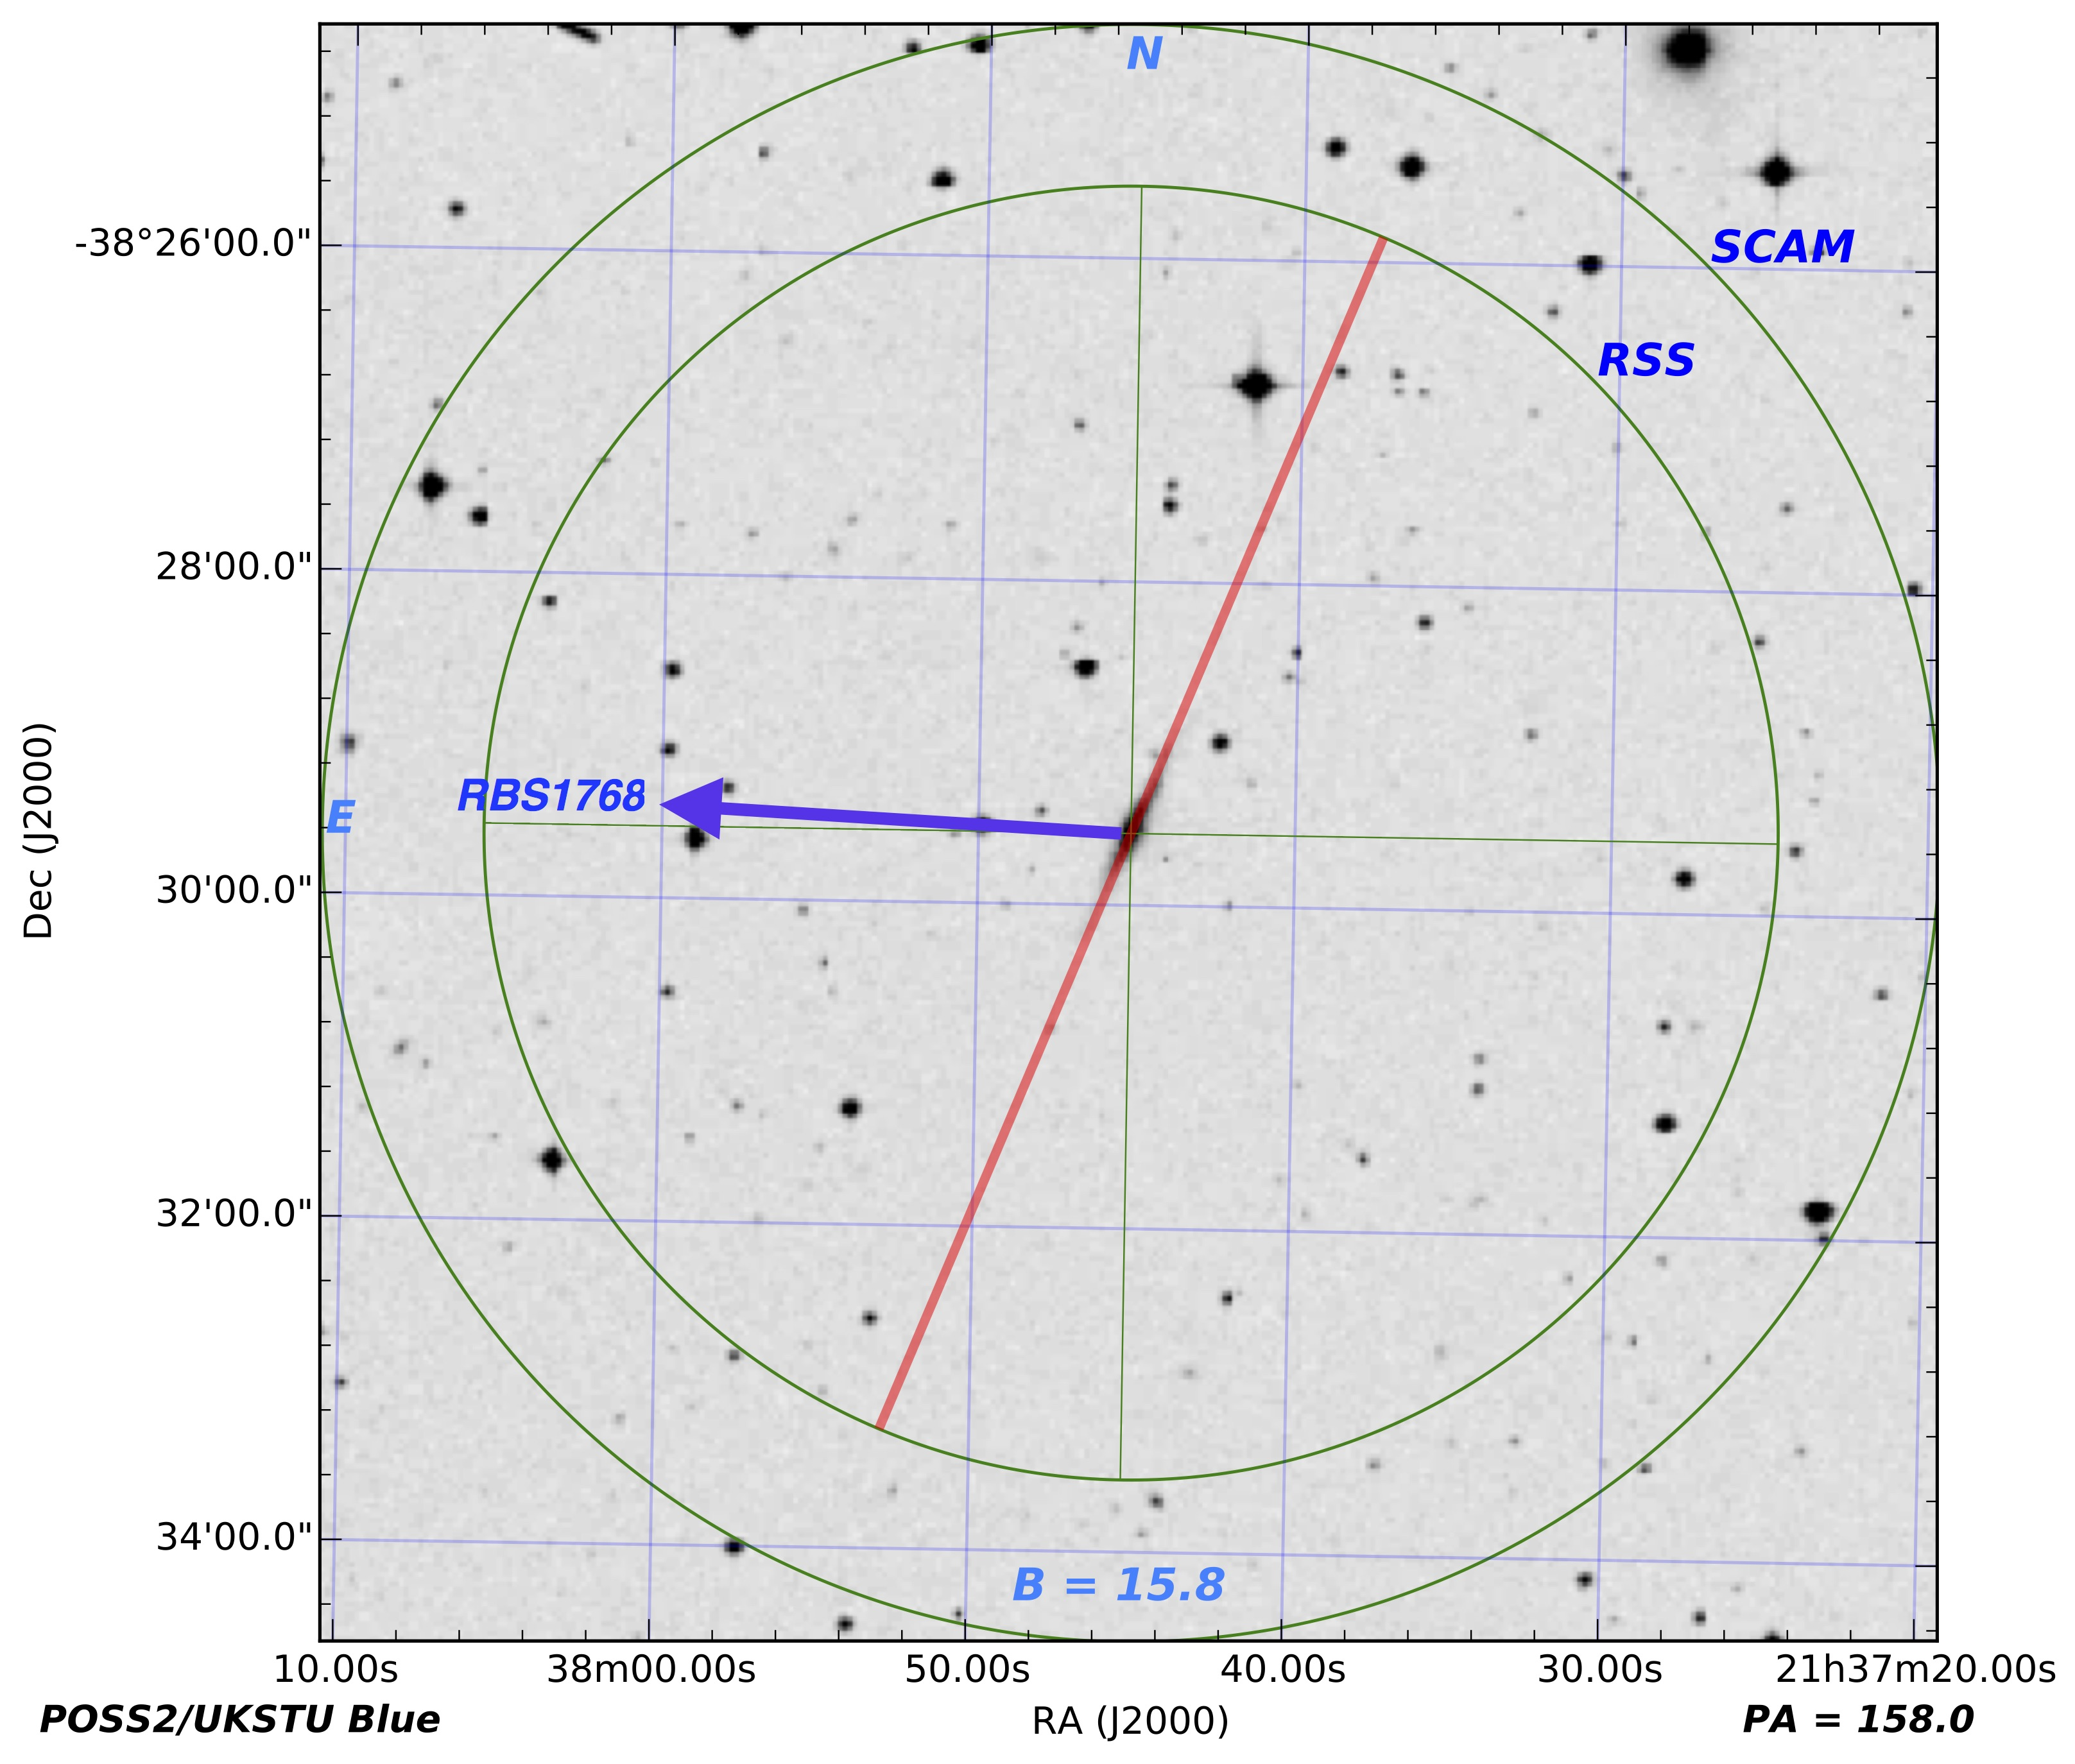
\includegraphics[width=0.45\linewidth]{Chap4/figures/RFGC3781_FindingChart.jpg}\label{finderchart_ESO343-G014}}
  \caption{\small{a) Rotation curve of ESO343-G014. The solid green line indicates the weighted mean velocity over the corresponding x-axis region, and the shaded green indicates the 1$\sigma$ error in the mean. b) SALT finder chart for ESO343-G014 showing the position of the slit in red.}}
\vspace{0pt}
\end{figure}


\subsection{IC5325}
IC5325 is a mostly face-on SAB(rs)bc type galaxy with a measured systemic velocity $v_{\rm sys} = 1512 \pm 8$ \kms. It's inclination is just high enough ($i = 25^{\circ}$) to obtain a reasonable rotation curve. The closest neighboring galaxy is ESO347-G020 to the southeast at 306 kpc and $v_{sys} = 1745$ \kms. Three other much smaller galaxies are also located $\sim 450$ kpc to the southwest. The background QSO RBS2000 is located northeast at $\rho = 314$ kpc and  $64^{\circ}$ azimuth angle on the approaching side of IC5325. We detect Ly$\alpha$ at $v_{\rm Ly\alpha} = 1598$ \kms~($\Delta v = 86$ \kms) towards RBS2000. While this velocity is anti-aligned with the rotation the disk gas relative to our model predictions (cylindrical = [-41, -20], NFW = [-29, 1] \kms), the low inclination angle of IC5325 leads to a highly uncertain position angle. Without additional observations, we cannot say for certain if the location of RBS2000 actually lies on the approaching or receding side. This position angle uncertainty also means our SALT rotation curve is a lower limit on the true rotation velocity of IC5325.

\begin{figure}[ht]
\centering
  \subfigure[]{\includegraphics[width=.54\linewidth]{Chap4/figures/IC5325_2_rotation_curve_xphys_helio_vobs_vrotObs_new4.pdf}}{\label{rotationcurve_IC5325}}
  \subfigure[]{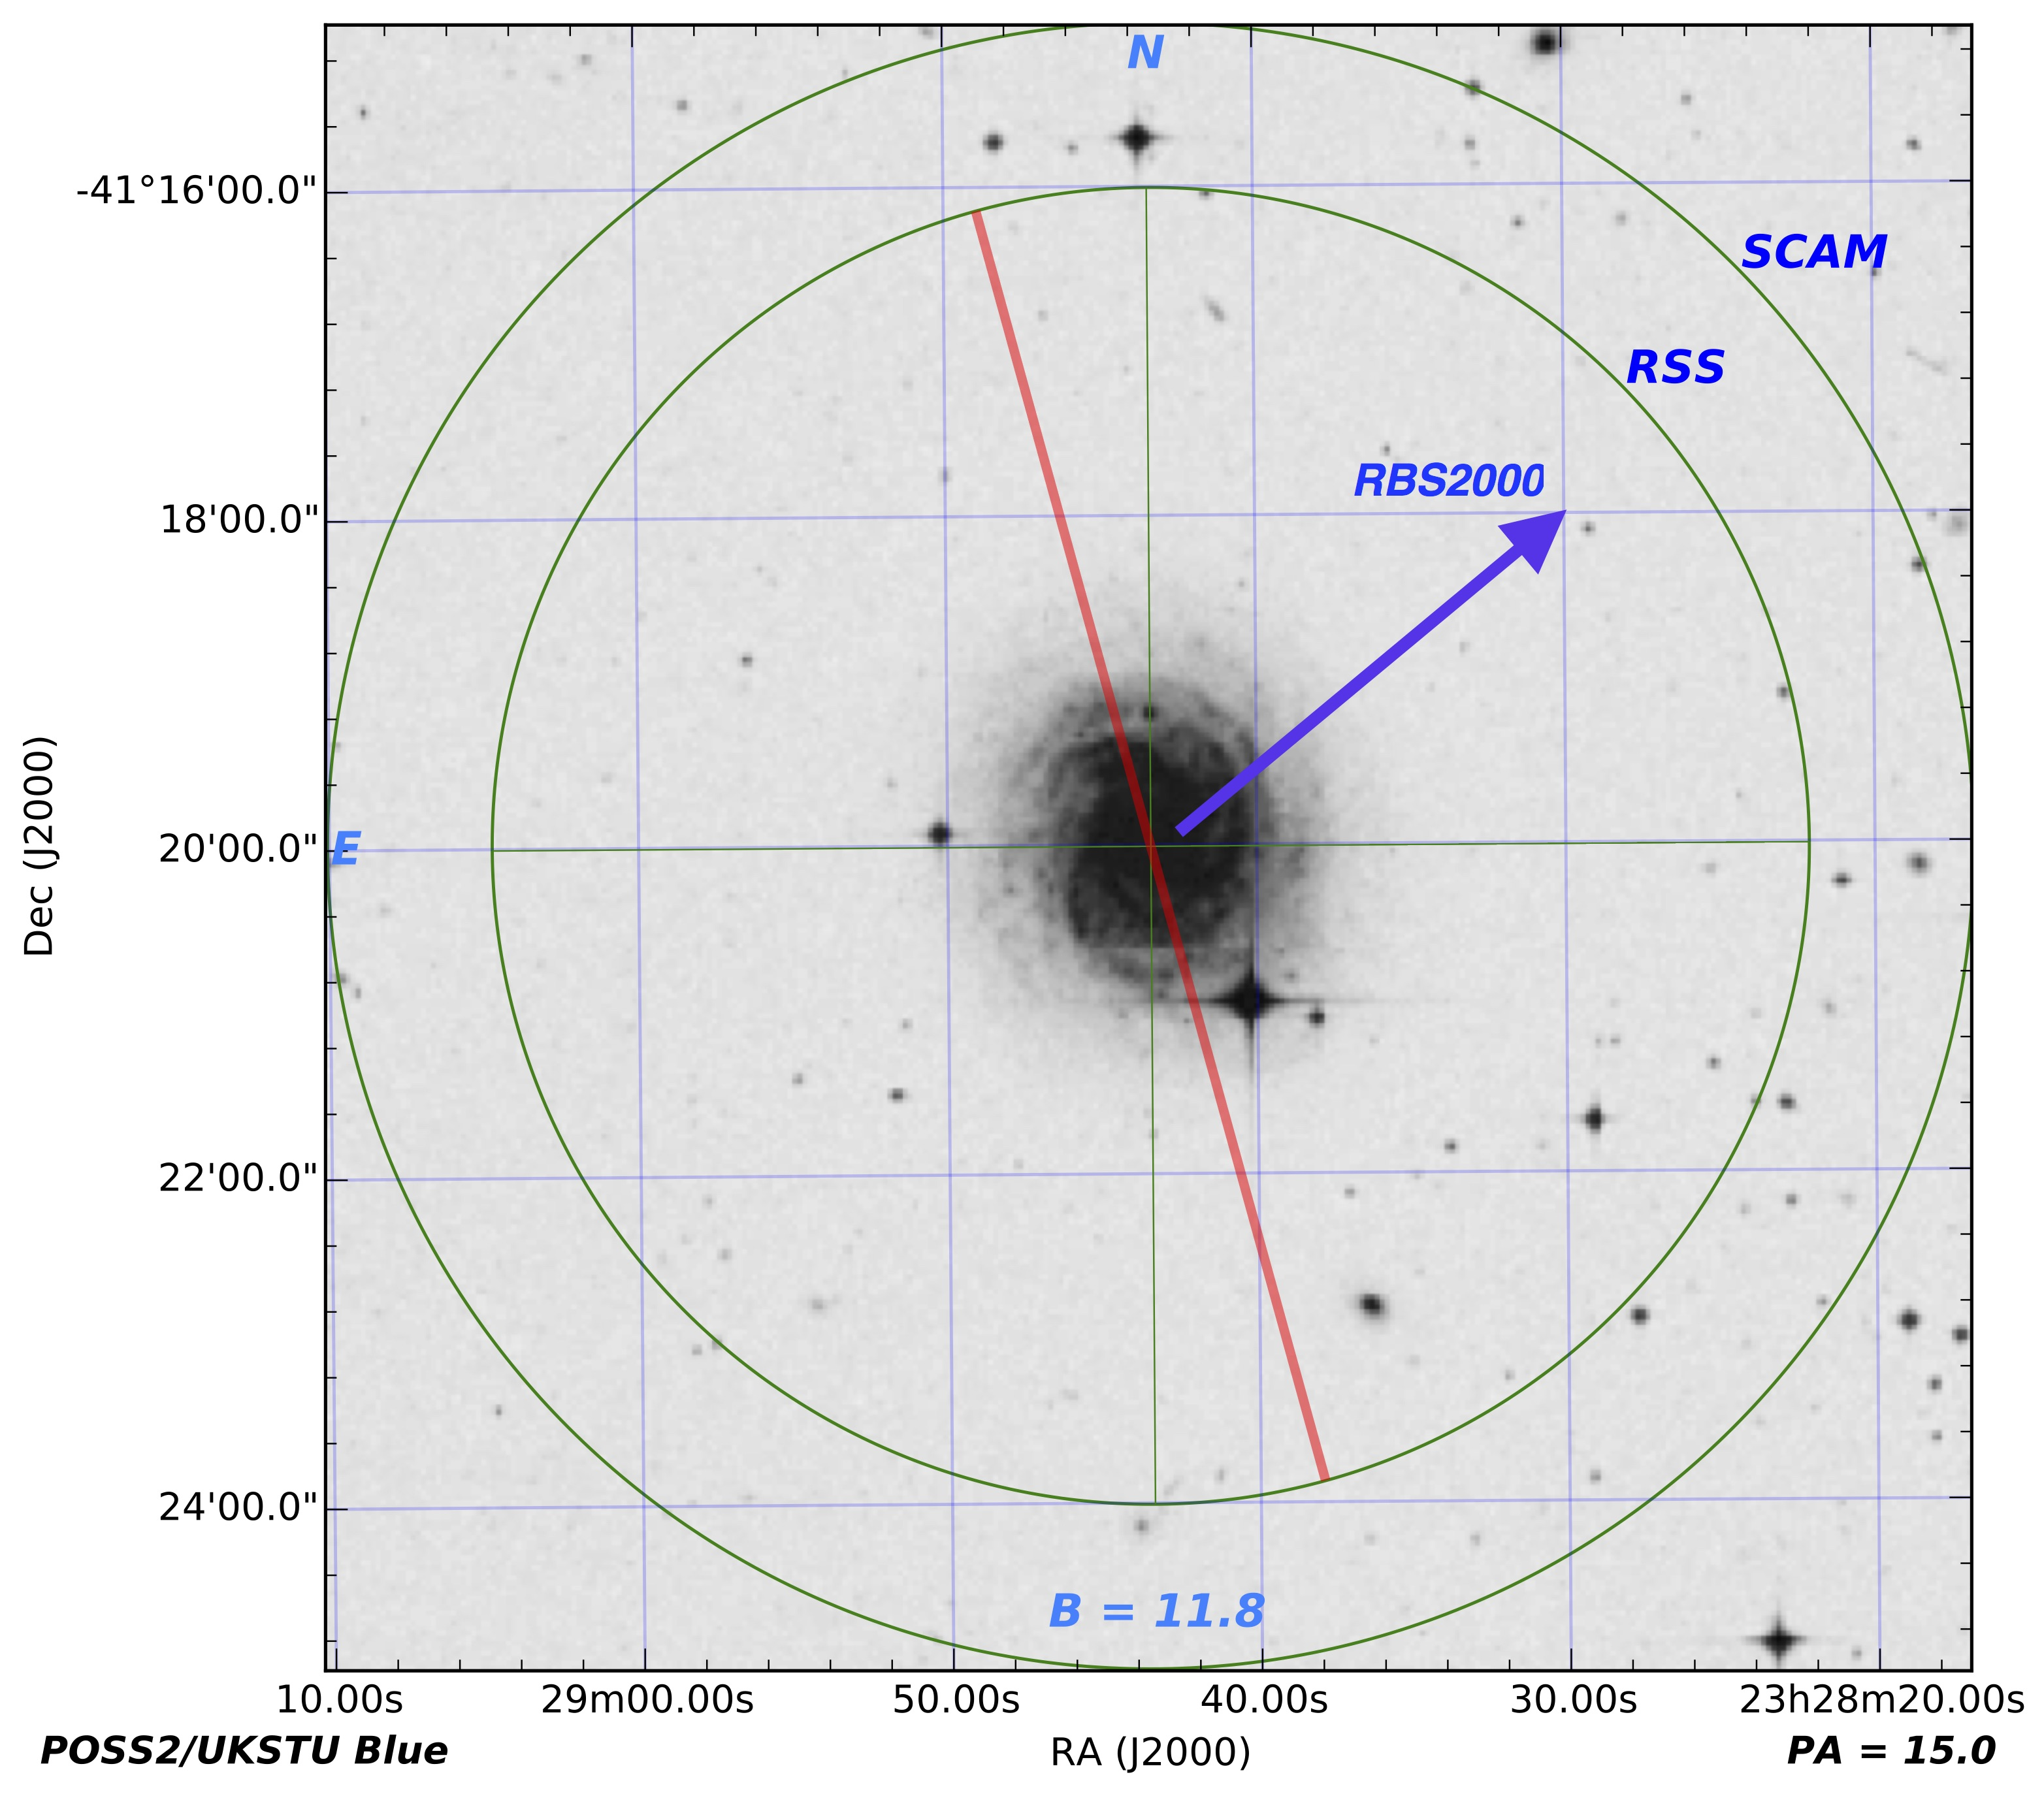
\includegraphics[width=0.45\linewidth]{Chap4/figures/IC5325_FindingChart.jpg}\label{finderchart_IC5325}}
  \caption{\small{a) Rotation curve of IC5325. The solid green line indicates the weighted mean velocity over the corresponding x-axis region, and the shaded green indicates the 1$\sigma$ error in the mean. b) SALT finder chart for IC5325 showing the position of the slit in red.}}
\vspace{0pt}
\end{figure}


%The velocity of the absorber, $\Delta v = 86$\kms, is also outside the range of projected co-rotation velocities

% Two galaxies are neighboring IC5325 to the South and East: PGC071660 at XXX kpc and NGC7552 at XXX kpc. 


\subsection{MCG-03-58-009}
MCG-03-58-009 is a massive and very isolated Sc type galaxy at a measured systemic velocity of $v_{\rm sys} = 9015 \pm 19$ \kms~and inclination angle of $i = 49^{\circ}$. The background QSO MRC2251-178 is located southeast at $\rho = 355$ kpc at an azimuth angle of $71^{\circ}$ on the receding side. We detect a weak Ly$\rm \alpha$ absorber at $v_{\rm Ly\alpha} = 9029$ \kms~($\Delta v = 14$ \kms) towards MRC2251-178. This absorber velocity falls well within the expected range for co-rotation relative to our models (cylindrical = [-26, 137], NFW = [-42, 83] \kms). Although this absorber matches the velocity expected for co-rotation, the velocity difference ($\Delta v = 14$ \kms) is also within the systemic velocity uncertainty for MCG-03-58-009. The relative weakness of this absorber (EW = $62 \pm 4$ m\AA) is somewhat unusual given it's proximity (just outside of 1 $R_{vir}$) to a massive galaxy. If this is representative of an isolated system such as MCG-03-58-009, then we should expect the halo rotational velocity to approach systemic by 1 $R_{vir}$.

\begin{figure}[ht]
\centering
  \subfigure[]{\includegraphics[width=.54\linewidth]{Chap4/figures/MCG-03-58-009_2_rotation_curve_xphys_helio_vobs_vrotObs_new4.pdf}}{\label{rotationcurve_MCG-03-58-009}}
  \subfigure[]{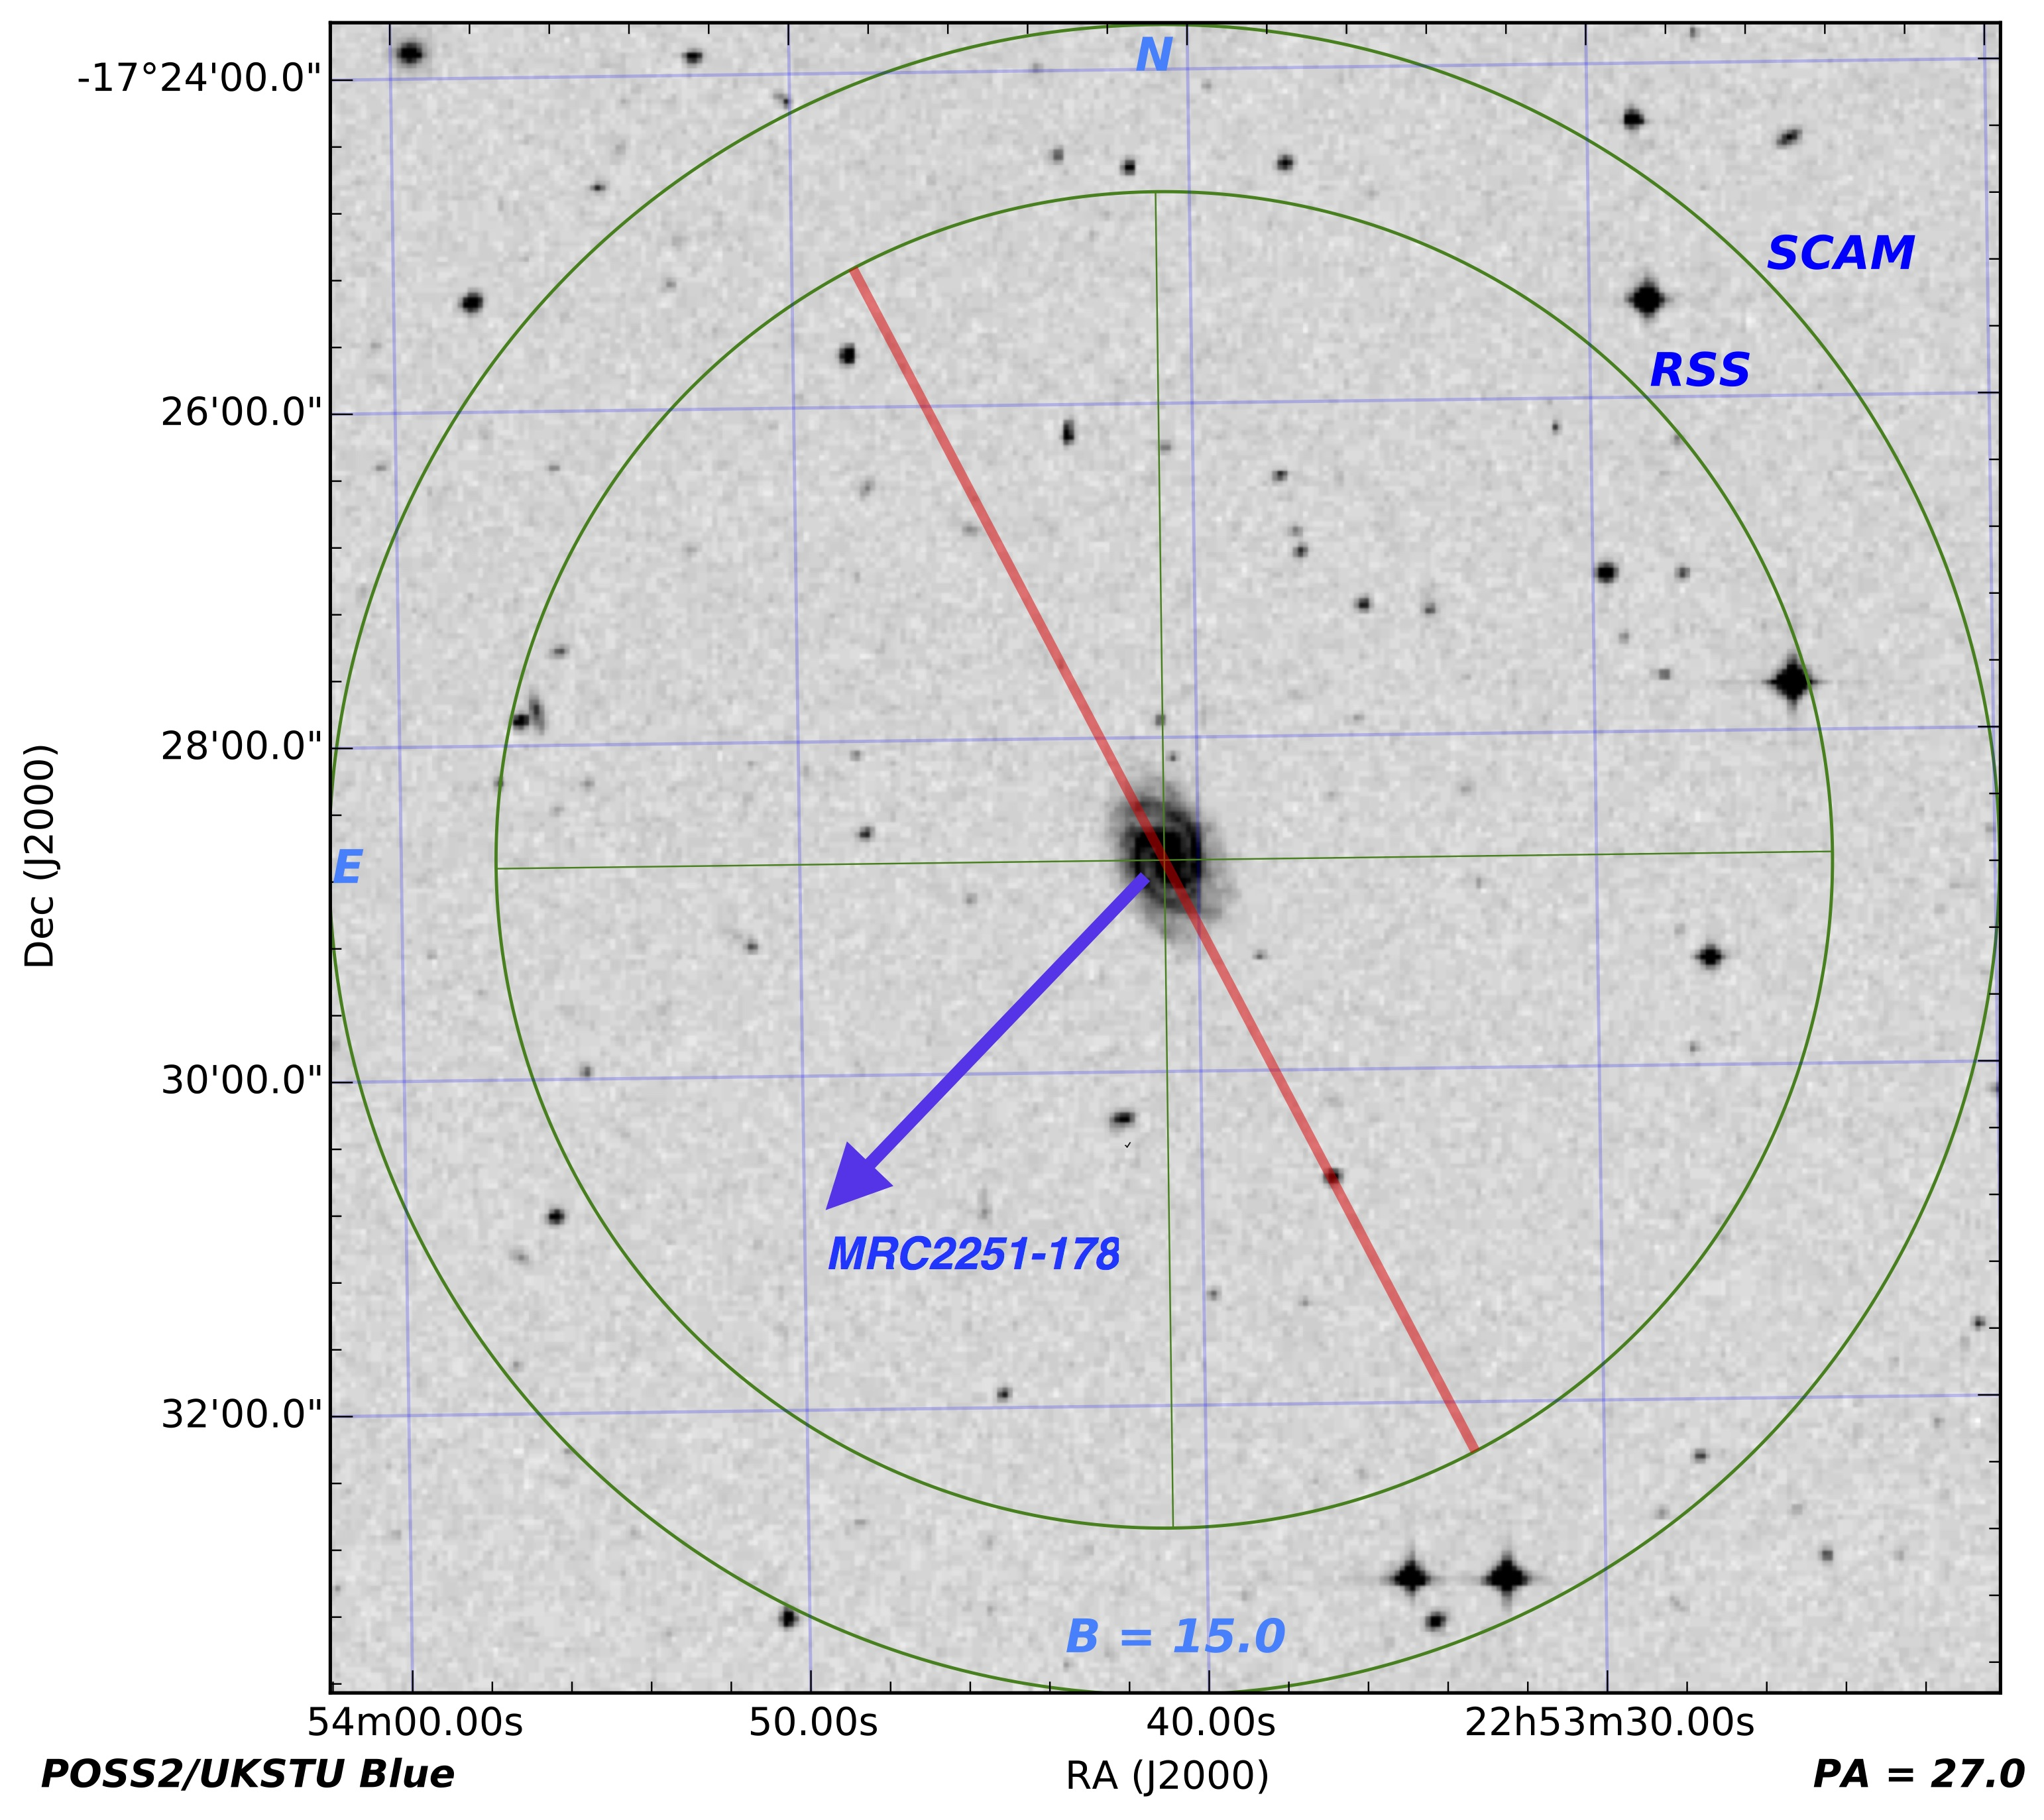
\includegraphics[width=0.45\linewidth]{Chap4/figures/MCG-03-58-009_FindingChart.jpg}\label{finderchart_MCG-03-58-009}}
  \caption{\small{a) Rotation curve of MCG-03-58-009. The solid green line indicates the weighted mean velocity over the corresponding x-axis region, and the shaded green indicates the 1$\sigma$ error in the mean. b) SALT finder chart for MCG-03-58-009 showing the position of the slit in red.}}
\vspace{0pt}
\end{figure}



\subsection{NGC1566}
NGC1566 is a SAB(rs)bc type galaxy with measured systemic velocity of $v_{\rm sys} = 1502 \pm 15$ \kms~and inclination angle of $i = 46^{\circ}$. There are several other large galaxies at $\rho \gtrsim 200$ kpc from NGC1566 (e.g., NGC1549, NGC1596, and NGC1581). The closest QSO sightline is toward HE0429-5343, northeast of NGC1566 at $\rho = 256$ kpc and $60^{\circ}$ azimuth angle. We detect Ly$\rm \alpha$ absorption toward HE0429-5343 at $v_{\rm Ly\alpha} = 1167, 1358$ \kms~($\Delta v = -335, -144$ \kms). Both of these absorbers have the correct velocity \emph{sign}, but we would expect a smaller velocity for co-rotation based on our model results (cylindrical = [-53, -2], NFW = [-22, 17] \kms). Unfortunately NGC1617 is slightly closer to this sightline than NGC1566, at $\rho = 233$ kpc and $v_{\rm sys} = 1063$ \kms, so it is not possible to confidently attribute these absorbers to NGC1566.

A more distant QSO sightline toward 1H0419-577 is located to the south at $\rho = 303$ kpc and just east of the receding side of the major axis at an azimuth angle of $10^{\circ}$. We detect Ly$\rm \alpha$ at $v_{\rm Ly\alpha} = 1123, 1188, 1264$ \kms~($\Delta v = -379, -314, -238$ \kms), all of which are the wrong sign for co-rotation relative to our models (cylindrical = [48, 76], NFW = [-2, 31] \kms). This sightline is \emph{also} actually closer to a small group of galaxies including NGC1549, NGC1546 and NGC1536, all with systemic velocities near $\sim 1200$ \kms. Additionally, this absorber system contains C\,{\sc iii}, C\,{\sc iv}, Si\,{\sc ii}, Si\,{\sc iii}, Si\,{\sc iv} lines. These lines likely are associated with this group rather than with NGC1566. 

\begin{figure}[ht]
\centering
  \subfigure[]{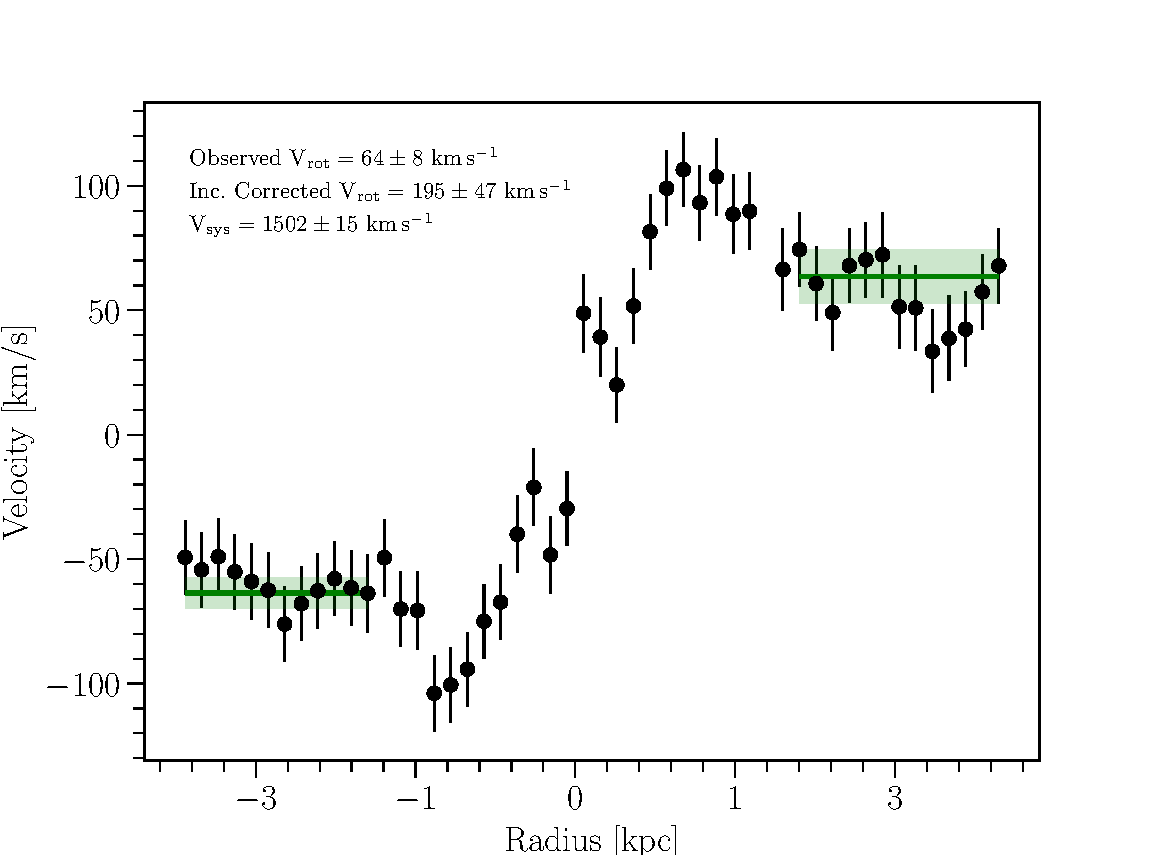
\includegraphics[width=.54\linewidth]{Chap4/figures/NGC1566_2_rotation_curve_xphys_helio_vobs_vrotObs_new4.pdf}}{\label{rotationcurve_NGC1566}}
  \subfigure[]{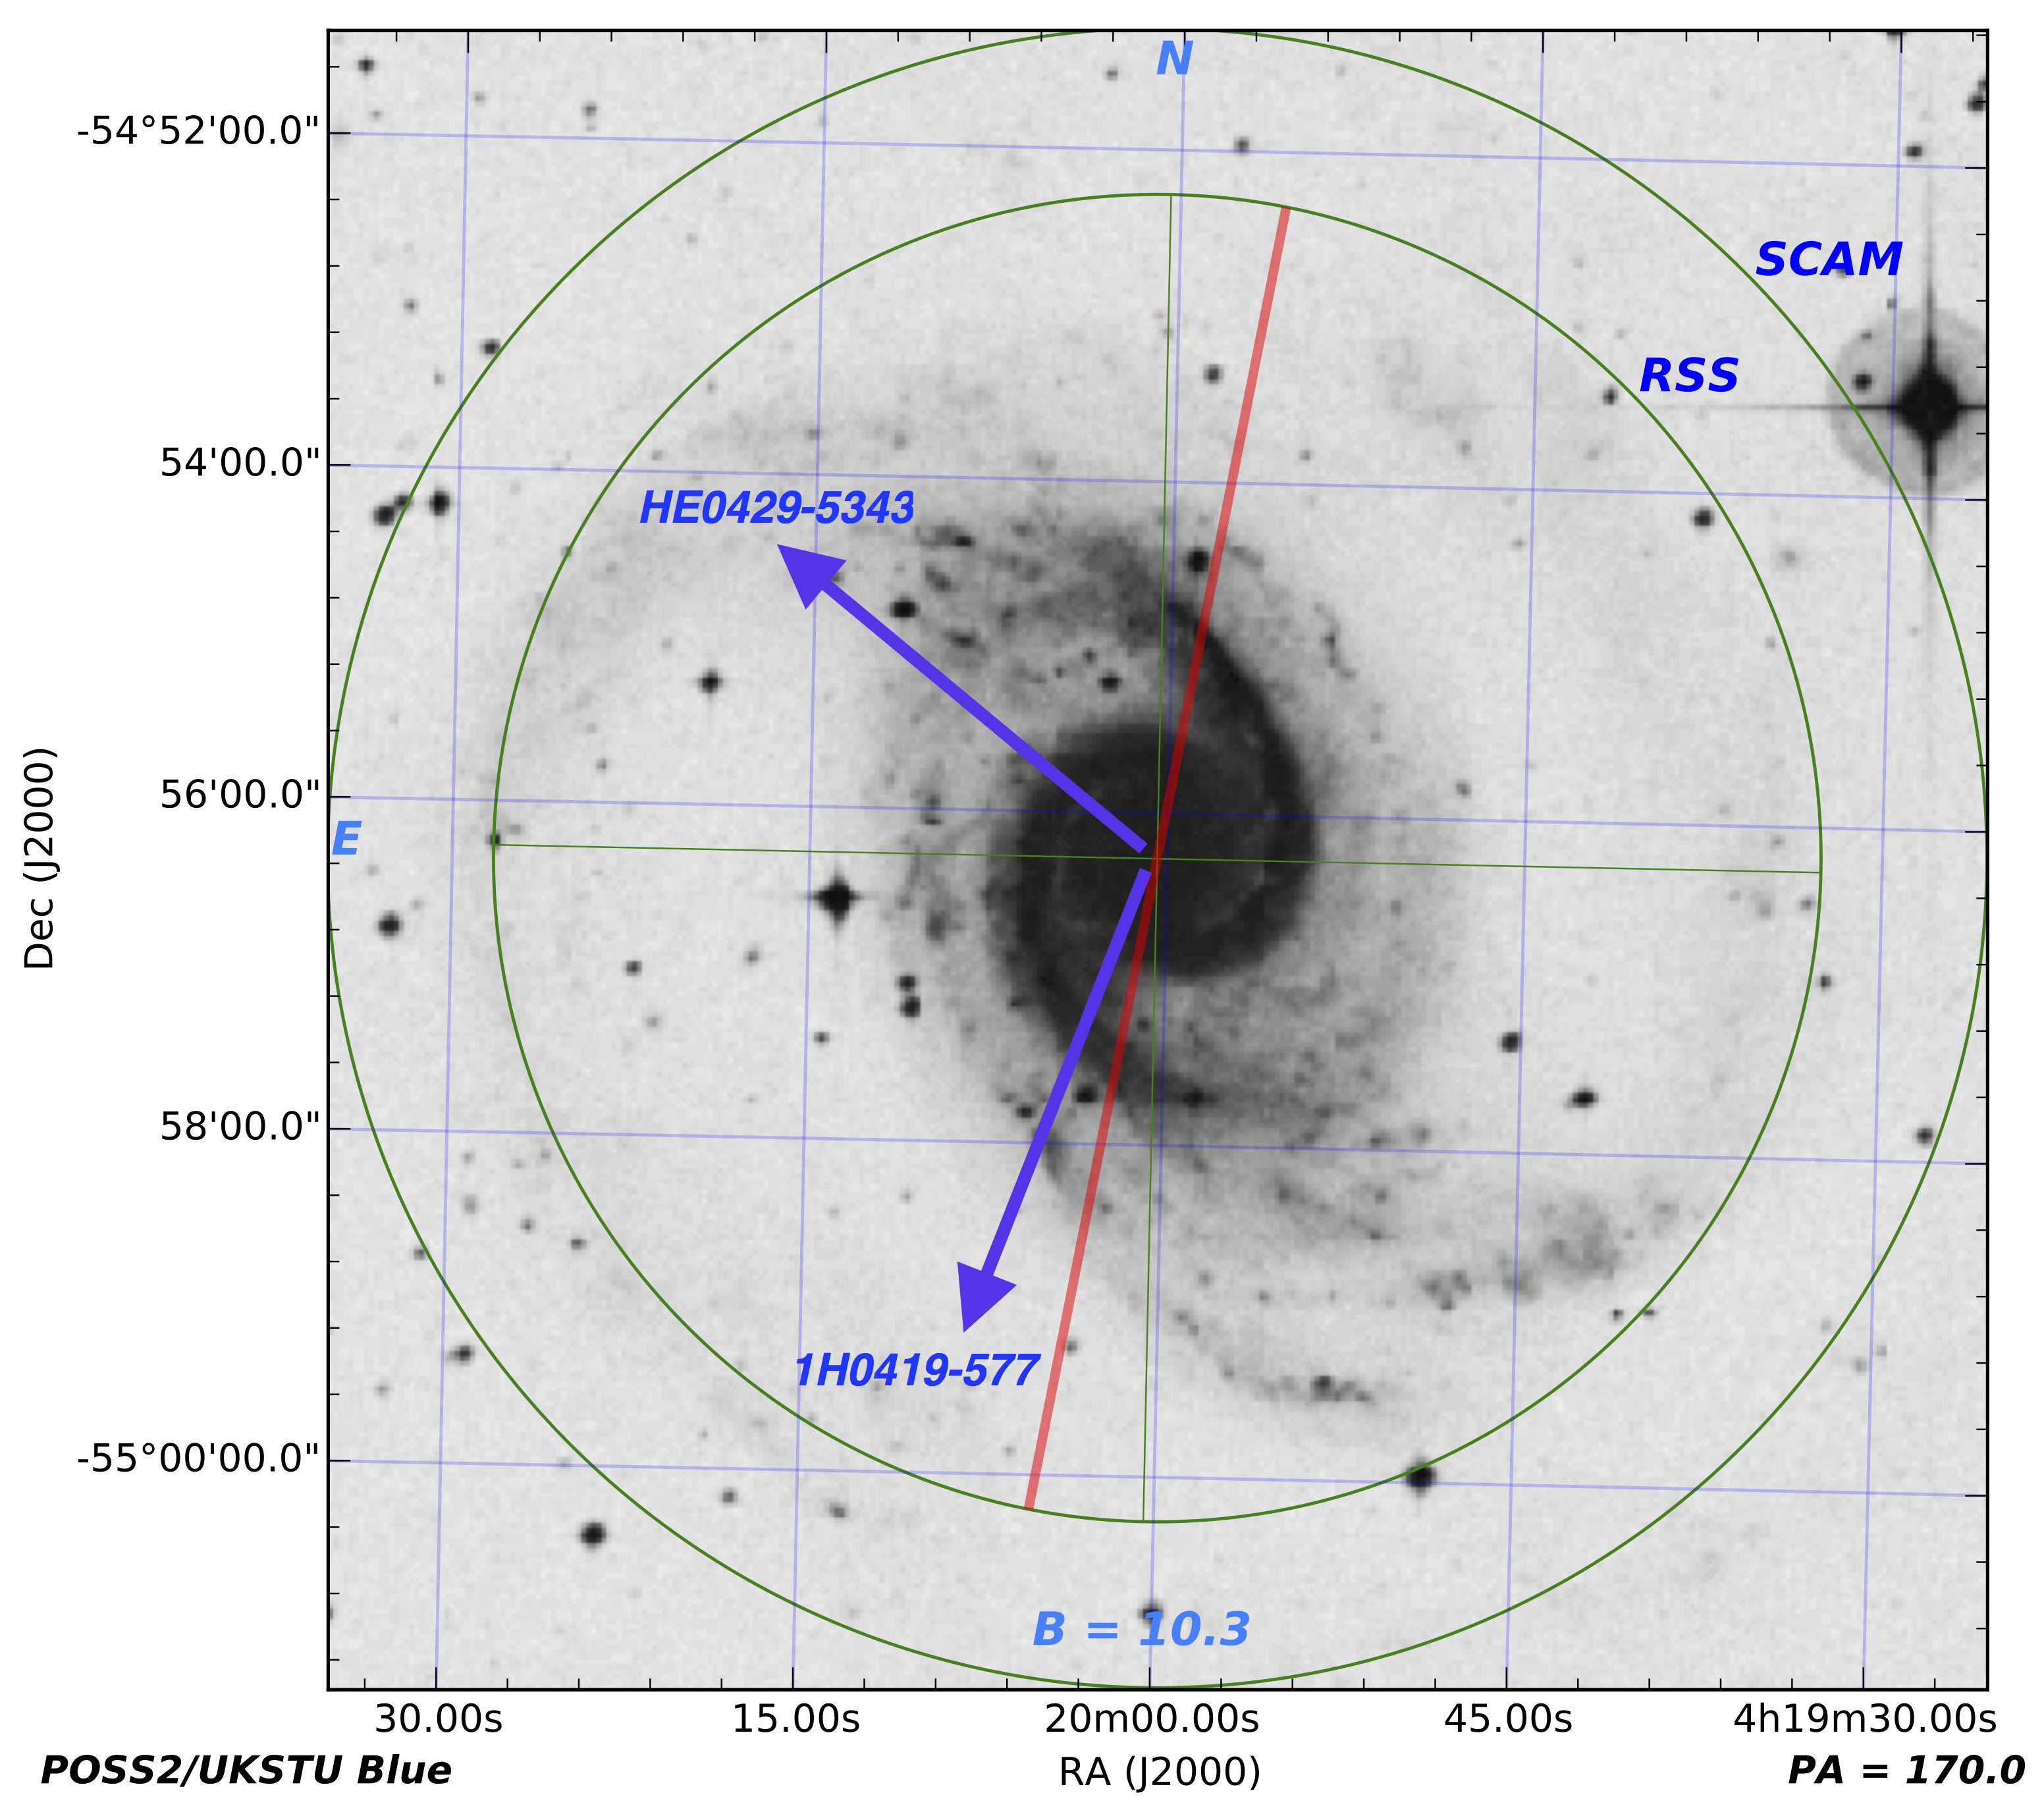
\includegraphics[width=0.45\linewidth]{Chap4/figures/NGC1566_FindingChart.jpg}\label{finderchart_NGC1566}}
  \caption{\small{a) Rotation curve of NGC1566. The solid green line indicates the weighted mean velocity over the corresponding x-axis region, and the shaded green indicates the 1$\sigma$ error in the mean. b) SALT finder chart for NGC1566 showing the position of the slit in red.}}
\vspace{0pt}
\end{figure}

%(approximately $\Delta v \sim \pm40$ \kms~projected).

%NGC1566 is well sampled (5 nearby QSO sightlines), but unfortunately also part of a complex environment of neighboring galaxies. 

%We detect Ly$\alpha$ in all 5 of these sightlines. The farthest three, HE0439-5254, RBS567, and HE0435-5304, are clustered close together toward the northeast of NGC1566 at 459, 423, and 396 kpc and $\sim 60^{\circ}$ azimuth angle. HE0439-5254 and RBS567 are both located beyond our 2 x 3 $R_{vir}$ model limits and therefore are only included here for the sake of completeness. The slightly closer HE0435-5304 sneaks under the limit.

%HE0429-5343 is in the same direction and azimuth angle but closer at $\rho = 256$ kpc, and shows Ly$\alpha$ absorption at 1167 and 1358 \kms. These absorbers both have the correct velocity \emph{sign}, but we would expect a smaller velocity for co-rotation (approximately $\Delta v \sim \pm40$ \kms~projected). This difference could be explained by invoking either a warped extended disk, or perhaps inflowing gas.



\subsection{NGC3513}
NGC3513 a mostly face-on SB(rs)c galaxy with measured systemic velocity $v_{\rm sys} = 1204 \pm 12$ \kms. It has a companion galaxy in NGC3511 at $\rho = 44$ kpc and $v_{\rm sys} = 1109$ \kms~(NGC3513 diameter $D = 22.1$ kpc, NGC3511 diameter $D = 28.1$ kpc). The background QSO H1101-232 is located directly south of the pair at $\rho = 60$ kpc and azimuth angle of $67^{\circ}$ on the receding side. We detect Ly$\rm \alpha$ at $v_{\rm Ly\alpha} = 1182$ \kms~($\Delta v = -22$ \kms) toward H1101-232. NGC3513 appears to be rotating slowly, with a maximal inclination-corrected rotation velocity of $v_{\rm rot} / \sin(\emph{i}) = 22 \pm 24$ \kms. The $\Delta v = -22$ \kms~for this absorber is opposite in sign for co-rotation on the sky and just outside our predicted model velocity range (cylindrical = [-19, 27], NFW = [-19, 28] \kms). Given that NGC3511 is so close, this absorber's velocity is probably subject to a complex velocity field influenced by both NGC3511 and NGC3513. For this reason we have marked this galaxy as ``uncertain" in all map plots and have not included it in our statistical results. This absorber system also contains C\,{\sc iv}, N\,{\sc v}, Si\,{\sc ii}, Si\,{\sc iii}, and Si\,{\sc iv} lines.

\begin{figure}[hb]
\centering
  \subfigure[]{\includegraphics[width=.54\linewidth]{Chap4/figures/NGC3513_2_rotation_curve_xphys_helio_vobs_vrotObs_new4.pdf}}{\label{rotationcurve_NGC3513}}
  \subfigure[]{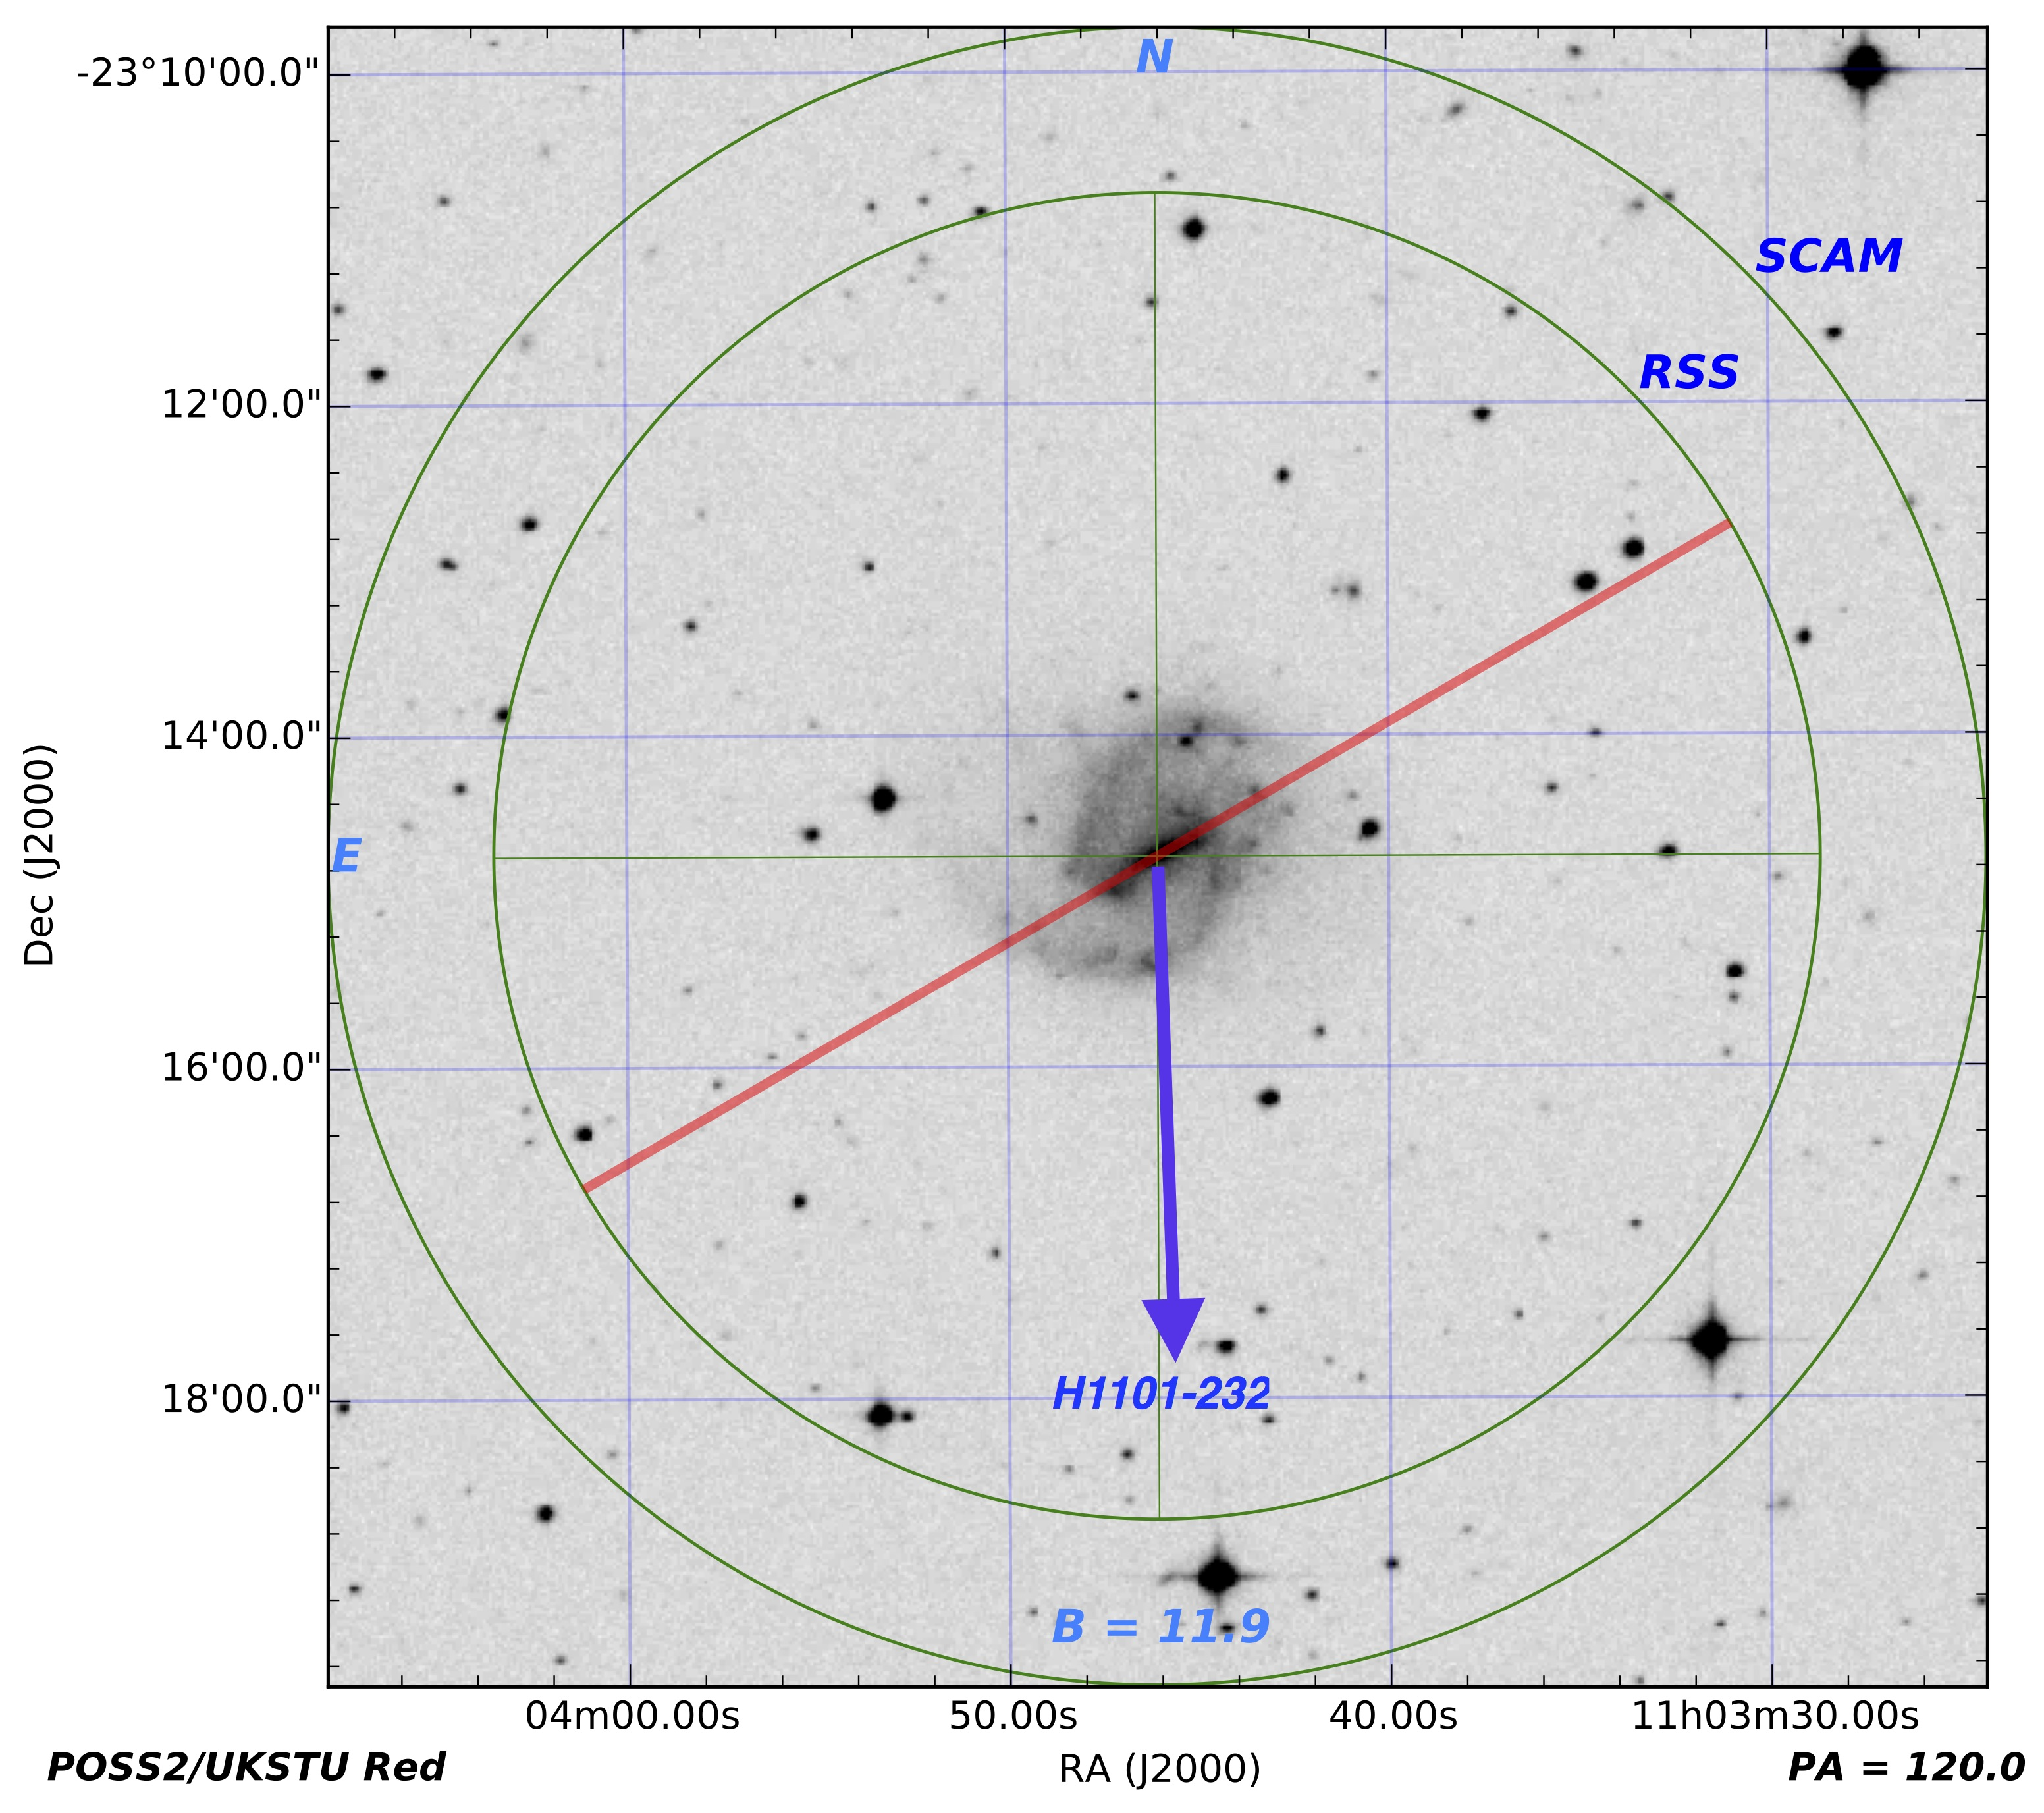
\includegraphics[width=0.45\linewidth]{Chap4/figures/NGC3513_Finding_chart.jpg}\label{finderchart_NGC3513}}
  \caption{\small{a) Rotation curve of NGC3513. The solid green line indicates the weighted mean velocity over the corresponding x-axis region, and the shaded green indicates the 1$\sigma$ error in the mean. b) SALT finder chart for NGC3513 showing the position of the slit in red.}}
\vspace{0pt}
\end{figure}



\subsection{NGC3633}
NGC3633 is an isolated, edge-on SAa type galaxy with a measured systemic velocity $v_{\rm sys} = 2587 \pm 7$ \kms. Several locations along the disk of NGC3633 show two velocities for emission. We have combined these into a single velocity measurement via a weighted average. 

The background QSO RX\_J1121.2+0326 is located southeast at $\rho = 184$ kpc and $58^{\circ}$ azimuth on the approaching side of NGC3633. We detect Ly$\rm \alpha$ at $v_{\rm Ly\alpha} = 2605$ \kms~($\Delta v = 18$ \kms) toward RX\_J1121.2+0326. While close to $v_{\rm sys}$, this absorber velocity is just outside our predicted model velocities (cylindrical = [-153, -14], NFW = [-77, 10] \kms). However, this absorber is also very weak and broad, making the velocity center uncertain by at least $\sim 10$ \kms. Taking this along with the uncertainty in $V_{\rm sys}$, this absorber could still be consistent with co-rotation.

\begin{figure}[ht]
\centering
  \subfigure[]{\includegraphics[width=.54\linewidth]{Chap4/figures/NGC3633_2_rotation_curve_xphys_helio_vobs_vrotObs_new4.pdf}}{\label{rotationcurve_NGC3633}}
  \subfigure[]{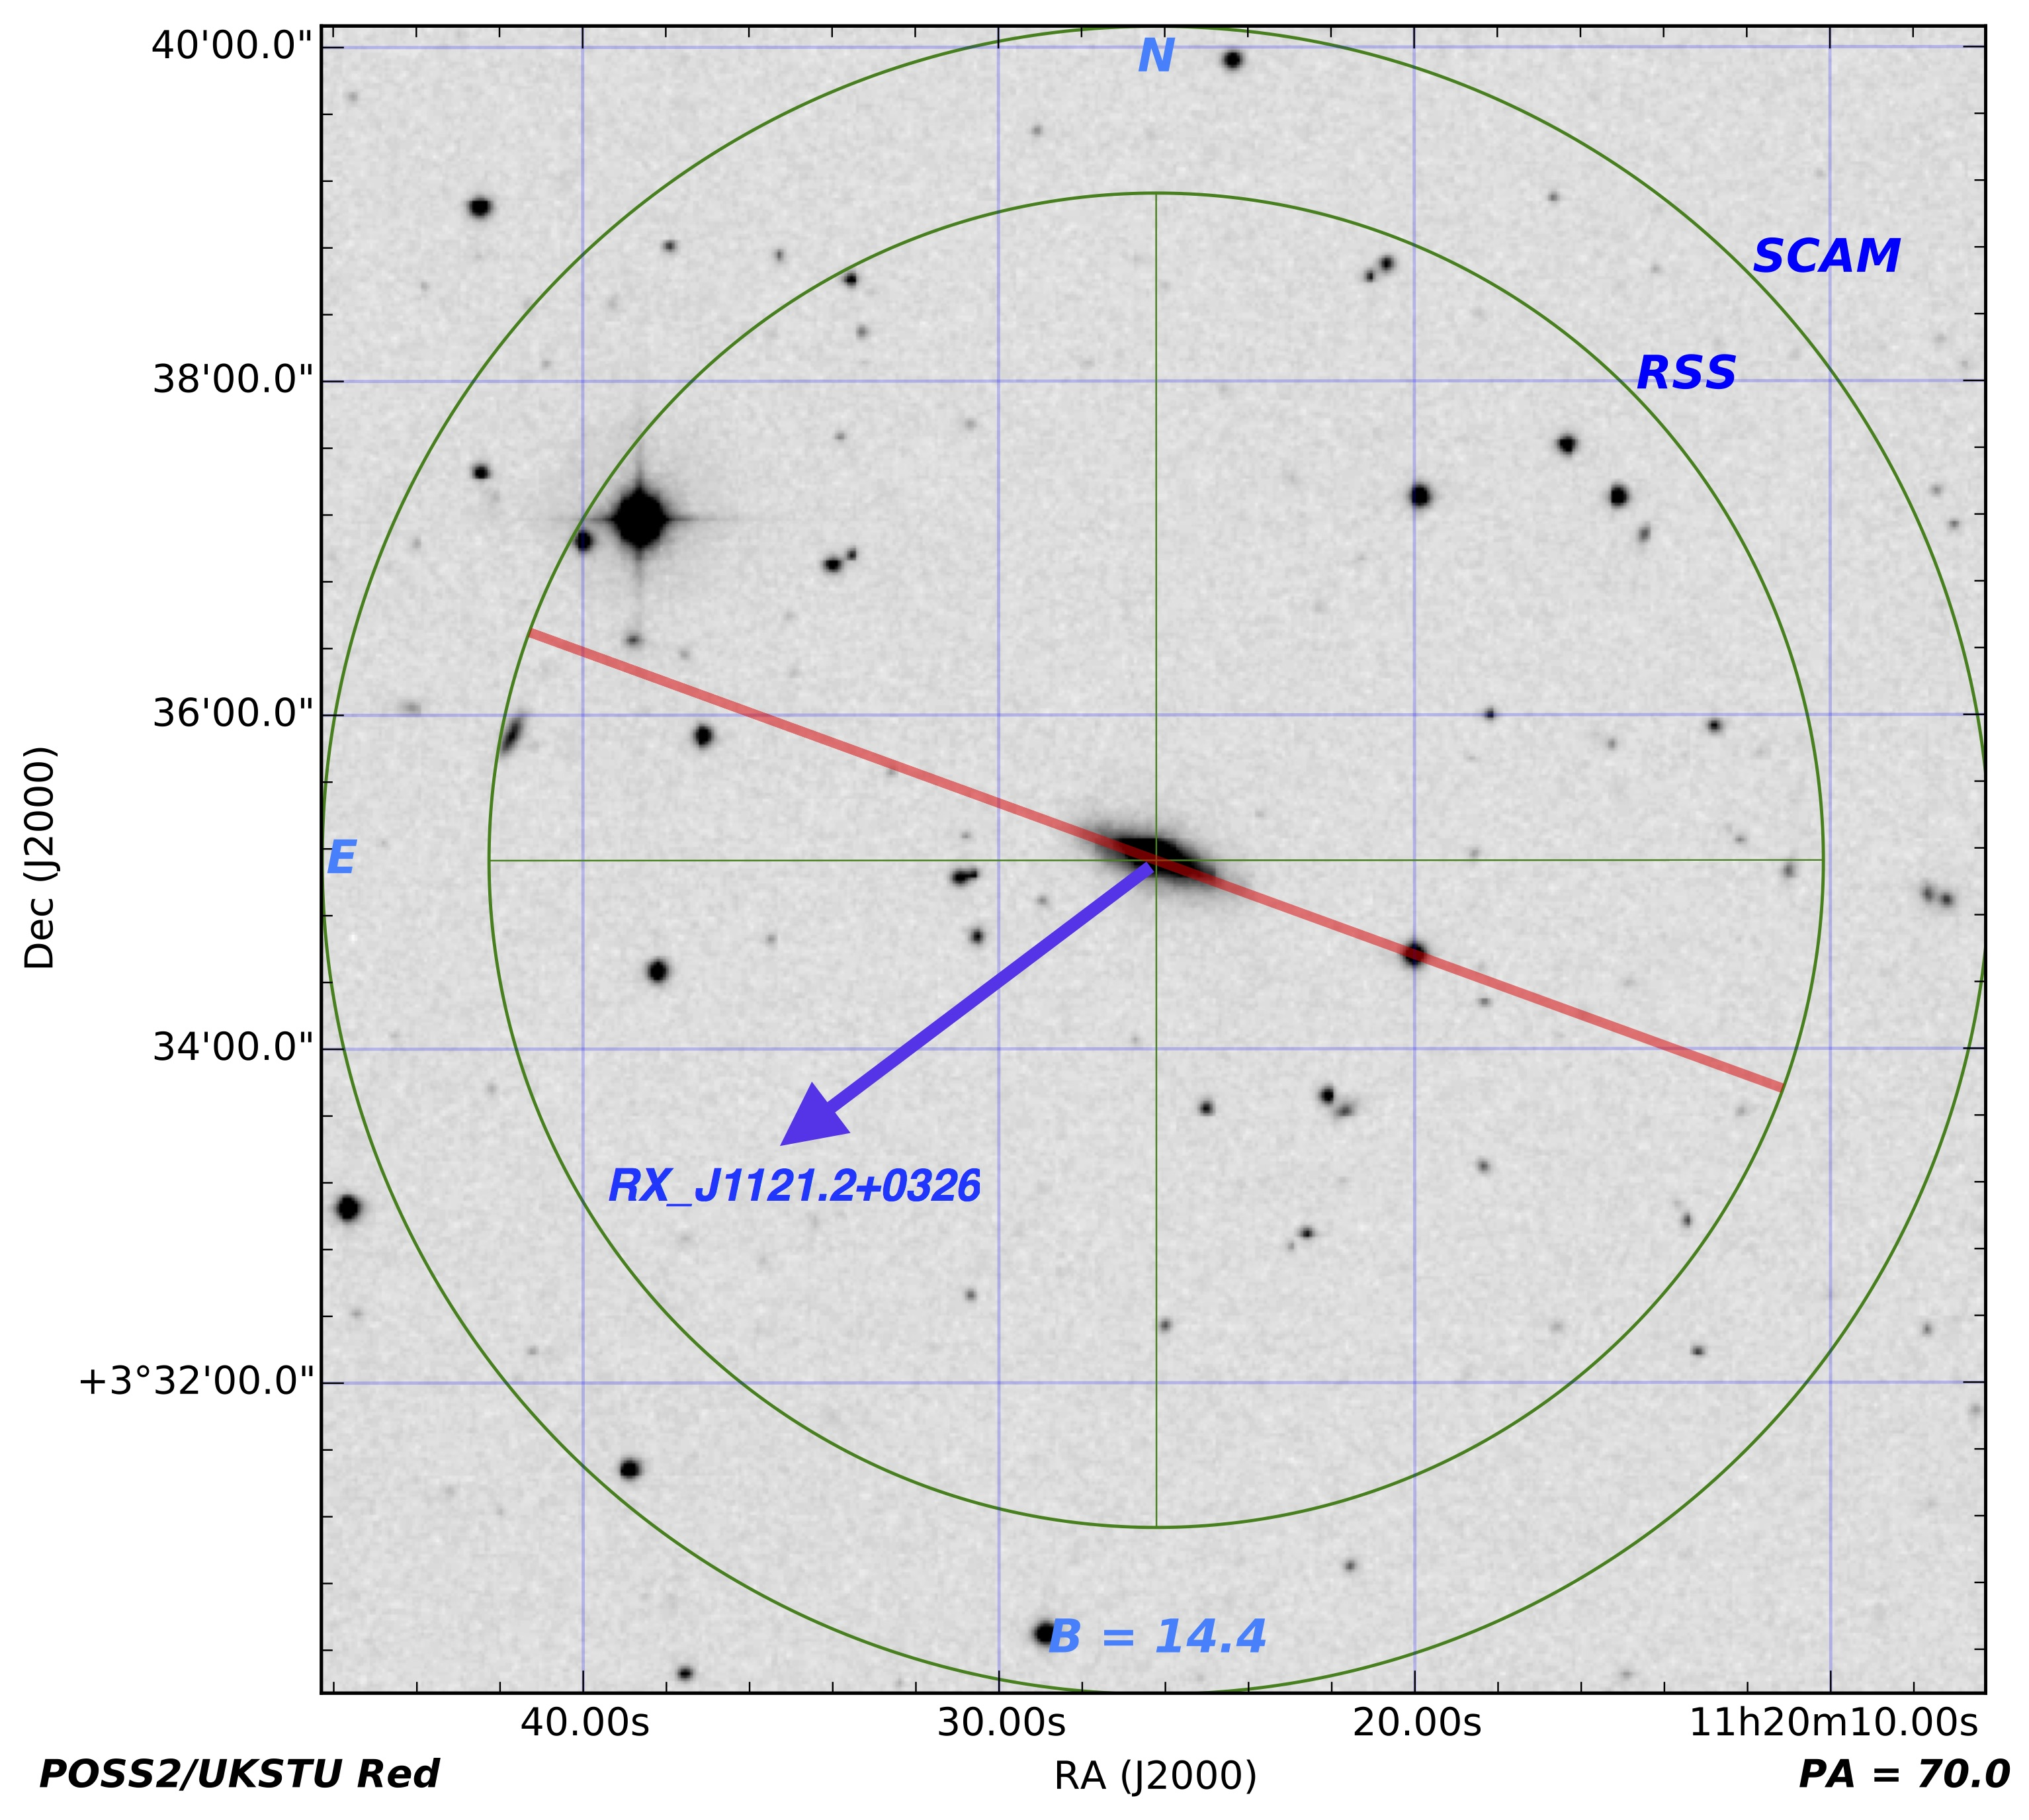
\includegraphics[width=0.45\linewidth]{Chap4/figures/NGC3633_FindingChart.jpg}\label{finderchart_NGC3633}}
  \caption{\small{a) Rotation curve of NGC4536. The solid green line indicates the weighted mean velocity over the corresponding x-axis region, and the shaded green indicates the 1$\sigma$ error in the mean. b) SALT finder chart for NGC3633 showing the position of the slit in red.}}
\vspace{0pt}
\end{figure}


%There are three nearby sightlines: SDSSJ112005.00+ 041323.0 is straight north at 468 kpc and $78^{\circ}$ azimuth, RX\_J1121.2+0326 is to the southeast at 184 kpc and $58^{\circ}$ azimuth, and SDSSJ112224.10+031802.0 at 413 kpc and $50^{\circ}$ azimuth. 

%Toward RX\_J1121.2+0326 we detect a Ly$\alpha$ absorber at 2605 \kms~on the approaching side, which is essentially systemic velocity for NGC3633. The spectrum of SDSSJ112224.10+031802.0 shows absorbers at 2285 and 2578 \kms, both of which are of the correct sign for co-rotation. We do not detect any Ly$\alpha$ towards the third sightline, SDSSJ112224.10+031802.0.

%SDSSJ112005.00+041323.0 and SDSSJ112224.10+ 031802.0 are both outside of our 2 x 3 $R_{vir}$ model limits. 



\subsection{NGC4536}
NGC4536 is a SAB(rs)bc type galaxy located in the Virgo Cluster at a measured systemic velocity of $v_{sys} = 1867 \pm 33$ \kms~and inclination $i = 61^{\circ}$. The data on the receding side of NGC4536 is quite messy, and may include contamination from background sources. Hence, our measured systemic velocity, and thus rotation velocity of $139 \pm 37$ \kms, have relatively high uncertainty. Other published redshift values available from NED and rotation velocities from the HyperLEDA database are broadly consistent with our values, albeit biased slightly lower and higher in velocity, respectively.

There are 2 sightlines to the southwest of NGC4536, both on the receding side of the galaxy. HE1228+0131 at $ \rho = 338$ kpc and $86^{\circ}$ azimuth has 5 Ly$\rm \alpha$ lines: $v_{\rm Ly\alpha} =$ 1495, 1571, 1686, 1721, 1854 \kms~($\Delta v = -$372, -296, -181, -146, -13 \kms). None of these are of the correct orientation for co-rotation relative to our model predictions (cylindrical = [18, 51], NFW = [2, 32] \kms), and all are more likely to be associated with other nearby galaxies, such as NGC4517A, which is slightly closer to these absorbers in impact parameter and velocity than is NGC4536. At $v_{\rm Ly\alpha}  = 1686$ \kms~we also detect C\,{\sc ii}, C\,{\sc iv}, Si\,{\sc ii}, Si\,{\sc iii}, and Si\,{\sc iv}, and at $v_{\rm Ly\alpha}  = 1721$ \kms~we detect Lyman series from Ly$\rm \alpha$ to Ly$\rm \theta$ as well as C\,{\sc ii}, C\,{\sc iii}, C\,{\sc iv}, Si\,{\sc ii}, Si\,{\sc iii}, and Si\,{\sc iv}.

The second nearby sightline is toward 3C273 at $\rho = 344$ kpc and $46^{\circ}$ azimuth angle, and shows 3 Ly$\rm \alpha$ lines at $v_{\rm Ly\alpha} =$ 1580, 2156, 2267 \kms~($\Delta v = -$287, 289, 400 \kms). Two of these are correctly oriented for co-rotation relative to our model predictions (cylindrical = [87, 121], NFW = [5, 41] \kms), but are too high in velocity to make this scenario probable. Overall, given the number of nearby galaxies and their locations, we would expect these absorbers to trace the overall velocity field instead of the halo rotation of any particular galaxy. After this galaxy was included in the SALT observing queue we realized it is actually located in the Virgo cluster, so we have decided to remove it from the statistical sample in this paper but present the observed data here nonetheless.

\begin{figure}[h!]
\centering
  \subfigure[]{\includegraphics[width=.54\linewidth]{Chap4/figures/NGC4536_2_rotation_curve_xphys_helio_vobs_vrotObs_new4.pdf}}{\label{rotationcurve_NGC4536}}
  \subfigure[]{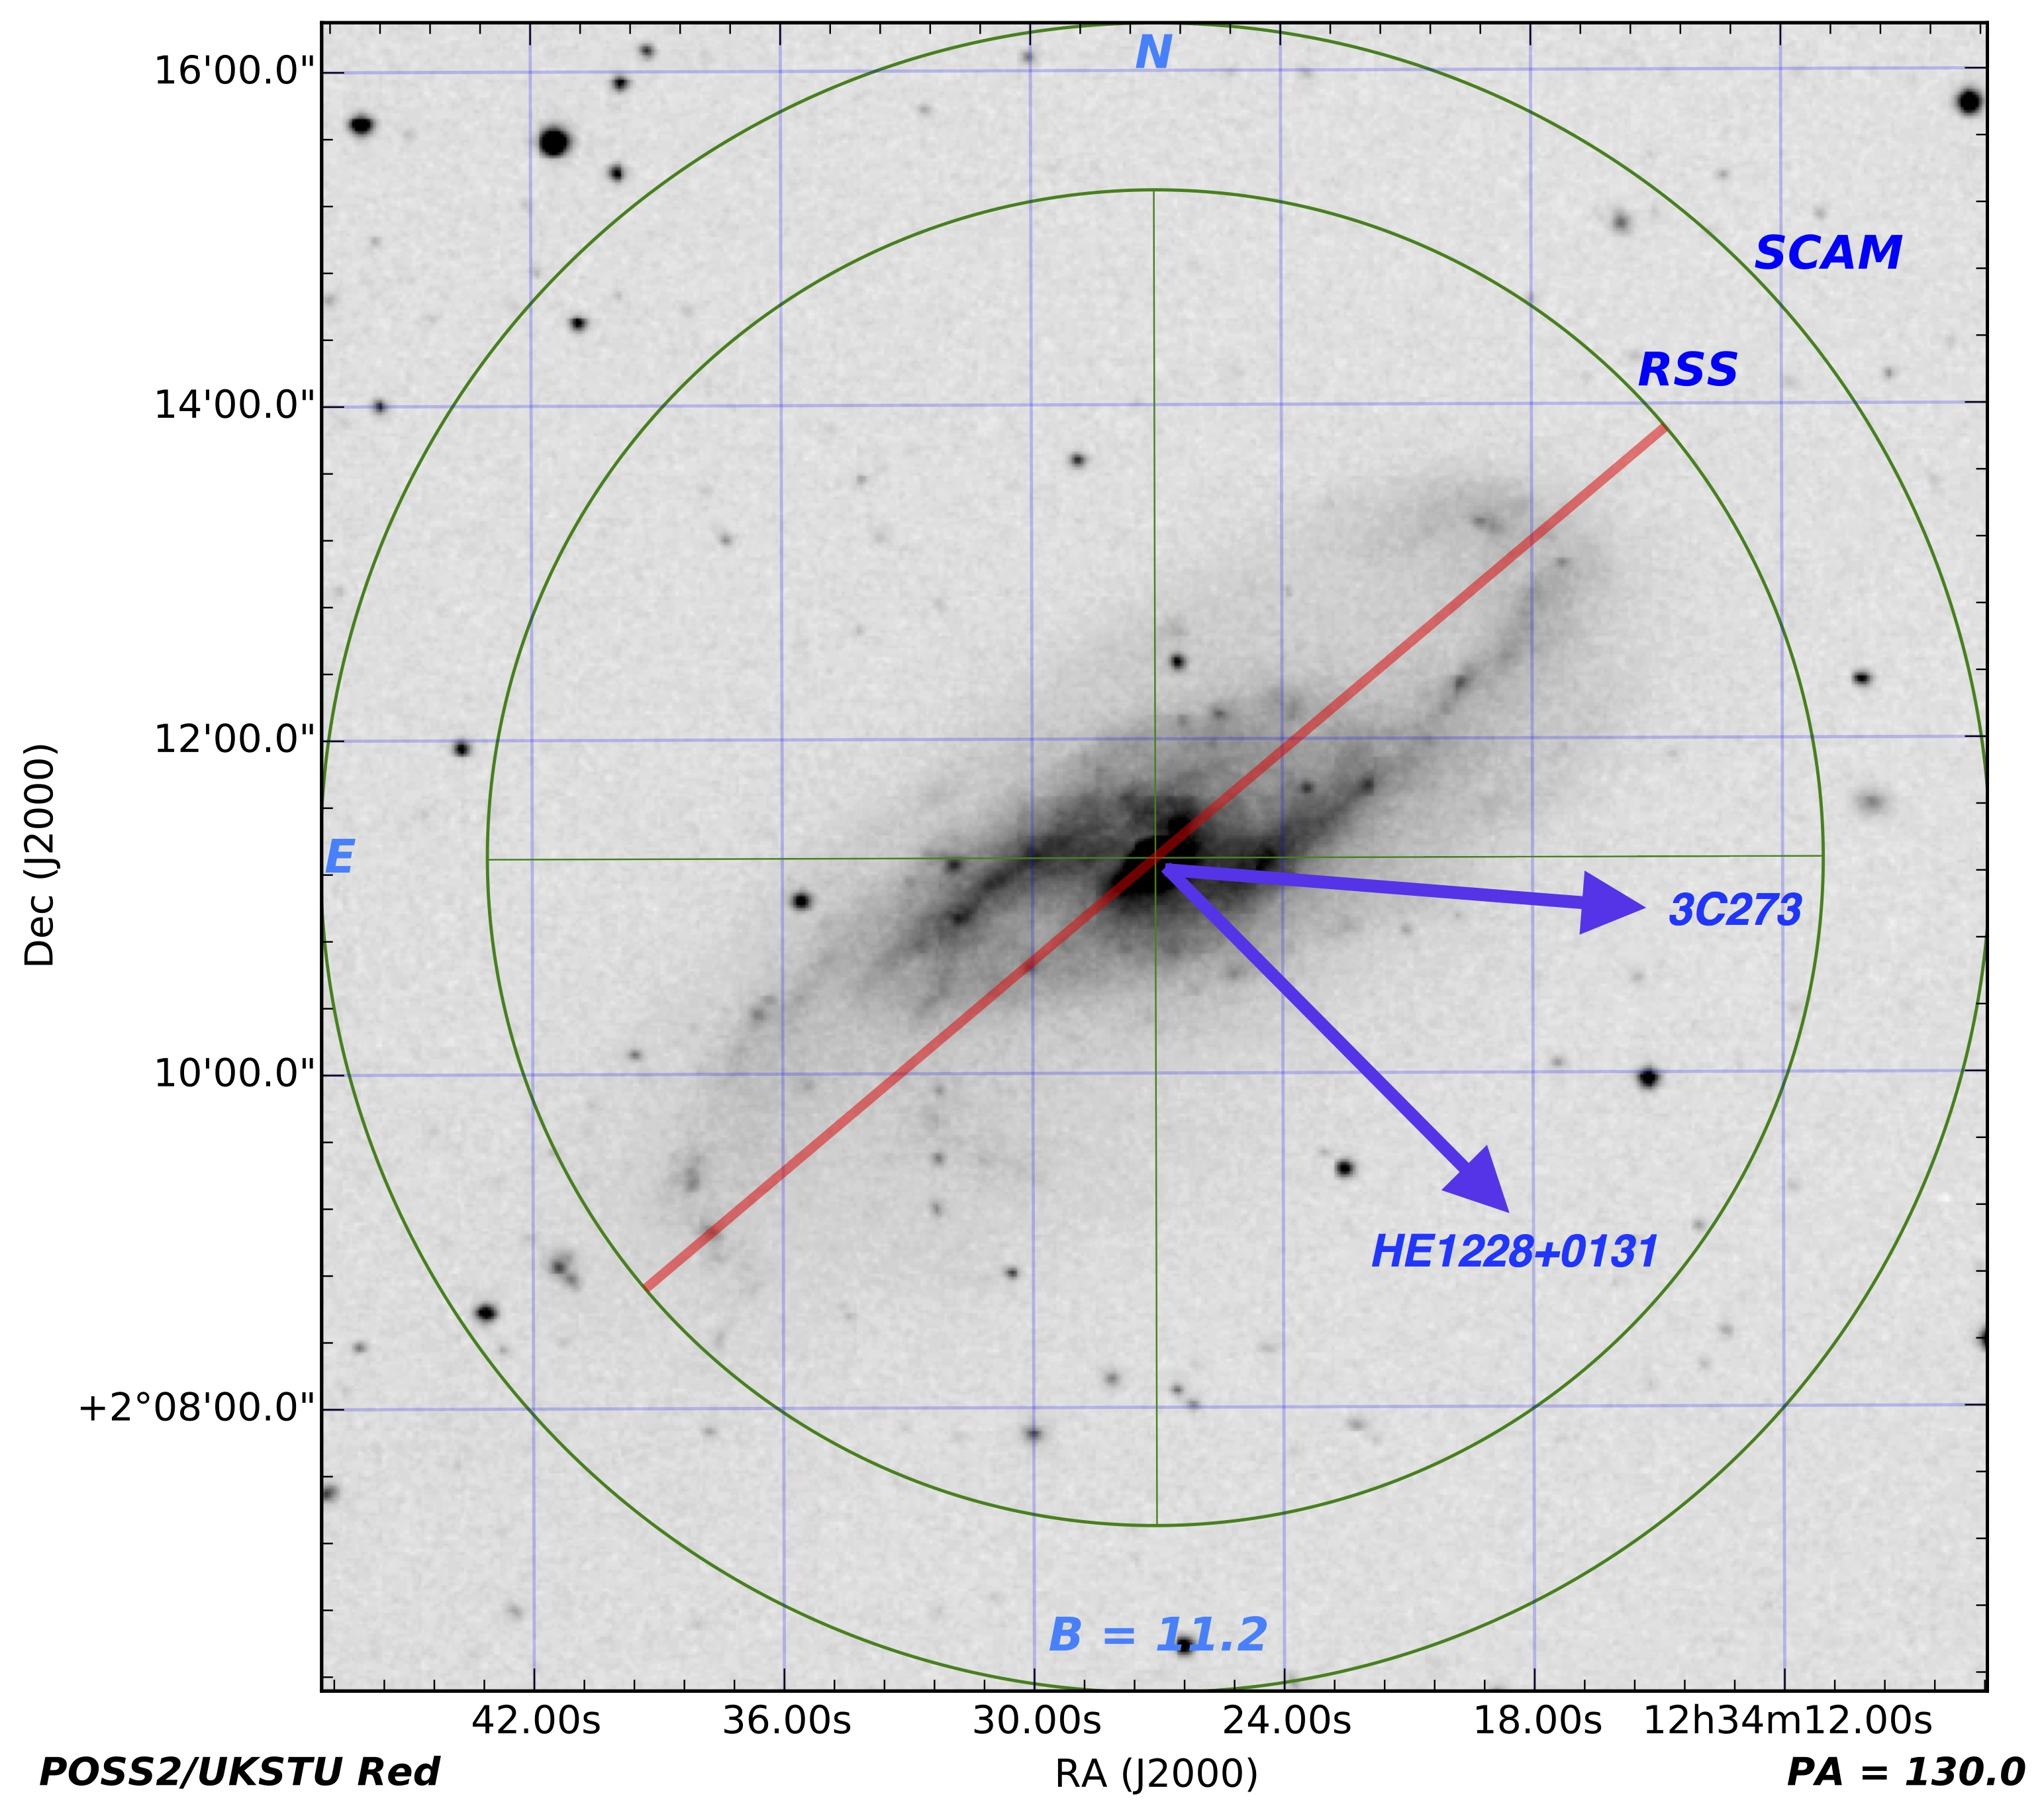
\includegraphics[width=0.45\linewidth]{Chap4/figures/NGC4536_FindingChart.jpg}\label{finderchart_NGC4536}}
  \caption{\small{a) Rotation curve of NGC4536. The solid green line indicates the weighted mean velocity over the corresponding x-axis region, and the shaded green indicates the 1$\sigma$ error in the mean. b) SALT finder chart for NGC4536 showing the position of the slit in red.}}
\vspace{0pt}
\end{figure}


%\textit{Just remove this target entirely? Or leave this discussion in place and not include it in the statistics? In this draft I have removed it entirely from the results.}

%However, the approaching side is well sampled and stable with a value of $v_{rot}=-75pm9$ \kms. For this reason, and assuming symmetry for this grand-design spiral galaxy, we have decided to adopt the same value for the receding side, $v_{rot}=75pm9$ \kms.

% The image of this galaxy is confusing - it looks opposite, because we're 'underneath' it (i.e. the near edge is up, the far edge is away). 


\subsection{NGC4939}
NGC4939 is a large SA(s)bc type galaxy with measured systemic velocity $v_{\rm sys} = 3093 \pm 33$ \kms~and inclination $i = 48^{\circ}$. The background QSO PG1302-102 is located southeast at $\rho = 254$ kpc and $61^{\circ}$ azimuth angle on the approaching side of NGC4939. We detect a Ly$\rm \alpha$ absorber at $v_{\rm Ly\alpha} = 3448$ \kms~($\Delta v = 355$\kms) towards PG1302-102. As this absorber is located on the approaching side, we can easily rule out co-rotation in this case. NGC4939 does not have any close neighbors, so represents an intriguing case against co-rotation for gas past $1 R_{\rm vir}$.

\begin{figure}[ht!]
\centering
  \subfigure[]{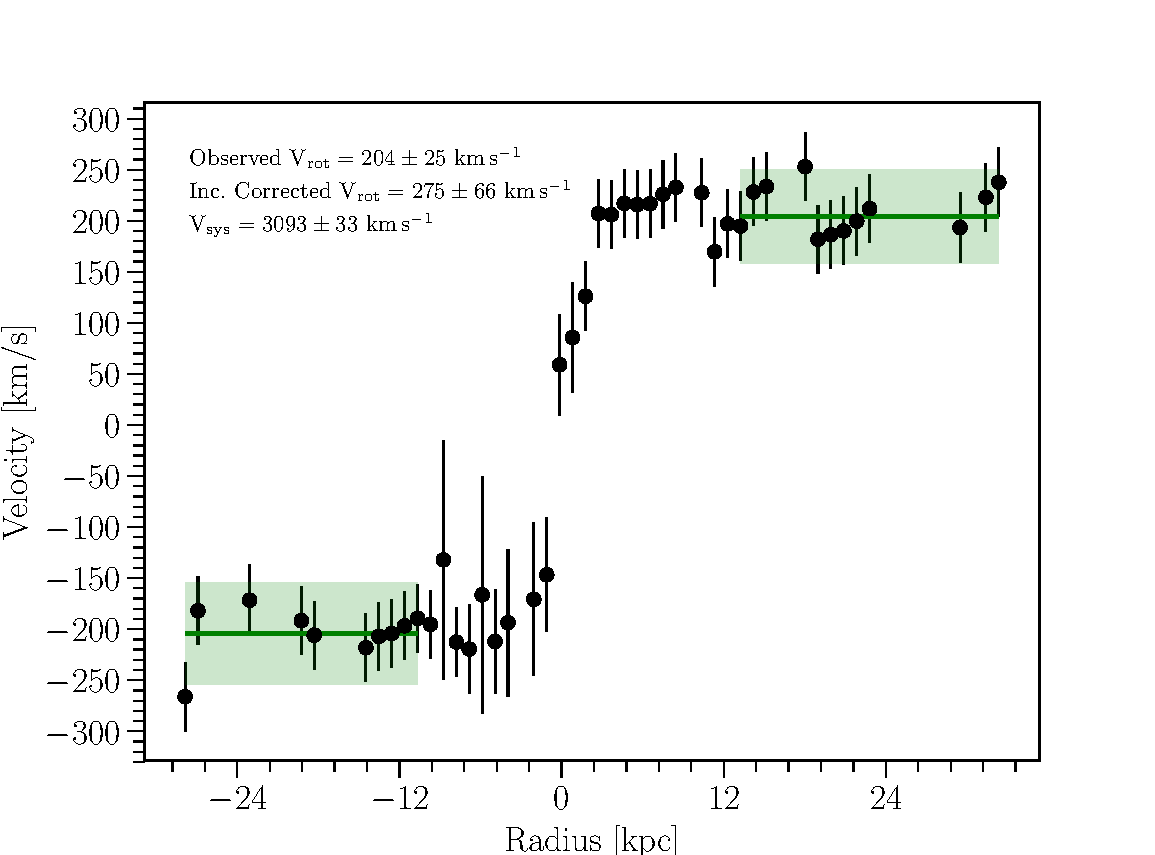
\includegraphics[width=.54\linewidth]{Chap4/figures/NGC4939_2_rotation_curve_xphys_helio_vobs_vrotObs_new4.pdf}}{\label{rotationcurve_NGC4939}}
  \subfigure[]{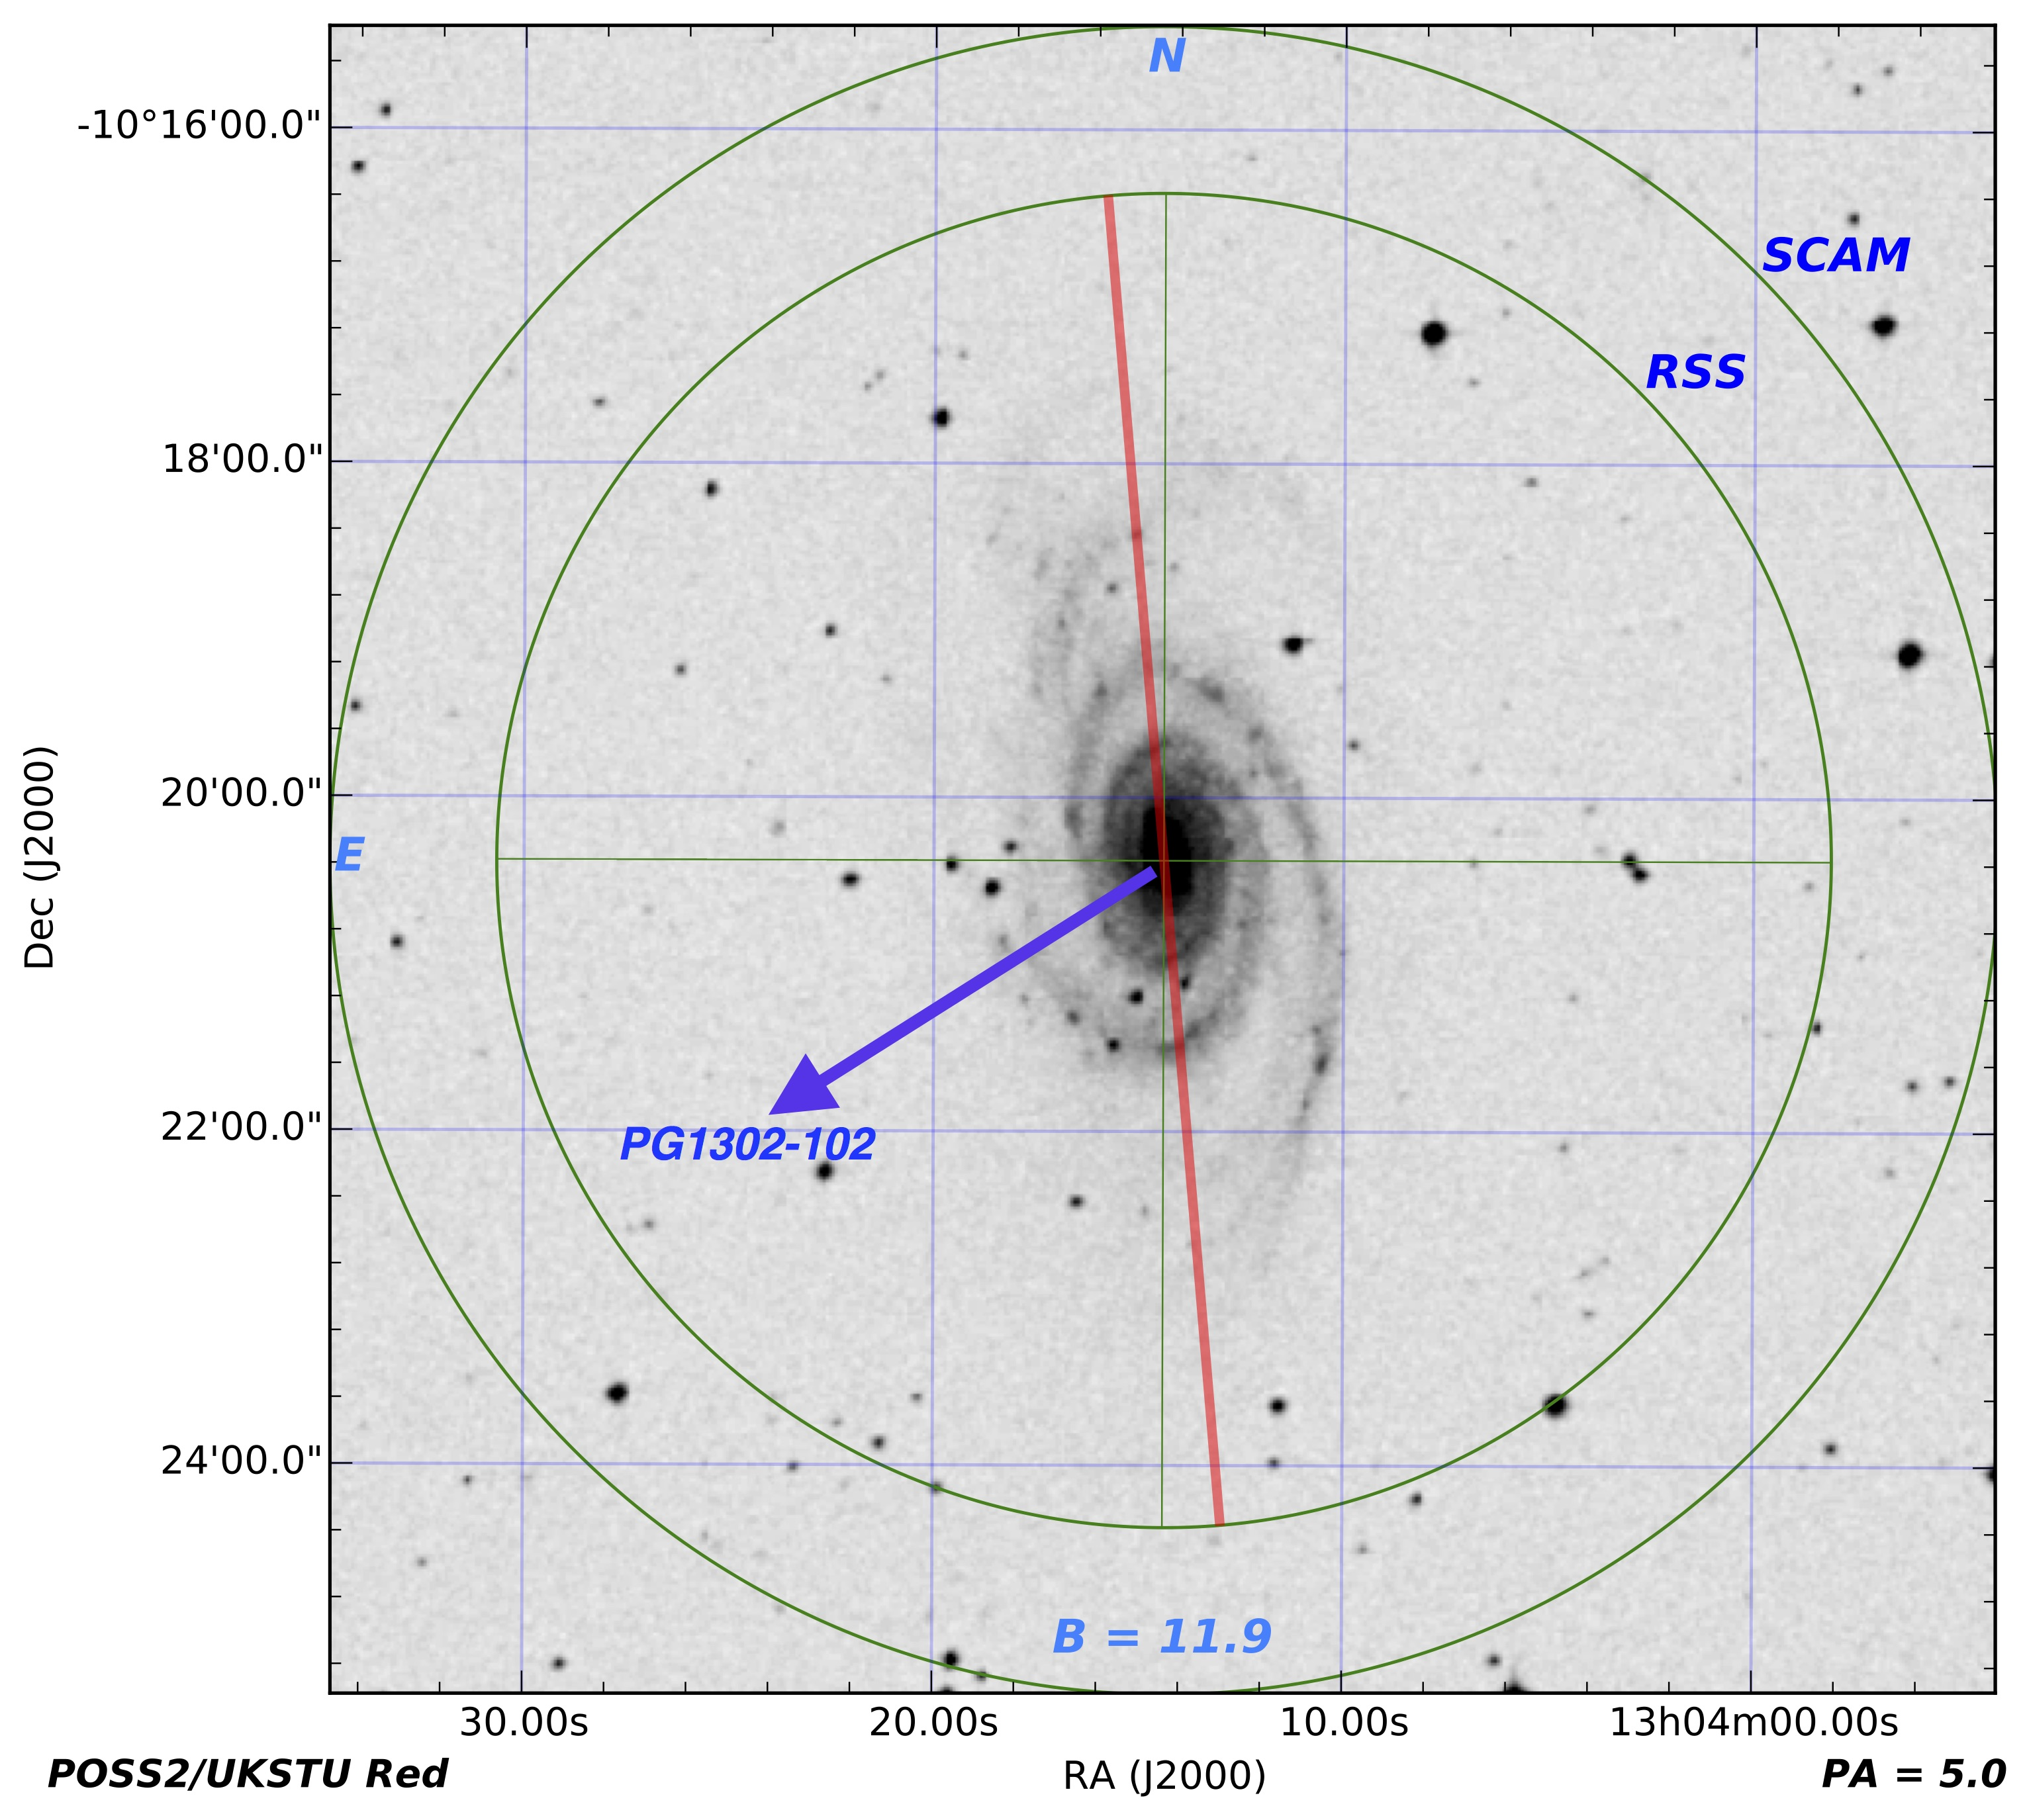
\includegraphics[width=0.45\linewidth]{Chap4/figures/NGC4939_FindingChart.jpg}\label{finderchart_NGC4939}}
  \caption{\small{a) Rotation curve of NGC4939. The solid green line indicates the weighted mean velocity over the corresponding x-axis region, and the shaded green indicates the 1$\sigma$ error in the mean. b) SALT finder chart for NGC4939 showing the position of the slit in red.}}
\vspace{0pt}
\end{figure}


\subsection{NGC5364}
NGC5364 is a SA(rs)bc pec type galaxy at a measured systemic velocity $v_{\rm sys} = 1238 \pm 17$ \kms~and inclination $i = 57^{\circ}$. It is located in a group environment with 5 other large, nearby galaxies. The background QSO SDSSJ135726.27+043541.4 is located southeast at $\rho = 165$ kpc and $84^{\circ}$ azimuth angle on the receding side of NGC5364. We detect Ly$\rm \alpha$ at $v_{\rm Ly\alpha} = 967, 1124$ \kms~($\Delta v = -271, -114$ \kms) toward SDSSJ135726.27+043541.4. These absorbers have the opposite sign for co-rotation relative to our model predictions (cylindrical = [-26, 108], NFW = [-30, 68] \kms). However, because of the orientation of NGC5364 on the sky with respect to this sightline, these absorbers lie extremely close to the inflection point were projected rotation velocities flip to approaching instead of receding. For example, shifting the location of SDSSJ135726.27+043541.4 east by a tenth of a degree ($\sim 20$ kpc) is sufficient to put these absorbers on the approaching side of NGC5364. Hence, both of these absorbers could be co-rotating with NGC5364 given very reasonable assumptions on the shape of an extended disk. Nonetheless, the fact that this system lives in galaxy group environment likely dominates the surrounding velocity field.
\begin{figure}[ht!]
\centering
  \subfigure[]{\includegraphics[width=.54\linewidth]{Chap4/figures/NGC5364_2_rotation_curve_xphys_helio_vobs_vrotObs_new4.pdf}}{\label{rotationcurve_NGC5364}}
  \subfigure[]{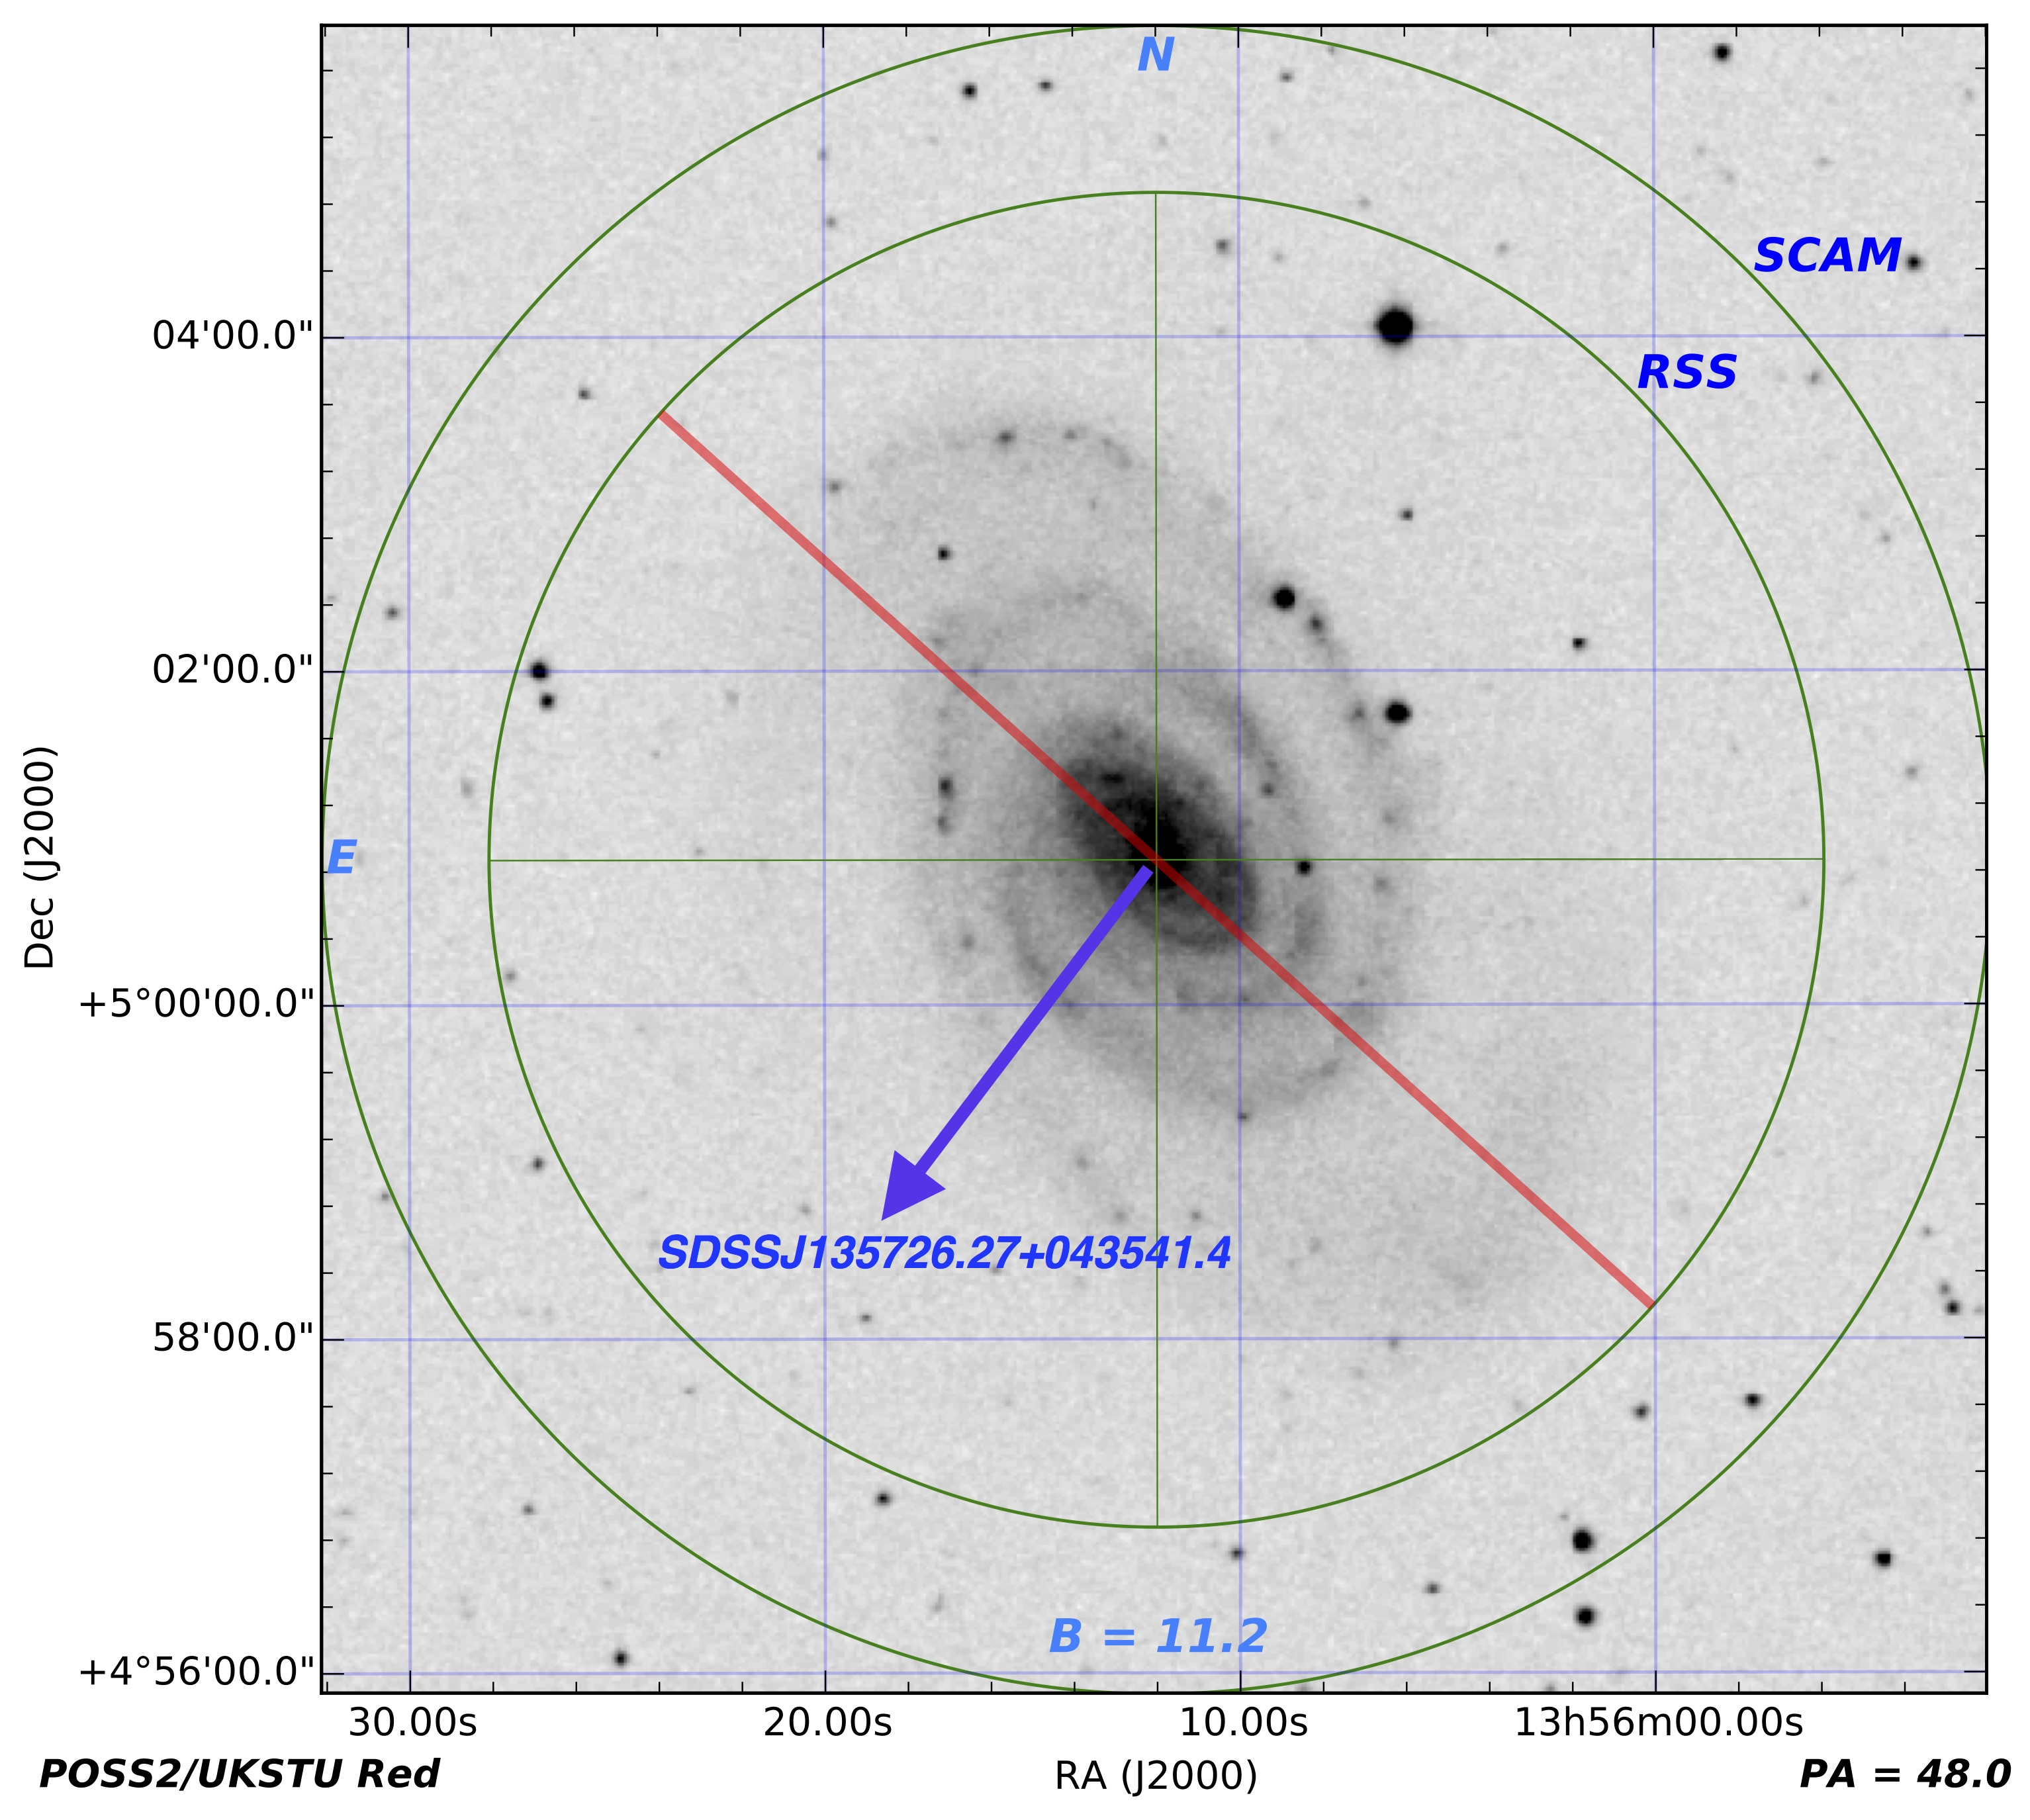
\includegraphics[width=0.45\linewidth]{Chap4/figures/NGC5364_FindingChart.jpg}\label{finderchart_NGC5364}}
  \caption{\small{a) Rotation curve of NGC5364. The solid green line indicates the weighted mean velocity over the corresponding x-axis region, and the shaded green indicates the 1$\sigma$ error in the mean. b) SALT finder chart for NGC5364 showing the position of the slit in red.}}
\vspace{0pt}
\end{figure}


\subsection{NGC5786}
NGC5786 is a large, strongly-barred spiral galaxy with measured systemic velocity $v_{\rm sys} = 2975 \pm 22$ \kms~and inclination $i = 65^{\circ}$. The background QSO QSO1500-4140 is located directly east at $\rho = 453$ kpc and $1^{\circ}$ azimuth angle on the receding side of NGC5786. We detect Ly$\rm \alpha$ at $v_{\rm Ly\alpha} = 3138$ \kms~($\Delta v = 163$ \kms) toward QSO1500-4140, which is slightly above the model predicted velocity range (cylindrical = [106, 160], NFW = [19, 67] \kms). However, the two neighboring galaxies ESO327-G038 and ESO327-G039 are both located south of NGC5786 at $\rho = 62, 296$ kpc, respectively. These nearby galaxies, along with the large distance to the absorption ($\sim 2.5 R_{\rm vir}$), make it difficult to believe this as evidence of an NGC5786 extended disk.

\begin{figure}[ht]
\centering
  \subfigure[]{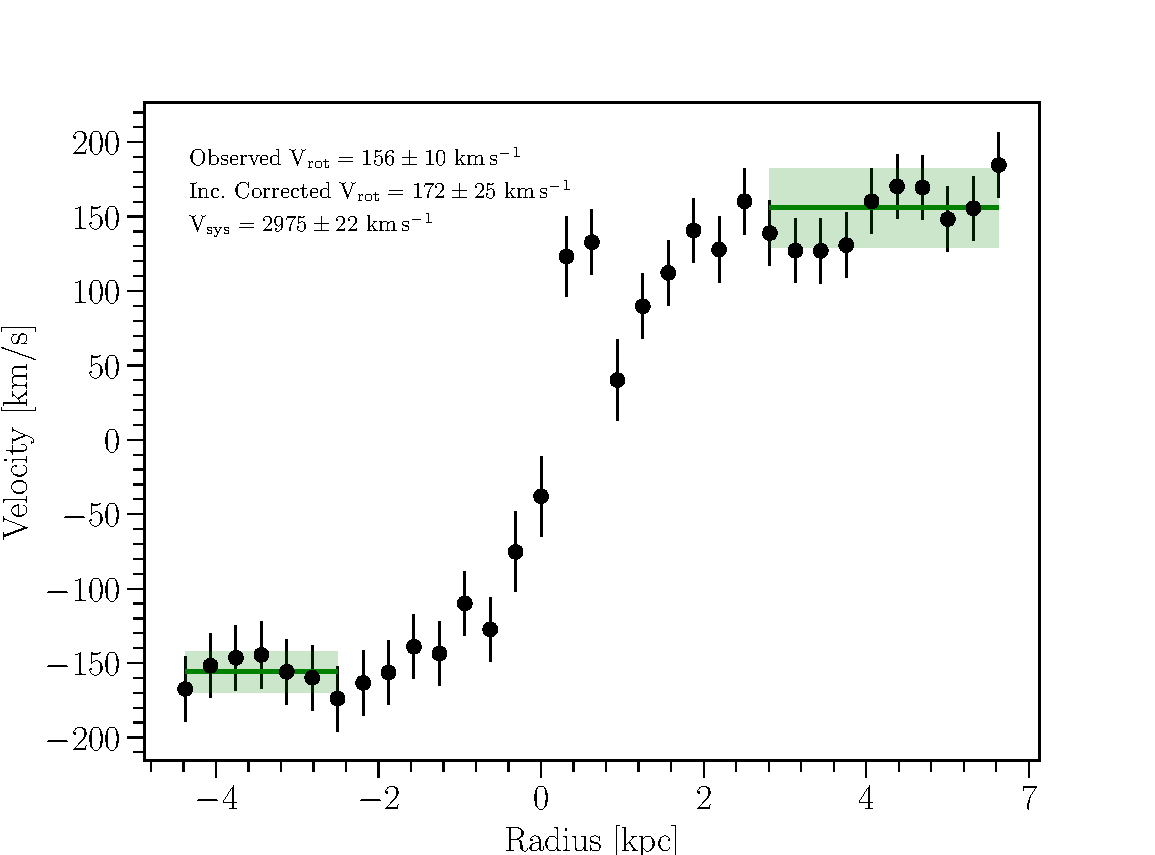
\includegraphics[width=.54\linewidth]{Chap4/figures/NGC5786_2_rotation_curve_xphys_helio_vobs_vrotObs_new4.pdf}}{\label{rotationcurve_NGC5786}}
  \subfigure[]{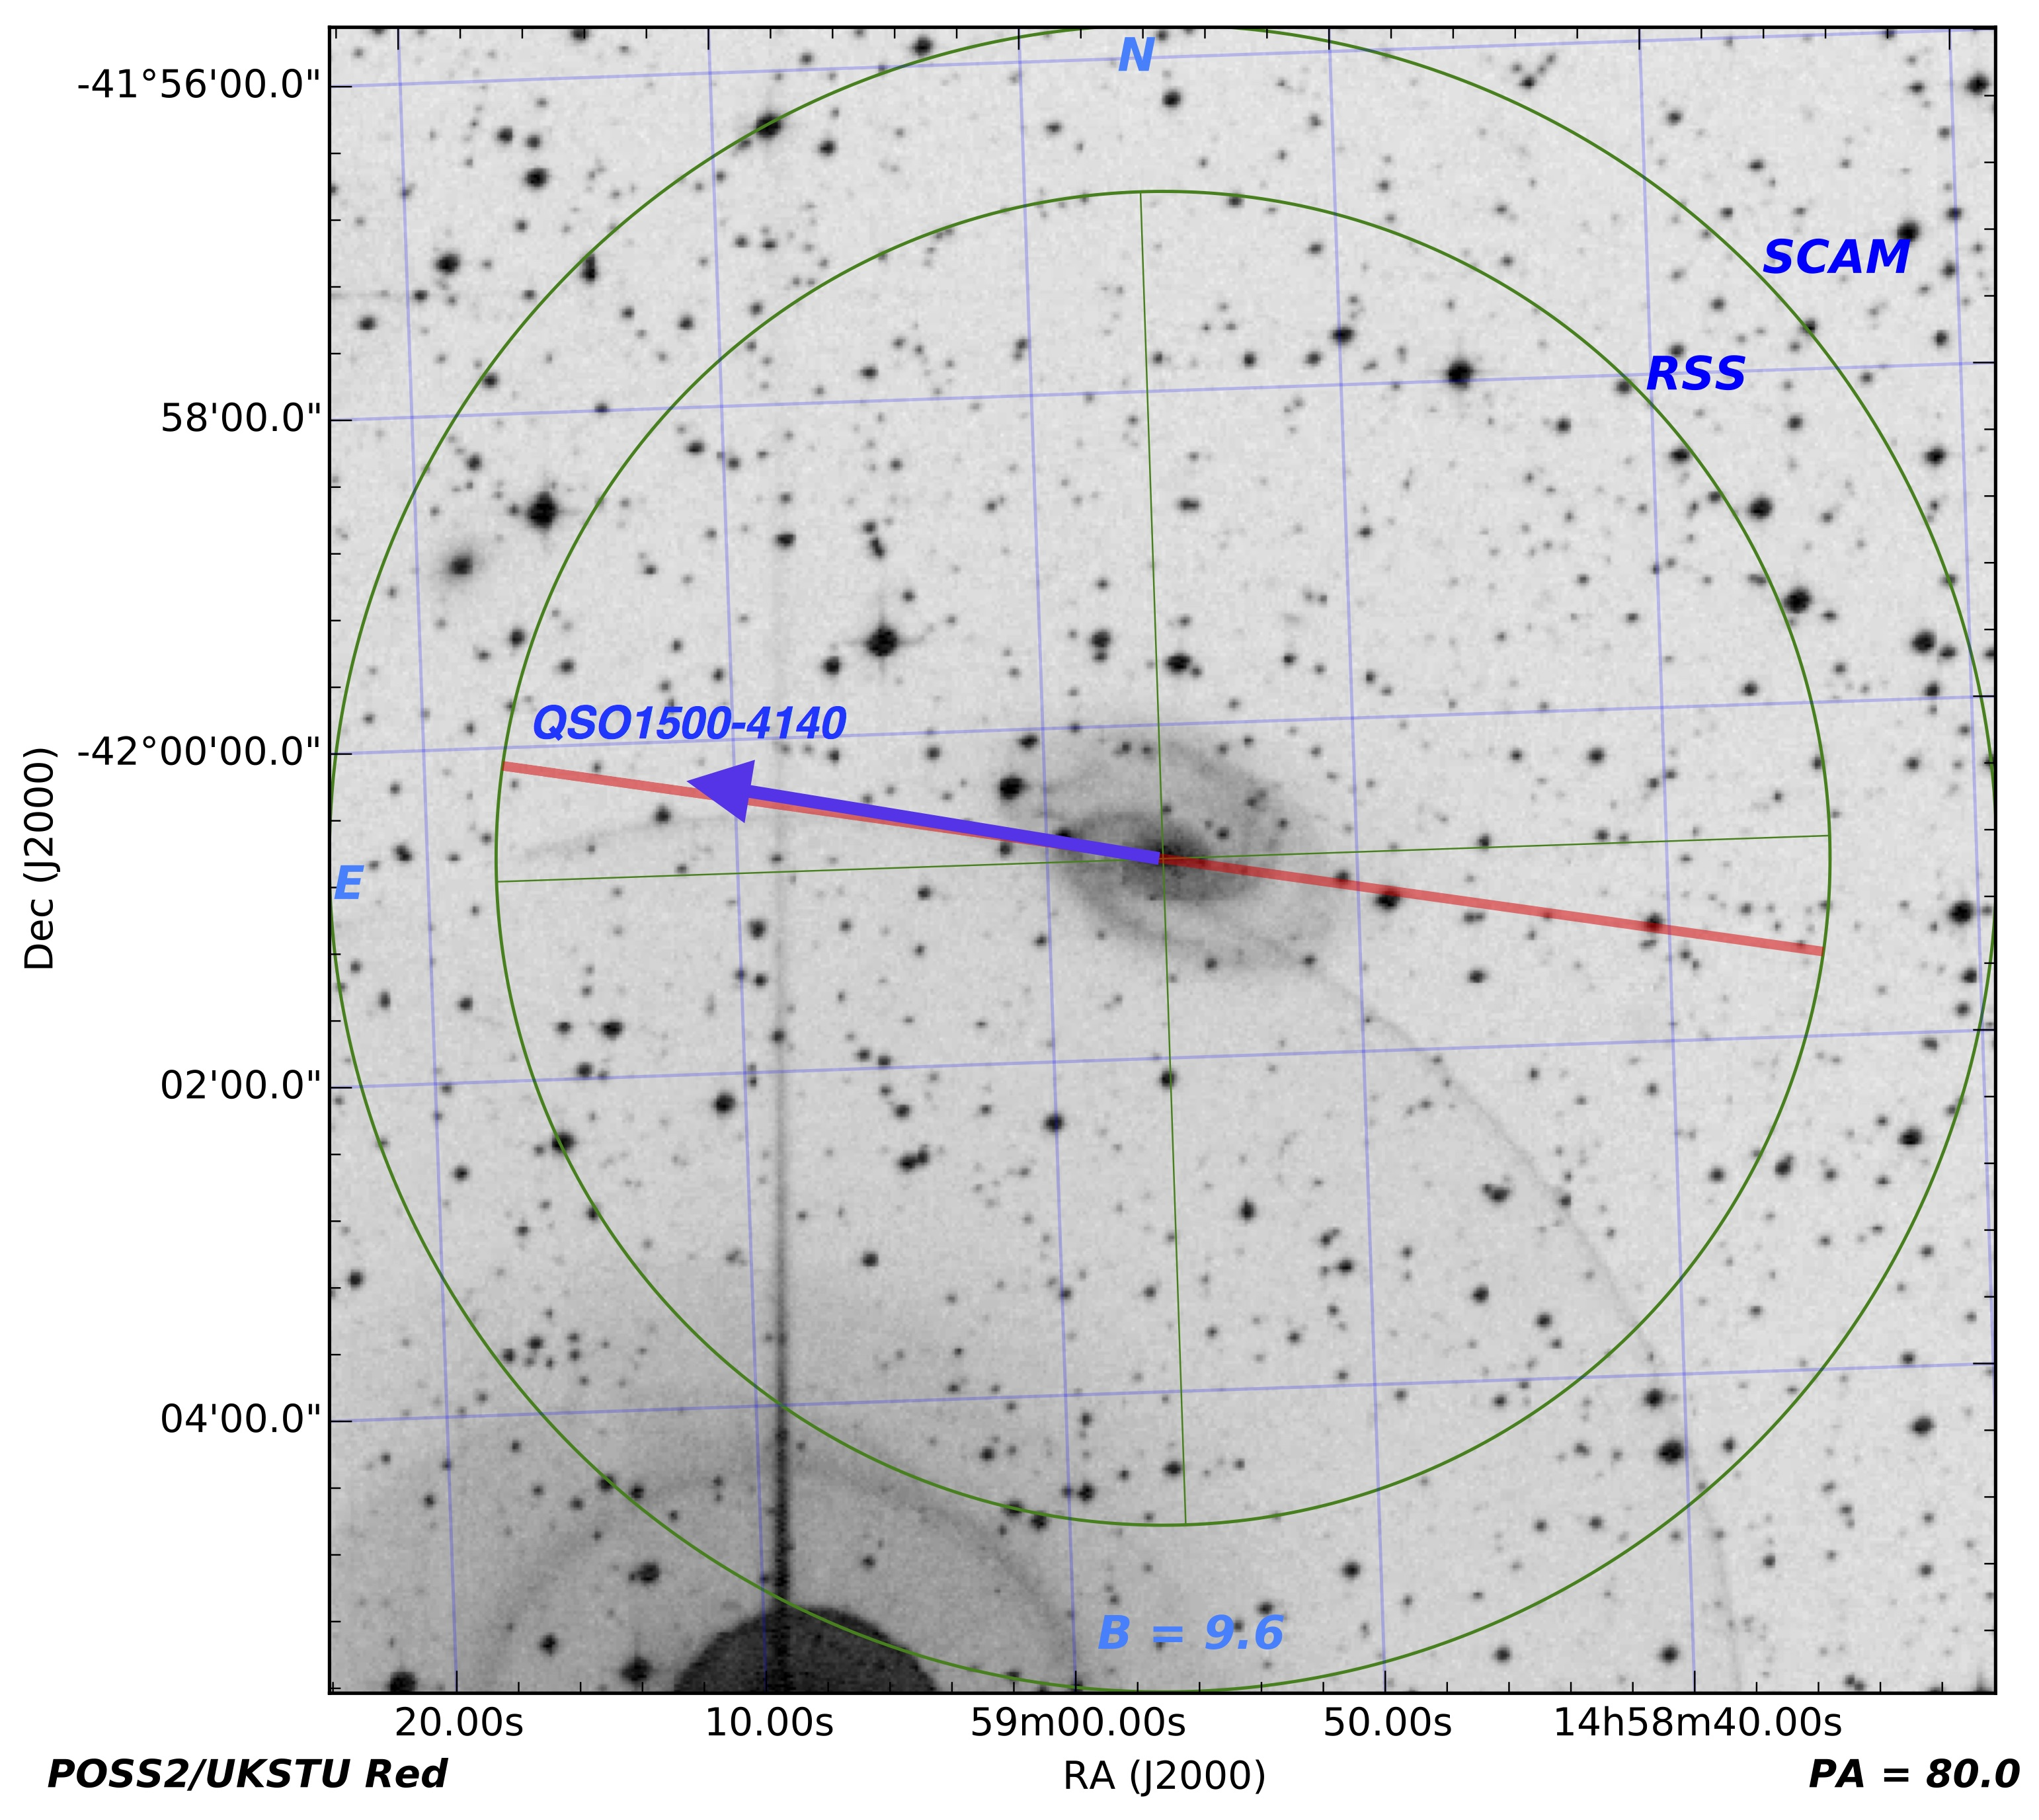
\includegraphics[width=0.45\linewidth]{Chap4/figures/NGC5786_FindingChart.jpg}\label{finderchart_NGC5786}}
  \caption{\small{a) Rotation curve of NGC5786. The solid green line indicates the weighted mean velocity over the corresponding x-axis region, and the shaded green indicates the 1$\sigma$ error in the mean. b) SALT finder chart for NGC5786 showing the position of the slit in red.}}
\vspace{0pt}
\end{figure}


\subsection{UGC09760}
UGC09760 is an edge-on, slow-rotating Sd galaxy with measured systemic velocity $v_{\rm sys} =  2094 \pm 16$ \kms. This systemic velocity deviates slightly from other published redshifts, such as the The Updated Zwicky Catalog value of $v_{\rm sys} = 2023 \pm 2$ \kms~\citep{falco1999}. This is likely due to our method of imposing rotation symmetry and averaging the approaching and receding velocities to derive $v_{\rm sys}$. If we do not sample the rotation curve far enough out, a systematic offset is not unreasonable. Indeed, we do not detect the rotation curve turnover or flattening point.

The background QSO SDSSJ151237.15+012846.0 is located southeast at $\rho = 123$ kpc and $90^{\circ}$ azimuth angle. We detect Ly$\rm \alpha$ absorption at $v_{\rm Ly\alpha} = 2029$ \kms~($\Delta v = -65$ \kms) toward SDSSJ151237.15+012846.0. This velocity falls outside the model predictions for co-rotation (cylindrical = [-30, 30], NFW = [-30, 86] \kms), but unfortunately this sightline lies almost exactly at an azimuth of $90^{\circ}$. Hence, the motion of this gas could easily be either co-rotating or counter-rotating depending on a minute change in the position angle assigned to UGC09760. This is especially true if we assume our measured $v_{sys}$ is erroneously high, and indeed closer to the values obtained by other observations. For example, if we adjust the position angle by a single degree, to $56^{\circ}$ instead of $57^{\circ}$, our model predictions become (cylindrical = [-30, 30] , NFW = [-79, 30] \kms) and this absorber becomes consistent with co-rotation in the NFW model.

%UGC09760 is an edge-on, slow-rotating Sd galaxy with a single sightline toward SDSSJ151237.15+012846.0 located 123 kpc away along the minor axis. Our measured systemic velocity,  $V_{sys} = 2094 \pm 16$, deviates slightly from other published redshifts, such as the The Updated Zwicky Catalog value of $V_{sys} = 2023 \pm 2$ \citep{falco1999}. This is likely due to our method of imposing rotation symmetry and averaging the approaching and receding velocities to derive $V_{sys}$. If we do not sample the rotation curve far enough out, a systematic offset is not unreasonable. Indeed, we do not detect the rotation curve turnover or flattening point.

It is worth noting that there are several small satellite galaxies nearby, including SDSSJ151208.16+013508.5, SDSSJ151121.63+013637.6, SDSSJ151241.38+013723.7 and UGC09746 (impact parameters $\rho = 53, 88, 82, 230$ kpc respectively). All of these galaxies lie slightly blue-ward of UGC09760, and thus \emph{farther} away in velocity from the Ly$\rm \alpha$ absorber at 2029 \kms.

\begin{figure}[ht]
\centering
  \subfigure[]{\includegraphics[width=.54\linewidth]{Chap4/figures/UGC09760_2_rotation_curve_xphys_helio_vobs_vrotObs_new4.pdf}}{\label{rotationcurve_UGC09760}}
  \subfigure[]{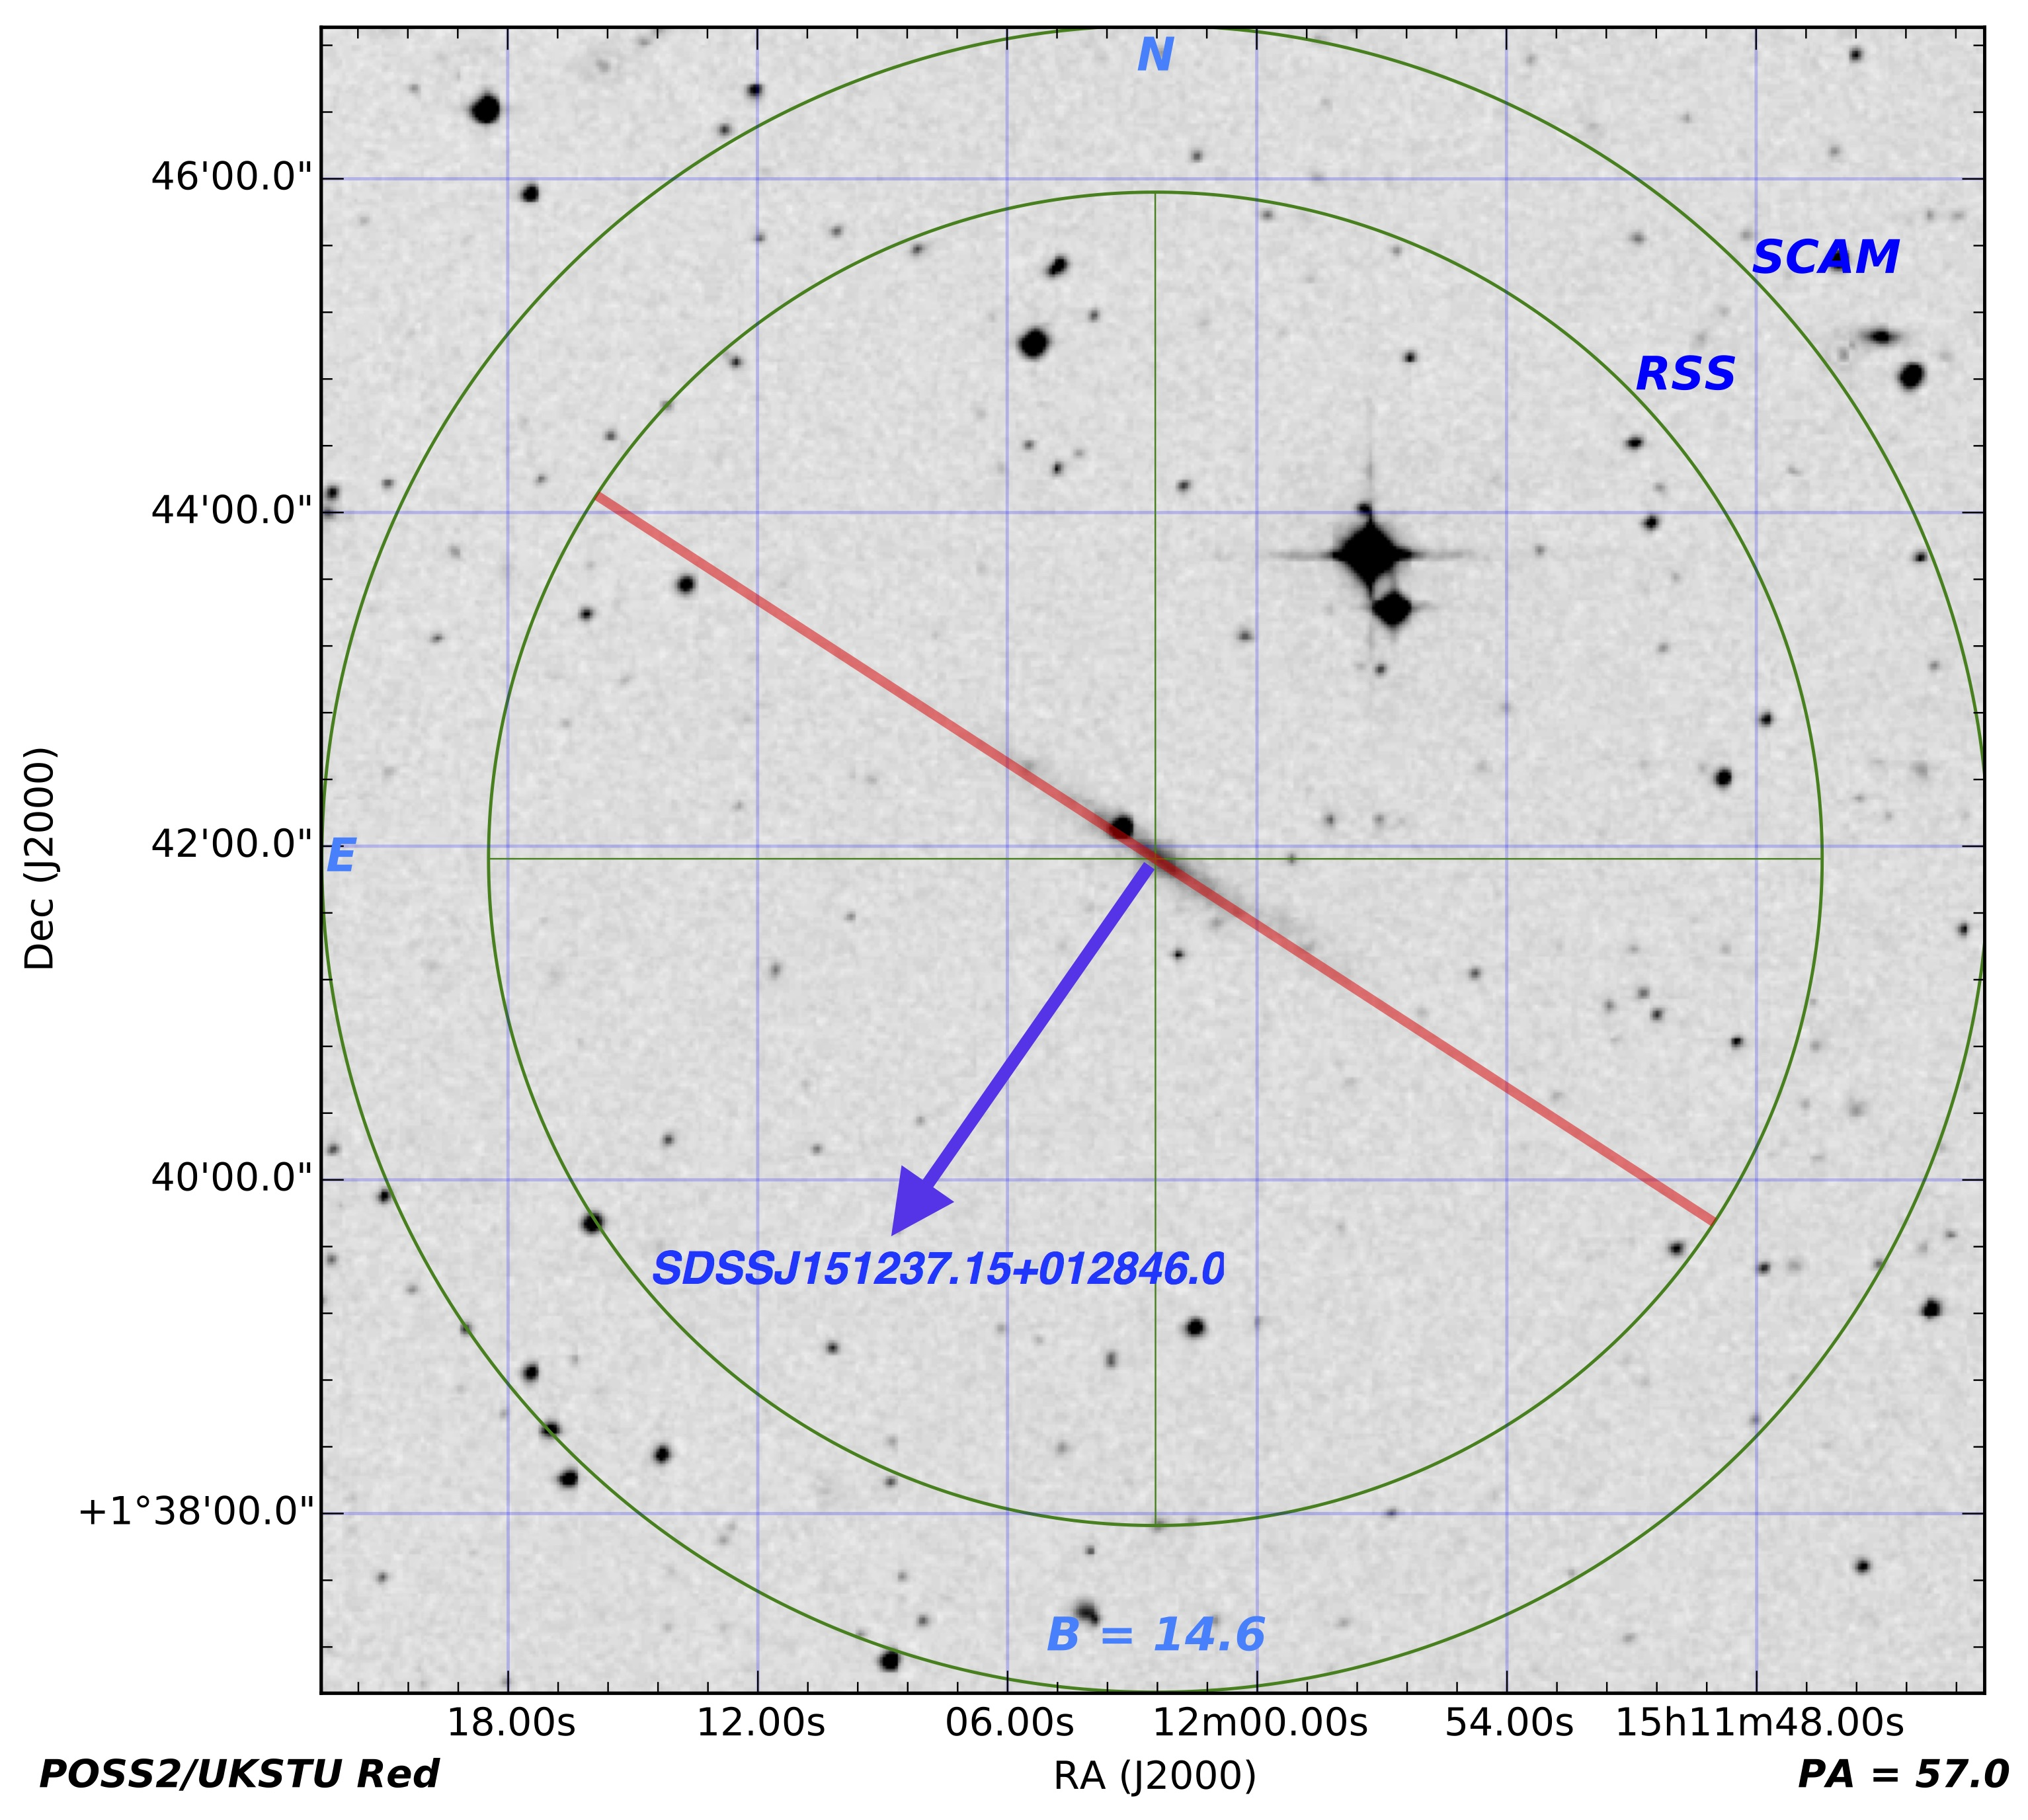
\includegraphics[width=0.45\linewidth]{Chap4/figures/UGC09760_FindingChart.jpg}\label{finderchart_UGC09760}}
  \caption{\small{a) Rotation curve of UGC09760. The solid green line indicates the weighted mean velocity over the corresponding x-axis region, and the shaded green indicates the 1$\sigma$ error in the mean. b) SALT finder chart for UGC09760 showing the position of the slit in red.}}
\vspace{0pt}
\end{figure}



\section{Ancillary Data} \label{ancillary_data}
To increase our sample size we have also searched the literature for galaxies with published rotation curves and orientations. Unfortunately, while the rotation velocity is available for thousands of galaxies, only a handful of publications also include the \emph{orientation} of the rotation on the sky. Of these, we were able to find 18 additional galaxies which have a systemic velocity greater than $\sim 500$ \kms, and are near to a COS or STIS sightline with available data. We have included 4 of the galaxy-QSO systems analyzed by \cite{cote2005}. We briefly summarize each of these systems here (see Sections \ref{NGC6140} - \ref{UGC04238}), and refer the reader to \cite{cote2005} for a more complete discussion. As new spectra and redshift-independent distances are available for these systems our results, while similar, are not identical.


%THINGS:

%\subsection{NGC0628}
%From the THINGS survey \citep{walter2008}, NGC0628 fits our criteria with a heliocentric velocity of 657 \kms~ and a sightline towards SDSSJ014143.20+134032.0 located at 377 projected kpc away. Although NGC0628 is mostly face-on ($i = 31^{\circ}$), we were able to extract a rotation curve from the publicly available THINGS first-moment \HI map.

%Heliocentric velocity = 657kms
%SDSSJ014143.20+134032.0 at 377kpc (absorption at 637, 789) - much closer to another, larger galaxy


\subsection{NGC3198}
NGC3198 is a SB(rs)c type galaxy with systemic velocity $v_{\rm sys} = 661 \pm 3$ \kms and inclination = $i = 70^{\circ}$. It is a well studied galaxy, and is included the detailed THINGS rotation curve study of \cite{deblok2008}. We extracted the raw rotation curve derived by \cite{deblok2008} using the plot digitization software WebPlotDigitizer\footnote{WebPlotDigitizer; http://arohatgi.info/WebPlotDigitizer}. NGC3198 has an even and flat rotation curve, with an average velocity of $v_{\rm rot} = 152$ \kms. The background QSO RX\_1017.5+4702 is located northeast at $\rho = 370$ kpc and $55^{\circ}$ azimuth angle on the approaching side of NGC3198. We detect Ly$\rm \alpha$ toward RX\_1017.5+4702 at $v_{\rm Ly\alpha} = 629$ \kms~($\Delta v = -32$ \kms), which can nicely be described by a co-rotating disk based on our model predicted velocity range (cylindrical = [-153, -21], NFW = [-91, 6] \kms). We note that the small dwarf galaxy SDSSJ101848.77+452137.0 is located 65 kpc away from NGC3198 toward the southwest.

%NGC3198 has an even and flat rotation curve, with an average velocity of $v_{rot} = 152$ \kms and an expected velocity range of [-82, -23] based on our projected NFW profile fit. We detect Ly$\alpha$ absorption in the spectrum of RX\_1017.5+4702 at 629 \kms ($\Delta v = -31$ \kms). Hence, the velocity of this absorber can nicely be described by a co-rotating disk.

%\textbf{SDSSJ101622.60+470643.0 is also located in the same direction but at a more distant 401 kpc away (\textbf{NOT IDENTIFIED}).}


% SDSSJ101950.83+453208.0, SDSSJ101958.45+453341.6, SDSSJ101946.39+453104.7 are PofG in the table

% (see e.g., \cite{begeman1989})
%Heliocentric velocity = 660kms - Begeman 1987, THINGS de Blok paper
%SDSSJ102152.30+464515.0 at 300kpc low res only
%RX_J1017.5+4702 at 370kpc, 55.3 azimuth (line at 629kms) = good
%SDSSJ102839.10+450009.0 at 390kpc (low res only)
%SDSSJ101622.60+470643.0 at 401kpc, 61 azimuth (no IDs, possible line) = pretty far away



\subsection{NGC3351}
NGC3351 is a mostly face-on ($i = 29^{\circ}$) SB(r)b type galaxy with systemic velocity  $v_{\rm sys} = 778 \pm 4$ \kms. It is located $\sim200$ kpc southwest of the core of the Leo I group. We take the rotation curve and orientation produced by \cite{dicaire2008}. While we expect any extended disk rotation to be quickly disrupted due to the complex Leo I environment, this galaxy also has one of the closest sightlines in our sample with SDSSJ104335.90+115129.0 at $\rho = 31$ kpc and $13^{\circ}$ azimuth on the northwest, approaching side. We detect Ly$\rm \alpha$ at $v_{\rm Ly\alpha} = 717, 882, 1030$ \kms ($\Delta v = -61, 104, 252$ \kms) toward this sightline. The lowest velocity absorber agrees nicely with both models for co-rotation, while the other two are above our model predictions (cylindrical = [-99, 12], NFW = [-68, 20] \kms). We also detect multiple metal ions associated with $v_{\rm Ly\alpha} = 717$ \kms~line, including C\,{\sc ii}, N\,{\sc i}, N\,{\sc v}, O\,{\sc i}, Si\,{\sc ii}, Si\,{\sc iii}, Si\,{\sc iv}, S\,{\sc ii}, and Fe\,{\sc ii}.


%At $V_{sys} = 778$ \kms NGC3351 is a mostly face-on ($i = 29^{\circ}$) SB(r)b type galaxy located $\sim200$ kpc southwewst of the core of the Leo I group.  We take the rotation curve and orientation produced by \cite{dicaire2008}. While we expect any extended disk rotation to be quickly disrupted due to the complex Leo I environment, this galaxy also has the closest sightline of our sample with SDSSJ104335.90+115129.0 at 31 kpc and $13^{\circ}$ azimuth on the northwest, approaching side. We detect Ly$\alpha$ at 717, 882, and 1030 \kms ($\Delta v = -61, 104, 252$ \kms) toward this sightline. The lowest velocity absorber agrees nicely with both models for co-rotation, while the other two are too high in velocity. \\

%IRAS10378+1109 - no data (clobbered by LLS) \\
%3C245.0 - low res only \\
%SDSSJ105125.80+124746.0 at 371, 76 az (proprietary until 2019) \\


%SDSSJ104335.90+115129.0 at 31kpc, 13 az (Lya at 717, 882, 1030) \\

%SDSSJ104816.30+120735.0 at 198kpc, 85 az (G130M but not in reduce) \\
%SDSSJ104709.80+130454.0 at 277kpc, 47 az (G130M but not in reduce) \\
%SDSSJ104843.50+130605.0 at 317kpc, 57 az (G130M but not in reduce) \\
%SDSSJ105220.60+101751.0 at 435kcp, 39 az (not ID'd, possible line) \\ 
%SDSSJ104341.53+085558.2 at 484kpc, 18 az (G130M but not in reduce) \\


% see mazzalay2014 also



\subsection{NGC5907}
NGC5907 is a large, edge-on SA(s)c type galaxy with systemic velocity $v_{\rm sys} = 670 \pm 3$ \kms. We take the rotation curve and orientation produced by \cite{yim2014}. The background QSO SBS1503+570 is located northwest at $\rho = 413$ kpc and $47^{\circ}$ azimuth angle on the receding side of NGC5907. We detect Ly$\rm \alpha$ at $v_{\rm Ly\alpha} = 708$ \kms~($\Delta v = 38$ \kms), which falls within the model predictions for co-rotation (cylindrical = [31, 228], NFW = [-24, 101] \kms). Unfortunately there are several other nearby galaxies, the largest of which being NGC5866 (diameter $D = 20.8$ and impact parameter $\rho = 208$ kpc, versus for NGC5907 - $D = 50.6$ and $\rho = 413$ kpc). Hence, it is difficult to assign this absorber to NGC5907 alone.


%The closest sightline resides toward SDSSJ152053.59+571122.1 on the northwest (receding) side, at 286 kpc and $63^{\circ}$ azimuth.

%Sanders 1996, Allaert (2015A\&A...582A..18A) also \\
%
%NW is receding side \citep{allaert2015}. \\
%Rotation curve data from \cite{yim2014} \\
 
%SDSSJ152053.59+571122.1 at 286 kpc, 63 az (possible line around 880 \kms, messy spectrum, not ID'd) \\
%RBS1503 at 478 kpc, 63 az (no lines)



\subsection{NGC4565}
NGC4565 is an edge-on SA(s)b type galaxy with systemic velocity $v_{\rm sys} = 1230 \pm 5$ \kms. We take the rotation curve and orientation produced by \cite{sofue1996}. The background QSO RX\_J1236.0+2641 is located directly north at $\rho = 147$ kpc and $41^{\circ}$ azimuth angle on receding side of NGC4565. We detect Ly$\rm \alpha$ absorption at $v_{\rm Ly\alpha} = 1009, 1166, 1254$ \kms~($\Delta v = -221, -64, 24$ \kms) toward RX\_J1236.0+2641. Only the $v_{\rm Ly\alpha}=1254$ \kms~line is consistent with co-rotating gas relative to our model predictions (cylindrical = [-2, 246], NFW = [-30, 144] \kms). However, the presence of several other nearby galaxies (e.g., NGC4559, NGC4562) surely disrupts any possible extended disk rotation that would otherwise be detectable via sightline absorption.

% ($i = 75^{\circ}$)

%Both are consistent with counter-rotating gas, although the line at 1166 \kms is close to the allowed range of [-29, 146] \kms~for co-rotation. 


\subsection{UGC06446} \label{UGC06446}
UGC06446 is a Sd type galaxy with systemic velocity $v_{\rm sys} = 644 \pm 1$ \kms~and inclination $i = 48^{\circ}$ on the far northwest edge of the Ursa Major cluster of galaxies. We take the rotation curve and orientation information produced by \citep{verheijen2001, swaters2009}. The background QSO SDSSJ112448.30+531818.0 is located southwest at $\rho = 143$ kpc and $22^{\circ}$ azimuth angle on the receding side of UGC06446. We detect Ly$\rm \alpha$ at $v_{\rm Ly\alpha} = 664, 1019$ \kms~($\Delta v = 20, 375$ \kms). The absorber at $v_{\rm Ly\alpha} = 664$ falls well within our model predicted co-rotation range (cylindrical = [-9, 65], NFW = [-15, 61] \kms), but the absorber at $v_{\rm Ly\alpha} = 1019$ is far more likely to be associated with NGC3631 ($\rho = 86$ kpc, $v_{\rm sys} = 1156$ \kms). We therefore treat these as separate systems.


%We detect Ly$\alpha$ absorption toward two nearby QSO's, SDSSJ112448.30+531818.0 at 143 kpc and $22^{\circ}$ azimuth (Ly$\alpha$ at 664 and 1019 \kms) and RX\_J1117.6+5301 at 417 kpc and $52^{\circ}$ azimuth (Ly$\alpha$ at 685 \kms), are both located toward the southwest, receding side of UGC06446. The absorbers residing at 664 \kms~and 685 \kms both agree well with the expected velocities for co-rotating gas ([-15, 61], [25, 35]). The 1019 \kms absorber toward SDSSJ112448.30+531818.0 is most likely associated with NGC3718, which is much closer in velocity ($V_{sys}$ = 993 \kms). Interestingly, we note that the more distant absorber toward RX\_J1117.6+5301 has a larger $\Delta v$ value ($\Delta v = 40$ \kms compared to $19$ \kms). If both absorbers were strictly following the expected NFW rotation curve, we would expect the opposite, with the more distant absorber velocity approaching $V_{sys}$.


%SDSSJ112448.30+531818.0 at 143kpc, 22 az (Lya at 664kms) \\
%RX\_J1117.6+5301 at 417kpc, 52 az (Lya at 685kms) \\

%MCG9-19-073 at 179kpc - low res only \\ 
%RBS971 at 226kpc, 88 az (clobbered by huge H2 system) \\

%Check these:
%FBSJ0908 - 200kpc
%1116+523 - 400kpc


\subsection{NGC3631}
NGC3631 is a mostly face-on ($i = 17^{\circ}$) SA(s)c type galaxy with systemic velocity $v_{\rm sys} = 1156 \pm 1$ \kms. We take the rotation curve and orientation information produced by \cite{knapen1997}. There are 4 nearby QSOs, which we will present in order of increasing impact parameter.

First, the closest background QSO RX\_J1117.6+5301 is located southwest at $\rho = 78$ kpc and $75^{\circ}$ azimuth angle on the receding side of NGC3631. We detect Ly$\rm \alpha$ at $v_{\rm Ly\alpha} = 1131, 1259$ \kms~($\Delta v = -25, 103$ \kms). Both of these lines fall outside of our model predicted velocities (cylindrical = [10, 24], NFW = [1, 21] \kms).

Second, background QSO SDSSJ112448.30+531818.0 is located northeast at $\rho = 86$ kpc and $74^{\circ}$ azimuth angle on the approaching side of NGC3631. We detect Ly$\rm \alpha$ at $v_{\rm Ly\alpha} = 1019, 1141$ \kms~($\Delta v = -137, -15$ \kms). Only the higher velocity absorber falls within our model predicted velocity range (cylindrical = [-26, -11], NFW = [-22, 1] \kms).

Third, the background QSO SDSSJ111443.70+525834.0 is located in the same direction but farther than RX\_J1117.6+5301, at $\rho = 145$ kpc and $72^{\circ}$ azimuth angle on the receding side of NGC3631. We detect Ly$\rm \alpha$ at $v_{\rm Ly\alpha} = 1163$ \kms~($\Delta v = 7$ \kms). This absorber appears to agree well with our model predicted velocity range (cylindrical = [8, 29], NFW = [-5, 24] \kms).

Finally, the background QSO SBS1116+523 is located south at $\rho = 163$ kpc and $40^{\circ}$ azimuth angle on the approaching side of NGC3631, but we do not detect any Ly$\rm \alpha$ within $\pm400$ of NGC3631.

%Unfortunately, while this galaxy has 4 nearby QSOs, there are also numerous other large galaxies that are likely disturbing any extended velocity field from NGC3631. The closest of these are NGC3657 ($\rho = 75$ kpc, $D = 6.3$ kpc, $v_{\rm sys} = 1215$ \kms), and UGC06251 ($\rho = 181$ kpc, $D = 10.2$ kpc, $v_{\rm sys} = 1146$ \kms).


% Note: SDSSJ112103.68+531016.1, SDSSJ112103.92+531005.2, SDSSJ112059.33+531125.6, and SDSSJ112110.17+530951.2 are part or likely part of NGC3631.


%UGC06446 is an Sd galaxy located at $V_{sys} = 644 \pm 1$ \kms~on the far northwest edge of the Ursa Major cluster of galaxies. We take the rotation curve and orientation information from \citep{verheijen2001, swaters2009}. The background QSO SDSSJ112448.30+531818.0 is located southwest at $\rho = 143$ kpc and $22^{\circ}$ azimuth angle on the receding side of UGC06446. We detect $Ly\alpha$ at $V_{Ly\alpha} = 664, 1019$ \kms~($\Delta v = 20, 375$ \kms). The absorber at $V_{Ly\alpha} = 664$ falls well within our model predicted co-rotation range (cylindrical = [-9, 65], NFW = [-15, 61] \kms), but the absorber at $V_{Ly\alpha} = 1019$ is far more likely to be associated with NGC3631 ($\rho = 86$ kpc, $V_{sys} = 1156$ \kms). We therefore treat these as separate systems.

%Southeast side approaching

%\subsection{UGC06399}
%UGC06399 is an edge-on Sm type galaxy located at $V_{sys} = 791$ \kms~on the far west edge of the Ursa Major cluster of galaxies. Again, we take the rotation curve and orientation information from \citep{verheijen2001, swaters2009}. As noted by \cite{verheijen2001}, this is the most isolated galaxy in the Ursa Major cluster. Unfortunately, the closest QSO is SBS1116+523, at 471 kpc away on the northwest, approaching side. Although we detect Ly$\alpha$ absorption at 731 \kms, this impact parameter is beyond our model radius of $3 R_{vir}$. Nonetheless, the velocity of this absorber agrees well with the expected velocity range if we extend a static or NFW rotating disk out to $4 R_{vir}$.


%SBS1116+523 at 471kpc, 13.4 az (Lya at 731kms) \\

%MCG9-19-078 at 301kpc (G160M only) \\
% southeast side is receding


\subsection{NGC3726}
NGC3726 is a SAB(r)c type galaxy with systemic velocity $v_{\rm sys}= 866 \pm 1$ \kms~and inclination $i = 52^{\circ}$ on the southwestern edge of the Ursa Major galaxy cluster \citep{verheijen2001}. The closest background QSO, CSO1208, is located southeast at $\rho = 369$ kpc and $88^{\circ}$ azimuth angle on the receding side of NGC3726. We detect Ly$\rm \alpha$ at $v_{\rm Ly\alpha} = 731, 874$ \kms~($\Delta v = -135, 8$ \kms) toward CSO1208. Only the higher velocity absorber falls within our predicted velocity range (cylindrical = [-27, 29], NFW = [-28, 21] \kms). A more distant QSO, RX\_J1142.7+4625, is located in the same direction as CSO1208 at $\rho = 440$ kpc and $86^{\circ}$ azimuth angle on the approaching side of NGC3726. We detect Ly$\rm \alpha$ at $v_{\rm Ly\alpha} = 818$ \kms~($\Delta v = -48$ \kms), which falls just outside our predicted velocity range (cylindrical = [-34, -14], NFW = [-30, -7] \kms). 

These two QSOs lie very close to and on apposing sides of the minor axis, such that CSO1208 samples the receding side and RX\_J1142.7+4625 the approaching. Unfortunately, both are also closer to a small group of dwarf galaxies, including NGC3782 and MCG+08-21-092, $\sim 100$ \kms~blueward of NGC3726. The $v_{\rm sys} = 731$ \kms~line toward CSO1208 is likely associated with this dwarf group, and the other lines may also be.


%The third galaxy from the Ursa Major galaxy cluster we're including is NGC3726, a SAB(r)c type galaxy at $V_{sys}= 866$ \kms on the southwestern edge of the cluster \citep{verheijen2001}. Two QSO's, CSO1208 and RX\_J1142.7+4625, are located at 369 and 440 kpc, respectively, southeast of NGC3726. They lie very close to and on apposing sides of the minor axis, such that CSO1208 samples the receding side and RX\_J1142.7+4625 the approaching. Unfortunately, both are also closer to a small group of dwarf galaxies, including NGC3782 and MCG+08-21-092, $\sim 100$ \kms~blueward of NGC3726. We detect Ly$\alpha$ at 731 and 874 \kms~toward CSO1208. The 731 \kms line is most likely associated with the dwarf group, although the 874 \kms~line falls within the expected range ([-28, 21]) for co-rotating gas.


%Inclination: 52 \\
%Adjusted Inc: 54 \\
%Morphology: SAB(r)c \\
%$L_{*}$ = 1.5 \\

%S is receding

%CSO1208 at 369kpc, 87 az (Lya at 731, 874kms) \\
%RX\_J1142.7+4625 (PGC139665) at 440, 86 az (G130M but not in reduce) close to CSO1208 \\
%
%Both sightlines closer to some other little galaxies. NGC3877 nearby, has rot curve \\



\subsection{NGC3067}
NGC3067 is a mostly edge-on ($i = 68^{\circ}$) SAB(s)ab type galaxy with systemic velocity $v_{\rm sys} = 1465 \pm 5$ \kms. This galaxy and the nearby QSO sightline toward 3C232 is a particularly well studied system. They are separated by only $\rho = 11$ kpc ($74^{\circ}$ azimuth angle on the northwest, receding side) and a Lyman Limit System (LLS) with column density $N_{\scriptsize \HI} = 1 \times 10^{20}$ $\rm cm^{-2}$ is detected toward 3C232 at $v_{\rm Ly\alpha} = 1408$ \kms, which has been postulated as a high velocity cloud (HVC) orbiting NGC3067 \citep{carilli1989, keeney2005}. 

We obtained the rotation curve for NGC3067 from \cite{rubin1982} and the orientation from \cite{carilli1989}. While \HI~measurements of this LLS fit a single component (at $v_{\rm H\I} =1421$ \kms), we have fit 3 separate components at $v_{\rm Ly\alpha} = 1408, 1510, 1641$ \kms~($\Delta v = -57, 45, 176$ \kms) to match the associated metal lines (namely, C\,{\sc iv}, Si\,{\sc ii}, Si\,{\sc iii}, Si\,{\sc iv}, Mg\,{\sc ii}, Fe\,{\sc ii}, and N\,{\sc i} all show at least 2 separate components). This splitting has been analyzed in detail most recently by \cite{keeney2005} and \cite{stocke2010}, who find similar but slightly lower $v_{\rm Ly\alpha}$ for all three absorbers. Only the lowest velocity component can strictly be described by our model velocity range (cylindrical = [-121, 25], NFW = [-139, 26] \kms), however the $v_{\rm Ly\alpha} = 1510$ \kms~component is also very close to this range. The $v_{\rm Ly\alpha} = 1641$ \kms~component, however, must be either a counter-rotating cloudlet or an outflow directed away from our line of sight.

A second QSO SDSSJ095914.80+320357.0 is located farther away, to the southeast at $\rho = 128$ kpc and $43^{\circ}$ azimuth angle on the receding side of NGC3067. We detect Ly$\rm \alpha$ at v$_{\rm Ly\alpha} = 1493$ \kms~($\Delta v = 28$ \kms), which agrees well with our model predicted velocity range (cylindrical = [11, 138], NFW = [-12, 81] \kms).


%Our NFW model predicts a co-rotating cloud to have a velocity within the range [-139, 26] \kms. Hence, the 1408 and 1510 \kms lines can be described as co-rotating (assuming reasonable velocity uncertainties), while the 1641 \kms line must be either a counter-rotating cloudlet or an outflow directed away from our line of sight. \\

% \cite{danziger1972} also has rotation curve
%Inclination: 68 \\
%Adjusted Inc: 71 \\
%Morphology: SAB(s)ab \\
%$L_{*}$ = 0.5 \\
%SE side is receding \\

%SDSSJ095914.80+320357.0 at 128 kpc, 43 az (not ID'd, but probable line around 1500kms) \\
%RX\_J1002.9+3240 at 359 kpc, 33 az (not in reduce yet) \\


%%%%%%%%%%%%%%%%%%%%%%%%%%%%%%%%%%%%%%%%
%%%%%%%%%%%%%%%%%%%%%%%%%%%%%%%%%%%%%%%%


\subsection{NGC6140} \label{NGC6140}
NGC6140 is a small SB(s)cd type galaxy with systemic velocity $v_{\rm sys} = 910 \pm 4$ \kms~and inclination $i = 45^{\circ}$. We take the rotation curve and orientation information produced by \cite{cote2005}. A background QSO Mrk876 is located northwest at $\rho = 113$ kpc and azimuth angle $21^{\circ}$ (although this is somewhat uncertain; the position angle for NGC6140 could be closer to $60^{\circ}$ than our adopted value of $94^{\circ}$ due to it being mostly face on, faint, and strongly barred). We detect Ly$\rm \alpha$ at $v_{\rm Ly\alpha} =  939$ \kms~($\Delta v = 29$ \kms) toward MRK876. This absorber velocity is of the correct \emph{sign}, but just under the the model predicted velocity range (cylindrical = [40, 101], NFW = [35, 102] \kms) for co-rotation. However, this absorber is still likely co-rotating given both the velocity and position angle uncertainties. Additionally, we detect Ly$\rm \beta$ and O\,{\sc vi} associated with this Ly$\rm \alpha$ absorber (see \cite{narayanan2010}).


%and 113 kpc from the sightline toward QSO MRK876. The approaching side is oriented toward the east, with MRK876 toward the northwest at an azimuth of $21^{\circ}$ (although this is somewhat uncertain; the position angle for NGC6140 could be closer to $60^{\circ}$ than our adopted value of $94^{\circ}$ due to it being mostly face on, faint, and strongly barred). 


%Inclination: 44 \\
%Adjusted Inc: 45 \\
%Morphology: SB(s)cd \\
%$L_{*}$ = 0.2 \\

% HS1626+6433 is low res only and KAZ49 is too far away


\subsection{NGC4529} \label{NGC4529}
NGC4529 is an edge-on and isolated Scd type galaxy with systemic velocity $v_{\rm sys} = 2536 \pm 11$ \kms. We take the rotation curve and orientation information produced by \cite{cote2005}. The QSO MRK771 is located west at $\rho = 159$ kpc and $23^{\circ}$ azimuth angle on the approaching side of NGC4529. We detect Ly$\rm \alpha$ at $v_{\rm sys} = 2553$ \kms~($\Delta v = 17$ \kms), which is anti-rotating relative to our model predictions (cylindrical = [-103, -40], NFW = [-87, -25] \kms). As \cite{cote2005} conclude, ``there is simply no physical way to produce such a velocity with an extending co-rotating disk." \\


%As an inclined, isolated galaxy with a QSO sightline located 159 kpc and only $23^{\circ}$ off the major axis, NGC4529 represents an ideal test environment for this study. This sightline towards MRK771 contains a Ly$\alpha$ absorber at 2553 \kms. With $v_{sys} = 2536$ \kms~and MRK771 located on the approaching side of NGC4529 (southwest side), this is a clearcut case of counter-rotating \HI. As \cite{cote2005} conclude, ``there is simply no physical way to produce such a velocity with an extending co-rotating disk." \\

%Inclination: 69 \\
%Adjusted Inc: 72 \\
%Morphology: Scd \\
%$L_{*}$ = 1.2 \\

% called this in cote 2005:
%UGC07697 - 2535kms -  new COS data
%MRK771 at 159kpc, 23 az (Lya at 2553)


\subsection{UGC04238} \label{UGC04238}
UGC04238 is an isolated and edge-on SBd type galaxy with systemic velocity $v_{\rm sys} = 1544 \pm 7$ \kms. We take the rotation curve and orientation information produced by \cite{cote2005}. The background QSO PG0804+761 is located directly south at $\rho = 148$ kpc and $59^{\circ}$ azimuth on the receding side of UGC04238. We detect Ly$\rm \alpha$ at $v_{\rm Ly\alpha} = 1526, 1593$ \kms~($\Delta v = -18, 49$ \kms) toward PG0804+761. Relative to our model predictions (cylindrical = [-3, 86], NFW = [-10, 75] \kms), although both are close, only the absorber at 1593 \kms~(the lower EW of the two) falls within the expected velocity range for co-rotation.

% Approaching side to the northeast. \\

%Inclination: 77 \\
%Adjusted Inc: 75 \\
%Morphology: SBd \\
%$L_{*}$ = 0.58 \\


%The following are from \cite{rhee1996}: \\

\subsection{NGC2770}
NGC2770 is a large, edge-on Sc type galaxy with systemic velocity $v_{\rm sys} = 1948 \pm 2$ \kms. It is mostly isolated except for two nearby small dwarfs MCG+06-20-036NED02 and GALEXASCJ090946.88+330840.4 (both 25 kpc away, on opposite sides of NGC2770). We take the rotation curve and orientation information produced by \cite{rhee1996}.  There are five nearby QSOs, which we present in order of increasing impact parameter. 

First, the QSO FBQSJ0908+3246 is located south at $\rho = 204$ kpc and $59^{\circ}$ azimuth angle on the approaching side of NGC2770. We detect Ly$\rm \alpha$ at $v_{\rm Ly\alpha} = 1915, 1982$ \kms~($\Delta v = -33, 34$ \kms). Relative to our model predictions (cylindrical = [-146, -4], NFW = [-117, 10] \kms), only the lower velocity line can be described as co-rotating.

Second, the QSO TON1015 is located northeast at $\rho = 218$ kpc and $61^{\circ}$ azimuth angle on the receding side of NGC2770. We detect Ly$\rm \alpha$ at $v_{\rm Ly\alpha} = 1833, 1985$ \kms~($\Delta v = -115, 37$ \kms). Relative to our model predictions (cylindrical = [3, 146], NFW = [-10, 115] \kms), only the higher velocity absorber can be described as co-rotating.

Third the QSO SDSSJ091127.30+325337.0 is located southeast at $\rho = 234$ kpc and $30^{\circ}$ azimuth angle on the approaching side of NGC2770. We detect Ly$\rm \alpha$ at $v_{\rm Ly\alpha} = 2063$ \kms~($\Delta v = 115$ \kms). Relative to our model predictions (cylindrical = [-150, -43], NFW = [-117, -19] \kms), this absorber appears to be counter-rotating.

Fourth, the QSO SDSSJ091052.80+333008.0 at is located northeast at $\rho = 239$ kpc and $66^{\circ}$ azimuth angle on the receding side of NGC2770. We detect Ly$\rm \alpha$ at $v_{\rm sys} = 1824, 1975$ \kms~($\Delta v = -124, 27$ \kms). Relative to our model predictions (cylindrical = [6, 145], NFW = [-7, 112] \kms), only the higher velocity absorber can be described as co-rotating.

Finally, the QSO TON1009 is located south at $\rho = 267$ kpc and $41^{\circ}$ azimuth angle on the approaching side of NGC2770. We detect Ly$\rm \alpha$ at $v_{\rm sys} = 1908, 1980$ \kms~($\Delta v = -40, 32$ \kms). Relative to our model predictions (cylindrical = [-146, -39], NFW = [-110, -14] \kms), only the lower velocity absorber can be described as co-rotating.

Interestingly, we appear to be detecting extended gas structures in these 5 sightlines. Toward the northeast we find TON1015 and SDSSJ091052.80+333008.0 and a set of absorber pairs at $v_{\rm Ly\alpha} =1833, 1824$ \kms~and $v_{\rm Ly\alpha} = 1985, 1975$ \kms~each having very similar EW and $N_{\rm \HI}$, and remarkably similar appearing line-structure. Adopting a distance of 28.6 Mpc to this cloud, we calculate a linear separation between TON1015 and SDSSJ091052.80+333008.0 of 28 kpc. Hence, there appears to be two distinct clouds of at least 28 kpc in physical extent sandwiched around the system velocity of NGC2770. Toward the south we find TON1009 and FBQSJ0908+3246 and a set of absorber pairs at $v_{\rm Ly\alpha} =1908, 1915$ \kms~and $v_{\rm Ly\alpha} = 1980, 1982$ \kms, again with similar EW, $N_{\rm \HI}$ and line-shapes.

%Given the presence of the two nearby satellite galaxies, we are likely detecting the result the result of NGC2770 stripping 

%Interestingly, in 4/5 of these sightlines we see a pair of absorbers at approximately the same velocities $v_{\rm Ly\alpha} \sim 1900, 1980
%
%Interestingly, TON1015 and SDSSJ091052.80+333008.0 appear to be sampling the same structures. The absorber pairs at $v_{\rm Ly\alpha} =1833, 1824$ \kms~and $v_{\rm Ly\alpha} = 1985, 1975$ \kms~each have the equivalent EW and $N_{\HI}$ within errors, and remarkably similar appearing line-structure. Adopting a distance of 28.6 Mpc to this cloud, we calculate a linear separation between TON1015 and SDSSJ091052.80+333008.0 of 28 kpc. Hence, there appears to be two distinct clouds of at least 28 kpc in physical extent sandwiched around the system velocity of NGC2770. 

%Toward the south on the approaching side they are the following: FBQSJ0908+3246 at 204 kpc and $59^{\circ}$ azimuth (Ly$\alpha$ at 1915, 1982 \kms), TON1009 at 267 kpc and $41^{\circ}$ azimuth (\textbf{NEEDS TO BE IDENTIFIED}), and SDSSJ091127.30+325337.0 at 234 kpc and $30^{\circ}$ azimuth (Ly$\alpha$ at 2063 \kms). Only the 1915 \kms~line can reasonably be explained by co-rotation.

%Toward the northeast on the receding side they are the following: TON1015 at 218 kpc and $61^{\circ}$ azimuth (Ly$\alpha$ at 1833, 1985 \kms), and SDSSJ091052.80+333008.0 at 239 kpc and $66^{\circ}$ azimuth (Ly$\alpha$ at 1824, 1975 \kms). Two of these lines, at 1985 \kms~and 1975 \kms~are consistent with co-rotation. 

%Inclination: 75 \\ 
%Adjusted Inc: 80 \\ 
%Morphology: SA(s)c \\ 
%$L_{*}$ = 1.8 \\
%SE side approaching \\

%FBQSJ0908+3246 at 204 kpc, 59 az on SW, approaching side (Lya at 1915, 1982), [-146, -4], [-132, 6]NFW \\
%TON1009 at 267 kpc, SSW, approaching side - used to be identified, but not anymore? [-146, -39], [-125, -20]NFW \\
%SDSSJ091127.30+325337.0 at 234 kpc, 30 az on SE approaching side (Lya at 2063), [-150, -43], [-132, -25]NFW \\
%
%TON1015 at 218 kpc, 61 az on NE receding side (Lya at 1833, 1985), [3, 146], [-7, 130]NFW \\
%SDSSJ091052.80+333008.0 at 239 kpc, 66 az on NE receding side by TON1015 (Lya at 1824, 1975), [6, 145]NFW \\


\subsection{NGC3432}
NGC3432 is an edge-on SB(s)m type galaxy with systemic velocity $v_{\rm sys} = 616 \pm 4$ \kms. It is interacting with the nearby dwarf galaxy UGC05983 located 11 kpc away and at $v_{\rm sys} = 765$ \kms. We take a rotation curve and orientation for NGC3432 from \cite{rhee1996}. The QSO CSO295 is located just 20 kpc away and just to the receding side of the minor axis ($82^{\circ}$ azimuth angle). This is the second closest pair in our sample, after the 11 kpc separated NGC3067-3C232 system. We detect Ly$\rm \alpha$ at $v_{\rm Ly\alpha} = 600, 662$ \kms~($\Delta v = -16, 46$ \kms) toward CSO295. Relative to our model predictions (cylindrical = [-37, 48], NFW = [-37, 134] \kms) both of these absorbers are consistent with co-rotation. In fact, this orientation would represent the lower-velocity cloud existing toward the near-edge of the halo and the higher velocity cloud lying very close to the plane of the stellar disk. We also detect C\,{\sc ii}, Si\,{\sc ii}, Si\,{\sc iii}, and Si\,{\sc iv} associated with this absorption system.

A second QSO RX\_J1054.2+3511 is located south at $\rho = 290$ kpc and $57^{\circ}$ azimuth angle on the receding side of NGC3432. We detect Ly$\rm \alpha$ at $v_{\rm sys} = 703$ \kms~($\Delta v = 87$ \kms) toward RX\_J1054.2+3511. Relative to our model predictions (cylindrical = [0, 123], NFW = [-9, 111] \kms), this absorber is consistent with co-rotation as well. \\

%Both of these lines fall well within our expected range for co-rotation ([-37, 134] \kms~for an NFW halo). This would represent the lower-velocity cloud existing toward the near-edge of the halo and the higher velocity cloud lying very close to the plane of the stellar disk. \\\

%\textit{Bart - SDSSJ105231.02+363709.6, SDSSJ105229.19+363649.8, SDSSJ105233.13+363736.7, SDSSJ105240.79+363953.7 are all actually part of NGC3432. I've discovered a few cases of this in the galaxy table, but have not had any time to address it.}

%Inclination: 78 \\ 
%Adjusted Inc: 90 \\ 
%Morphology: SB(s)m \\ 
%$L_{*}$ = 0.42 \\
%SW is receding \\

%CSO295 at 20 kpc, 82 az (Lya 600, 662), [-37, 134]NFW \\ 
%RX\_J1054.2+3511 at 290 kpc, 57 az (Looks like a feature around 600 \kms~but no ID?) \\

%MS1047.3+3518 at 326 kpc, 26 az (low SN, not ID'd, possible feature?) \\
%SDSSJ110349.70+371527.0 (low res only) \\


% note the following entries in the galaxy table are all actually "Part of NGC3432" or PofG - "Part of Galaxy" from NED
% SDSSJ105231.02+363709.6
% SDSSJ105229.19+363649.8
% SDSSJ105233.13+363736.7
% SDSSJ105240.79+363953.7


\subsection{NGC3666}
NGC3666 is a mostly isolated and edge-on SA(rs)c type galaxy with systemic velocity $v_{\rm sys}=1060 \pm 1$ \kms. We take the rotation curve and orientation information produced by \cite{rhee1996}. The QSO SDSSJ112439.50+113117.0 is located north at $\rho = 58$ kpc and $83^{\circ}$ azimuth angle on the approaching side of NGC3666. We detect Ly$\rm \alpha$ at $v_{\rm sys} = 1047, 1099$ \kms~($\Delta v = -13, 39$ \kms) toward SDSSJ112439.50+113117.0. Relative to our model predictions (cylindrical = [-87, 20], NFW = [-136, 20] \kms) the lower velocity absorber is consistent with co-rotation, while the other is slightly too high in velocity.

%The following three QSOs are located toward on the approaching, northeast side: SDSSJ112439.50+113117.0 at 58 kpc, SDSSJ112632.90+120437.0 at 279 kpc, and SDSSJ112756.70+115427.0 at 320 kpc. 

%Inclination: 73 \\ 
%Adjusted Inc: 77 \\ 
%Morphology: SA(rs)c \\ 
%$L_{*}$ = 0.61 \\

%SDSSJ111916.20+110107.0 at 406 kpc - G230L only \\
%4C12.40 at 451 kpc - G190H, G270H, G230L only \\

%SDSSJ112439.50+113117.0 at 58 kpc - Borthakur target (Lya at 1047, 1099 \kms), [-87, 20], [-136, 20]NFW	\\
%SDSSJ112632.90+120437.0 at 279 kpc - Borthakur target (not in reduce yet) \\ 
%SDSSJ112756.70+115427.0 at 320 kpc - (not in reduce yet) \\
%NW side is receding


%\subsection{NGC3769}
%$V_{sys} = 737$ \kms. \cite{rhee1996}
%CSO1208 at 459 kpc
% RXJ1142.7+4625 at 485 kpc
% both sightlines are very far away and closer to other stuff. ignore

%\subsection{NGC3949}
%\cite{rhee1996}
%
%SDSSJ115412.10+463552.0 at 402 kpc - closer to something else. Don't bother

%\subsection{NGC4157}
%\cite{rhee1996}
%SBS1215+497 at 440 kpc - (G140L only)
%HS1216+5032B at 379 kpc - (G270H only)
%HS1216+5032A at 379 kpc - (G270H only)
% don't bother

%\subsection{NGC4414}
%$V_{sys} = 716$ \kms. \cite{rhee1996}
%TON618 at 155 kpc (G270H only)
%PG1218+304 at 478 kpc (no lines)

%\subsection{NGC4534}
%\cite{rhee1996}
%KUG1240+359 at 486 kpc
%Don't bother

\subsection{NGC5951}
NGC5951 is a large, edge-on SBc type galaxy with systemic velocity $v_{\rm sys} = 1780 \pm 1$ \kms. We take the rotation curve and orientation for NGC5951 from \cite{rhee1996}. The QSO 2E1530+1511 is located east at $\rho = 55$ kpc and $85^{\circ}$ azimuth angle on the receding side of NGC5951. We detect Ly$\rm \alpha$ at $v_{\rm Ly\alpha} = 1795, 1953$ \kms~($\Delta v = 15, 173$ \kms) toward 2E1530+1511. Relative to our model predictions (cylindrical = [-31, 114], NFW = [-32, 125] \kms), the lower velocity absorber is consistent with co-rotation while the other is a bit outside of the upper range. The pair of galaxies NGC5954 and NGC5953 are nearby ($\sim 100$ kpc), but the sightline toward 2E1530+1511 is closer and on the opposite side of NGC5951. Given the systemic velocity for the nearby galaxies NGC5954 and NGC5953 ($v_{\rm sys} = 1959, 1965$ \kms), this absorber is likely also linked with that system.


%The absorber at 1795 \kms~aligns well with co-rotation, but the 1953 \kms~absorber has a great velocity than $v_{rot}$ for NGC5951. Given the $v_{sys}$ for the nearby galaxies NGC5954 and NGC5953 are 1959 and 1965 \kms, this absorber is likely also linked with that system. \\
%
%The pair of galaxies NGC5954 and NGC5953 are nearby ($\sim 100$ kpc), but the sightline toward 2E1530+1511 is closer ($\rho = 55$ kpc straight east of NGC5951) and on the opposite side ($85^{\circ}$ azimuth). We take the rotation curve and orientation for NGC5951 from \cite{rhee1996}. Ly$\alpha$ appears toward 2E1530+1511 at 1795 and 1953 \kms ($\Delta v = 15, 173$ \kms). The absorber at 1795 \kms~aligns well with co-rotation, but the 1953 \kms~absorber has a great velocity than $v_{rot}$ for NGC5951. Given the $v_{sys}$ for the nearby galaxies NGC5954 and NGC5953 are 1959 and 1965 \kms, this absorber is likely also linked with that system. \\

%Inclination: 78 \\
%Adjusted Inc: 86 \\
%Morphology: SBc \\
%$L_{*}$ = 1.4 \\
%N side is receding 

%2E1530+1511 at 55 kpc, 85 az  - (Lya at 1795, 1953), [-31, 114]	, [-32, 136]NFW \\



%\subsection{NGC7741}
%$V_{sys} = 750$ \kms. Both UGC12732 and UGC12791 are closer than the sightlines. \cite{rhee1996} \\
%
%Inclination: 64 \\
%Adjusted Inc: 66 \\
%Morphology: SB(s)cd \\
%$L_{*}$ = 0.59 \\
%
%RBS2055 at 388 kpc, 88 az - (no lines) \\
%
%Probably don't bother with non-detections? \\


\subsection{NGC7817}
NGC7817 is an edge-on SAbc type galaxy with systemic velocity $v_{\rm sys} = 2309 \pm 4$ \kms. We take the rotation curve and orientation information produced by \cite{rhee1996}. The background QSO MRK335 is located southeast at $\rho = 343$ kpc and almost directly along the minor axis of NGC7817 ($90^{\circ}$ azimuth angle). We detect Ly$\rm \alpha$ at $v_{\rm sys} = 1954, 2274$ \kms~($\Delta v = -355, -35$ \kms) toward MRK335. Because these absorbers lie almost exactly along the minor axis, our model predicts a very narrow velocity range for co-rotation (cylindrical = [-26, -24], NFW = [-26, -24] \kms). While the higher velocity line falls a mere 9 \kms~outside this predicted range, the absorption at 1954 \kms~is likely not directly associated with NGC7817 given the large velocity difference. Additionally, the neighboring dwarf galaxy ESDOF538-02 ($v_{\rm sys} = 2175$  \kms) appears in the same direction as MRK335 and only $\rho = 57$ kpc away from NGC7817, and NSA126180 ($v_{\rm sys} = 1950$ \kms) appears only $\rho = 83$ kpc away from MRK335.

%A sightline toward MRK335 is located 343 kpc toward the southeast, lying directly on the projected minor axis of NGC7817. Because of this our model predicts a narrow range of velocities for co-rotation ([-26, -24] \kms). Ly$\alpha$ absorbers are detected at 1954 and 2274 \kms, the latter of which falling a mere 9 \kms~outside this predicted range. Within a very reasonable level of uncertainty this 2274 \kms~absorber could easily be co-rotating with NGC7817. 

%Sightline toward MRK335 is equidistant but opposite NGC7798.  \\

%Inclination: 75 \\
%Adjusted Inc: 80 \\
%Morphology: SAbc \\
%$L_{*}$ = 0.79 \\

%MRK335 at 343 kpc, 90 az (Lya at 1954, 2274) \\



\subsection{UGC08146} \label{UGC08146}
UGC08146 is an isolated and edge-on Sd type galaxy with systemic velocity $v_{\rm sys} = 670 \pm 1$ \kms. This galaxy (and the nearby QSO PG1259+593) are included in the \cite{cote2005} sample also, but we have taken the rotation curve and orientation information from \cite{rhee1996}. The QSO PG1259+593 is located northwest at $\rho = 114$ kpc at $50^{\circ}$ azimuth angle on the receding side of UGC08146. While \cite{cote2005} cite a single Ly$\rm \alpha$ component at $v_{\rm Ly\alpha} = 679$ \kms, we detect two components at $v_{\rm Ly\alpha} = 646, 683$ \kms~($\Delta v = -24, 13$ \kms), in the higher signal-to-noise COS data now available for PG1259+593. Relative to our model predictions (cylindrical = [-13, 82], NFW = [-16, 83] \kms), the higher velocity component is consistent with co-rotation, and the other component is only 8 \kms~shy of falling into the NFW co-rotation range as well.

%\textit{Bart - I don't think SDSSJ130206.46+584142.9 is real. Every image of it I can find is actually an image of UGC08146, so this is probably an SDSS artifact. Also, you had a note saying L=0.00 and $\rho / R_{vir} = 3.2$? That's not true. UGC08146 diameter = 6 kpc, which is probably an underestimate, thus $R_{vir} = 59.8$. $\rho / R_{vir} = 114/59.8 = 1.9$.}

%Inclination: 78 \\
%Adjusted Inc: 90 \\
%Morphology: Scd \\
%$L_{*}$ = 0.31 \\

%PG1259+593 at 114 kpc, 50 az (Lya at 646, 683) [-13, 82], [-15, 91]NFW \\
%SBS1304+594 at 235 kpc, 15 az (no lines, low SN) \\
%SW side approaching?



%\end{document}


\bibliography{/Users/frenchd/Research/inclination/git_inclination/thesis/DMF_thesis/bib}
\bibliographystyle{thesis}

\clearpage
